%% FOURTH REVISION source (simplified). `python paper/build.py revised4`
%% splices the generated table bodies (%%GEN:<name>%% lines) from
%% generated_revised4/ (paper_analyses/06e_figures_tables_revised4.py),
%% falling back to generated_revised3/ and generated_revised2/ for tables that
%% did not change. Only the inputs of the main analysis (feature set 3 of the
%% earlier revisions) are shown; "without point-level map classes" is a
%% sensitivity of them. Analyses that earlier revisions ran on the thesis
%% encoding were rerun on these inputs (REE_FEATURESET=reencoded, out/fs3/).
\documentclass[pdflatex,sn-apa]{sn-jnl}

\usepackage{graphicx}%
\usepackage{multirow}%
\usepackage{amsmath,amssymb,amsfonts}%
\usepackage{amsthm}%
\usepackage{mathrsfs}%
\usepackage[title]{appendix}%
\usepackage{xcolor}%
\usepackage{textcomp}%
\usepackage{manyfoot}%
\usepackage{booktabs}%
\usepackage{algorithm}%
\usepackage{algorithmicx}%
\usepackage{algpseudocode}%
\usepackage{listings}%

\raggedbottom

\begin{document}

\title[Semi-supervised REE prospectivity under extreme label scarcity]{Semi-supervised deep anomaly detection for carbonatite-hosted REE prospectivity under extreme label scarcity: spatially blocked benchmarks, an ablation of the semi-supervised loss and geological map classes in the Superior Province, Canada}

%% TODO(author): confirm the author list, order and affiliations; the
%% thesis was supervised by R. Smail (Getech Group plc), C. Nathwani and
%% R. Bell (Imperial College London). Confirm the corresponding e-mail.
\author*[1]{\fnm{Miaozhou} \sur{Tang}}\email{mt125@ic.ac.uk}

\affil*[1]{\orgdiv{Department of Earth Science and Engineering}, \orgname{Imperial College London}, \orgaddress{\street{South Kensington Campus}, \city{London}, \postcode{SW7 2AZ}, \country{United Kingdom}}}

\abstract{Carbonatite-hosted rare earth element (REE) prospectivity models must learn from a few tens of occurrences and no confirmed barren ground. We test whether a semi-supervised Deviation Network (DevNet), which treats unexplored ground as unlabelled, outperforms Random Forest (RF), tuned tree ensembles and two positive--unlabelled (PU) learners in the Superior Province, Canada (15 occurrences), with the Cordilleran Orogen and Grenville Province as contrasts. Inputs combine potential-field, lithosphere and structural layers with H3-grid geology classes, regional geology distances and neighbourhood statistics. In Superior, DevNet's average precision (AP) is 0.45 under random cross-validation and 0.42--0.25 under 50--200~km spatially blocked cross-validation, against 0.27 and 0.19--0.15 for RF. It is ahead of every baseline in all six repeats of every protocol, although with 15 occurrences its margin over RF is not statistically conclusive. An ablation that labels the background barren matches DevNet, so most of the lead comes from DevNet's rank-normal inputs and background-heavy batches. Treating the background as unlabelled pays off when the inputs do not mark known complexes: without point-level map classes DevNet beats its cross-entropy twin at every label count (15--20 of 20 repeats), and labelling ground around occurrences barren almost halves RF's AP but barely affects bagging-PU, a pattern seen in all three provinces. One mapped alkalic-intrusion class carries over a third of DevNet's blocked AP. In Cordillera and Grenville no model transfers between blocks; splitting augmented S2 child cells between training and test sets yields test AUC near 1 regardless of skill.}

\keywords{Mineral prospectivity mapping, Rare earth elements, Carbonatite, Positive--unlabelled learning, Deviation network, Spatial cross-validation, Data leakage, Geological map encoding}

\maketitle

%% ===================================================================
\section{Introduction}\label{sec:intro}

Rare earth elements (REEs) are critical to low-carbon energy, electronics and defence technologies, yet economic concentrations are geologically uncommon \citep{Wang2020}. Most REE resources are hosted by carbonatites and associated alkaline intrusions, whose distinctive but partly overlapping geophysical and geochemical signatures make them natural targets for data-driven mineral prospectivity mapping (MPM; \citealp{Verplanck2014,Simandl2018}). In Canada, however, confirmed carbonatite-hosted REE occurrences are few and spatially clustered (Fig.~\ref{fig:study}): after near-duplicates are merged, a single geological province holds between about ten and thirty of them.

Two properties of this problem undermine standard supervised classification. First, positives are extremely scarce: mineralisation is a rare event \citep{Xiong2018}, known occurrences are only a partial and biased sample of the mineral system \citep{Coolbaugh2007,Parsa2021,Zuo2021}, and under $k$-fold cross-validation each fold holds only a handful of them, so any estimate is dominated by which occurrences happen to be held out. Second, there are no true negatives. Ground without a recorded occurrence is unexplored rather than barren, and designating it negative is an arbitrary modelling choice whose outcome depends on which background points are drawn \citep{Zuo2020}. Together these properties motivate positive--unlabelled (PU) and semi-supervised anomaly-detection formulations, in which mineralised sites are treated as rare anomalies relative to a large, mostly barren but unlabelled population \citep{Chen2019,Xiong2016,Xiong2021,Bekker2020,Luo2026}.

The Deviation Network (DevNet; \citealp{Pang2019}) is a semi-supervised deep anomaly detector that learns an anomaly score from a few labelled anomalies and a large unlabelled pool, pulling the scores of unlabelled data towards a Gaussian reference while pushing labelled anomalies a fixed margin above it. \citet{Luo2026} adapted it to MPM (DEEP-SEAM), encoding geology as distances to mapped units and adding neighbourhood statistics of the evidence layers. Whether such a model outperforms well-tuned discriminative baselines when positives number in the low tens has not been tested under evaluation designs that control for the specific ways in which small, clustered label sets inflate scores, nor has it been separated from the simpler explanation that any smooth neural scorer would do as well. The closest prior study, a national-scale model of Canadian carbonatite-hosted REE $\pm$ Nb deposits \citep{Parsa2024}, reported test AUCs of 0.91--0.96 with random forests and one-dimensional convolutional networks. Its labels were augmented by replacing each occupied S2 grid cell with its four child cells, its negatives were drawn from the ground least similar to the positives, and it was evaluated by stratified random 70/30 splits of the augmented labels. A follow-up study recommended synthetic labels generated by generative adversarial networks (GANs) for the same commodity \citep{Parsa2025}. Each of these design choices can make the held-out test easier than prospecting new ground.

This study benchmarks DevNet for regional carbonatite-hosted REE prospectivity in the Superior Province of the Canadian Shield, the province in which labels are scarcest relative to area. The Cordilleran Orogen and Grenville Province are modelled with the identical pipeline as contrasting cases. We ask: (i) does DevNet outperform tree-based and PU learners once every model sees the same data and folds and the tree-based learners are tuned? (ii) does any advantage survive spatially blocked validation that mimics prospecting unexplored ground? (iii) which of DevNet's components produce any advantage, and when does treating unexplored ground as unlabelled rather than barren pay off? (iv) how much of the skill comes from geological map classes that mark known complexes? and (v) can synthetic positives compensate for label scarcity, and how much of a high reported AUC can the validation design itself produce? We close by interpreting the models with SHapley Additive exPlanations (SHAP), using a rank-based rule for the direction of each feature's effect, and by checking the Superior maps against an untrained REE resource and the mapped Kapuskasing Structural Zone.

%% ===================================================================
\section{Geological setting and data}\label{sec:data}

\subsection{Carbonatite-hosted REE systems and their geophysical expression}\label{sec:mineral-system}

Carbonatites occur predominantly in Precambrian cratonic areas, and individual provinces record repeated emplacement over hundreds of millions of years, implying long-lived, episodically reactivated trans-lithospheric pathways \citep{Woolley2012}. A component of their REE endowment is attributed to subcontinental lithospheric mantle refertilised by REE- and CO$_2$-rich metasomatic fluids \citep{Hou2023,Yaxley2021}. Each element of this source--transport--trap system has a mappable geophysical proxy (Fig.~\ref{fig:mineral-system}). Depth to the lithosphere--asthenosphere boundary (LAB) indexes the thickness and edge geometry of the cratonic root that hosts the fertile mantle source, which exerts first-order control on magmatic ore systems \citep{Griffin2013,Groves2021,Hoggard2020}; Moho depth indexes crustal thickness; and proximity to faults and to the loci of maximum horizontal gravity and magnetic gradient (``worms''; \citealp{Hornby1999}) proxies the structures that channel ascending melts. At the emplacement site, dense and magnetic alkaline--carbonatite complexes produce positive gravity anomalies and intense circular to annular magnetic anomalies \citep{Thomas2016,Drenth2014}. Grey-level co-occurrence matrix (GLCM) textures summarise the local two-dimensional heterogeneity produced by such concentric patterns without assuming a target diameter \citep{Cooper2005,HallBeyer2017}, unlike explicit radial-symmetry detectors tuned to ring-complex size \citep{Aranha2021}.

\begin{figure}[t]
\centering
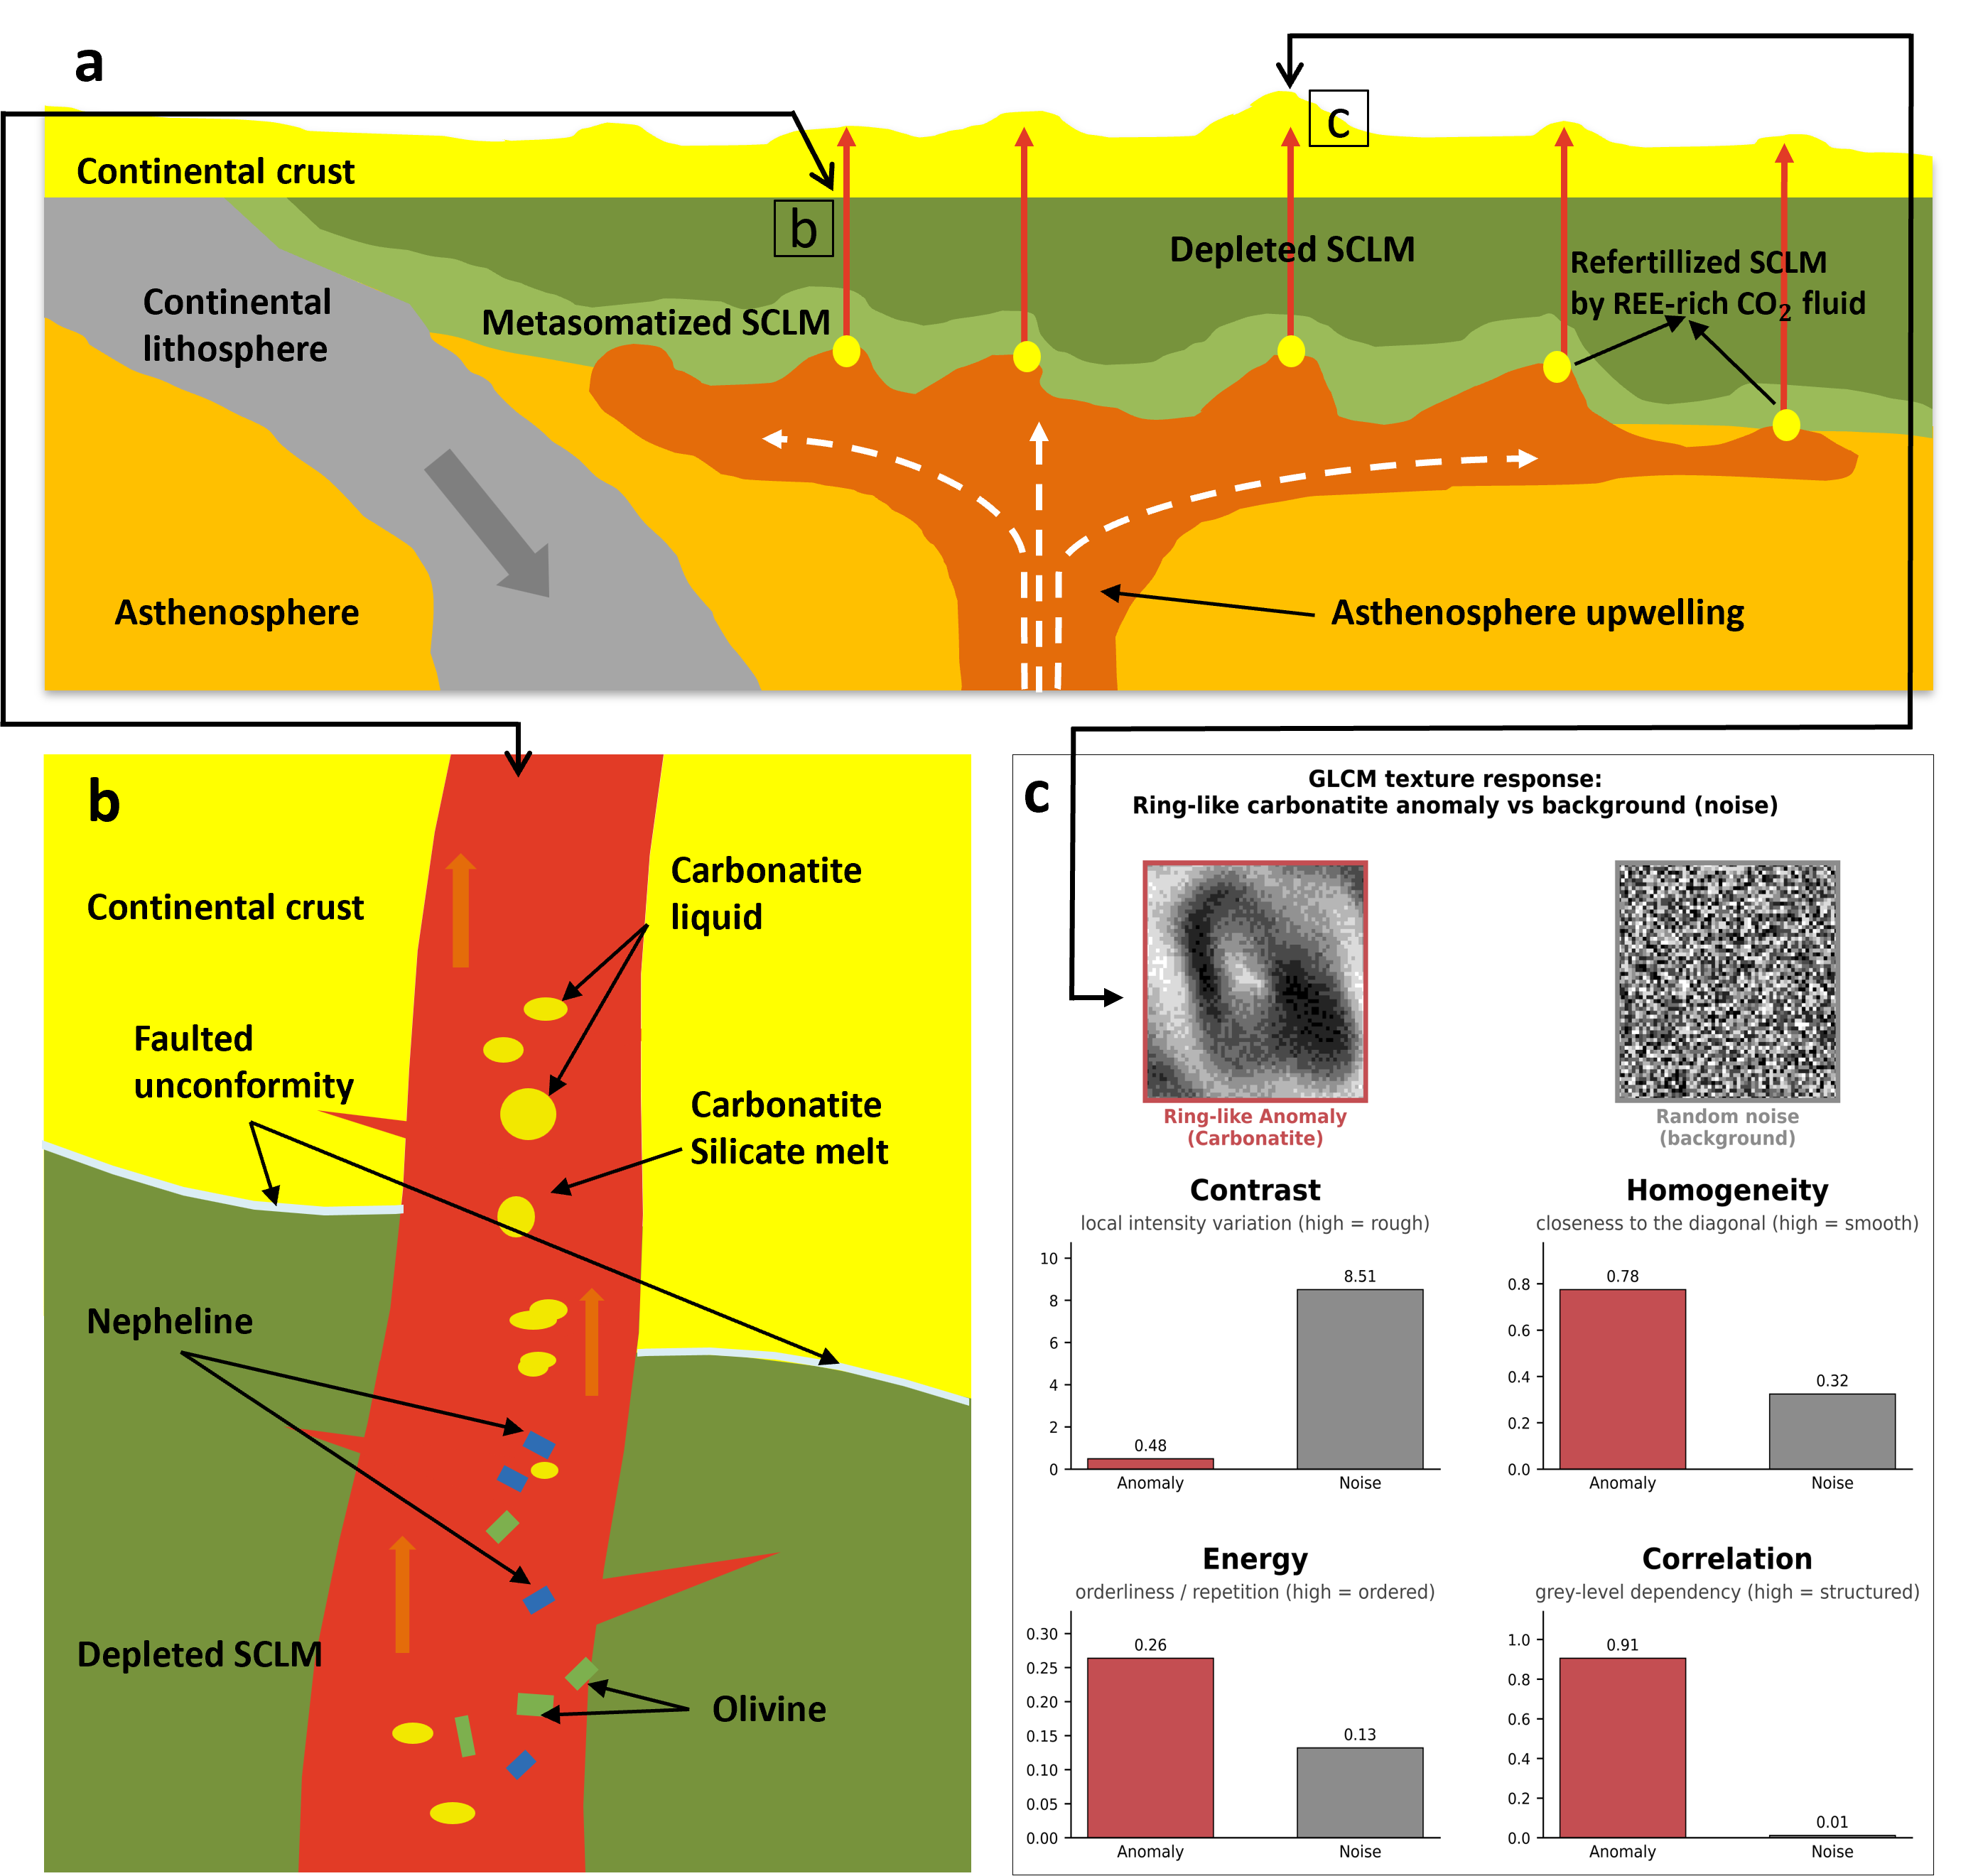
\includegraphics[width=0.85\textwidth]{figures/fig_mineral_system.png}
\caption{Source--transport--trap model for carbonatite-hosted REE systems and its geophysical proxies. (a) Source: refertilised subcontinental lithospheric mantle near the LAB at the craton margin, indexed by LAB depth and margin proximity; panel modified after \citet{Hou2023}. (b) Transport along trans-lithospheric faults, indexed by fault and worm proximity and Moho depth; modified after \citet{Yaxley2021}. (c) Trap: GLCM texture response of a ring-like anomaly and of random noise.}\label{fig:mineral-system}
\end{figure}

\subsection{Study areas}\label{sec:areas}

The three study areas are the Superior Province, the Grenville Province and the Cordilleran Orogen as outlined on the Geological Map of Canada \citep[Map 1860A;][]{Wheeler1996}. Each is modelled independently because carbonatite-hosted occurrences of the Phanerozoic, accreted Cordillera are geophysically distinct from those of the Canadian Shield \citep{Parsa2024}, so a single cross-terrane model would not be expected to transfer.

The Superior Province is the world's largest Archean craton. Carbonatite--alkaline magmatism in the Canadian Shield clusters into episodes at about 2.68~Ga, 1.90--1.88~Ga and 1.16--1.08~Ga \citep{Rukhlov2010}, and in the Superior Province many of the complexes are aligned along crustal-scale structures, most prominently the Kapuskasing Structural Zone \citep[KSZ;][]{Percival1994,Gittins1967}. The 15 Superior occurrences used here (Fig.~\ref{fig:study}b) comprise a cluster around the Montviel and Lac Shortt carbonatites in the eastern Abitibi region of Qu\'ebec (Deposit/Prospect and Showing class) and occurrences dispersed across the southern and western Superior Province, including Nemegosenda Lake, Lackner Lake, Kapuskasing, Martison Lake, Prairie Lake and Carb Lake. The Superior Province thus combines the fewest occurrences per unit area of the three provinces with a spatial structure, one tight cluster plus scattered singletons, in which a model can either learn the cluster or learn what the scattered occurrences have in common.

\begin{figure}[t]
\centering
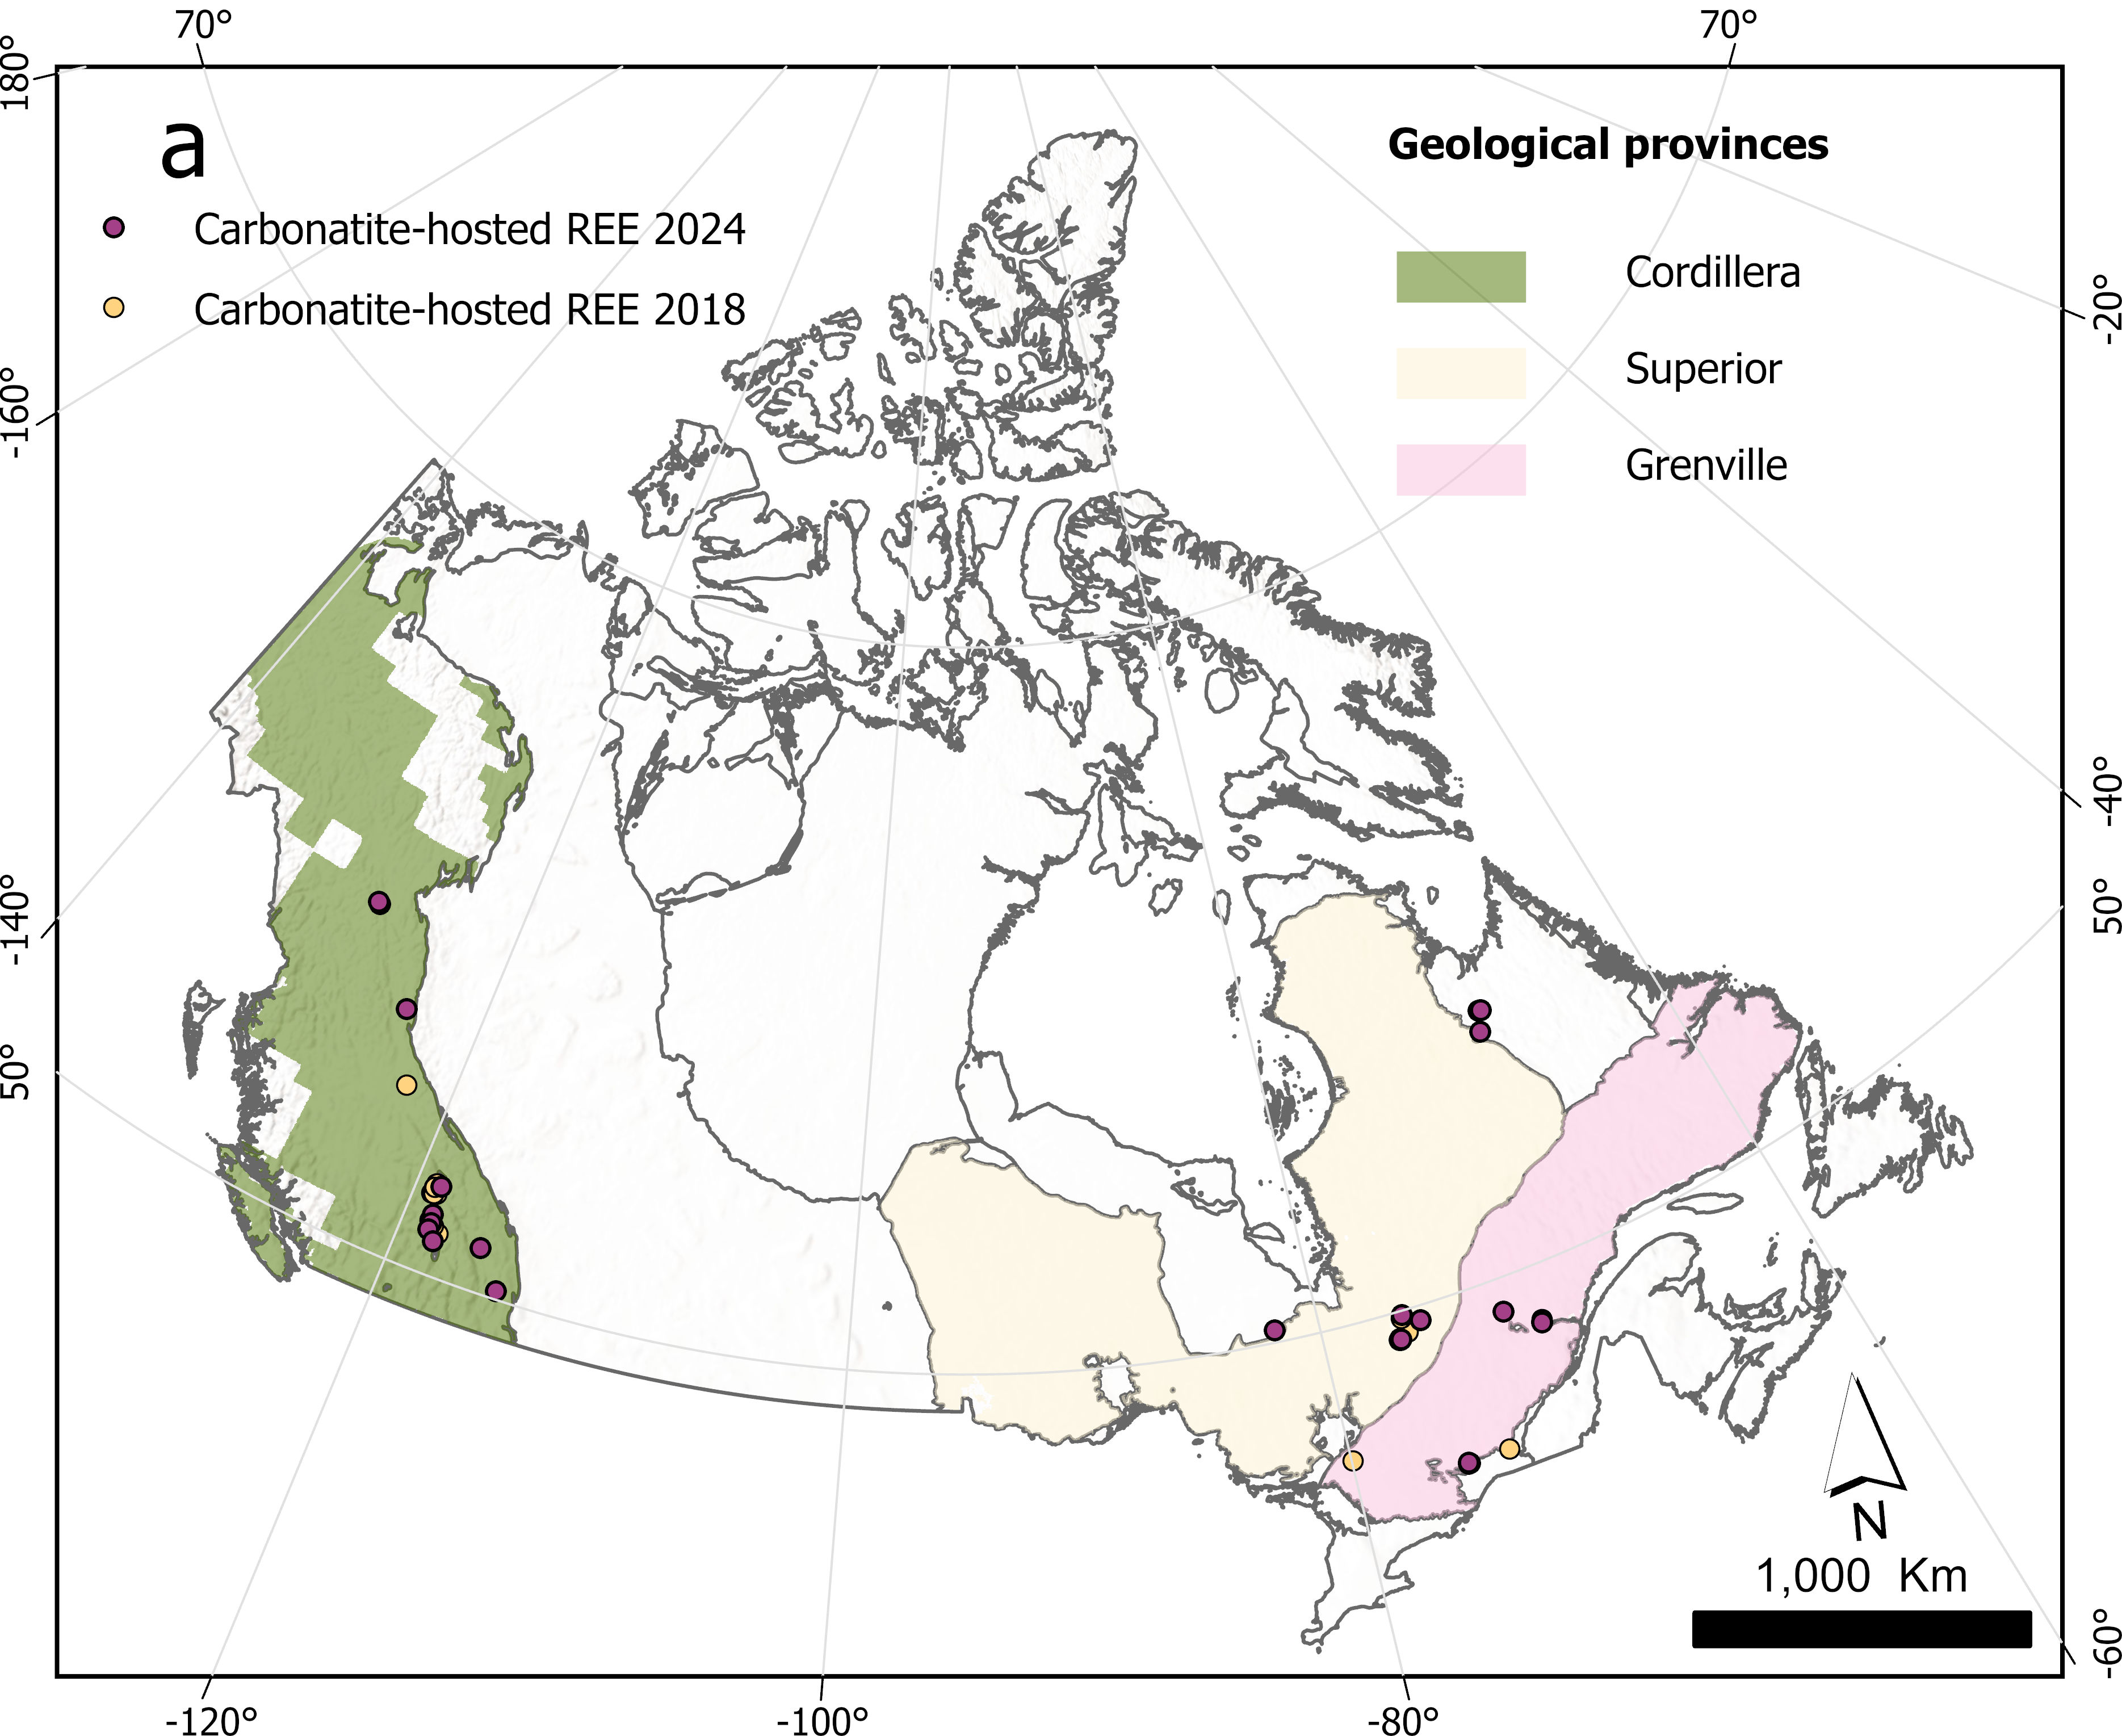
\includegraphics[width=0.55\textwidth]{figures/fig_study_canada.jpg}\hfill
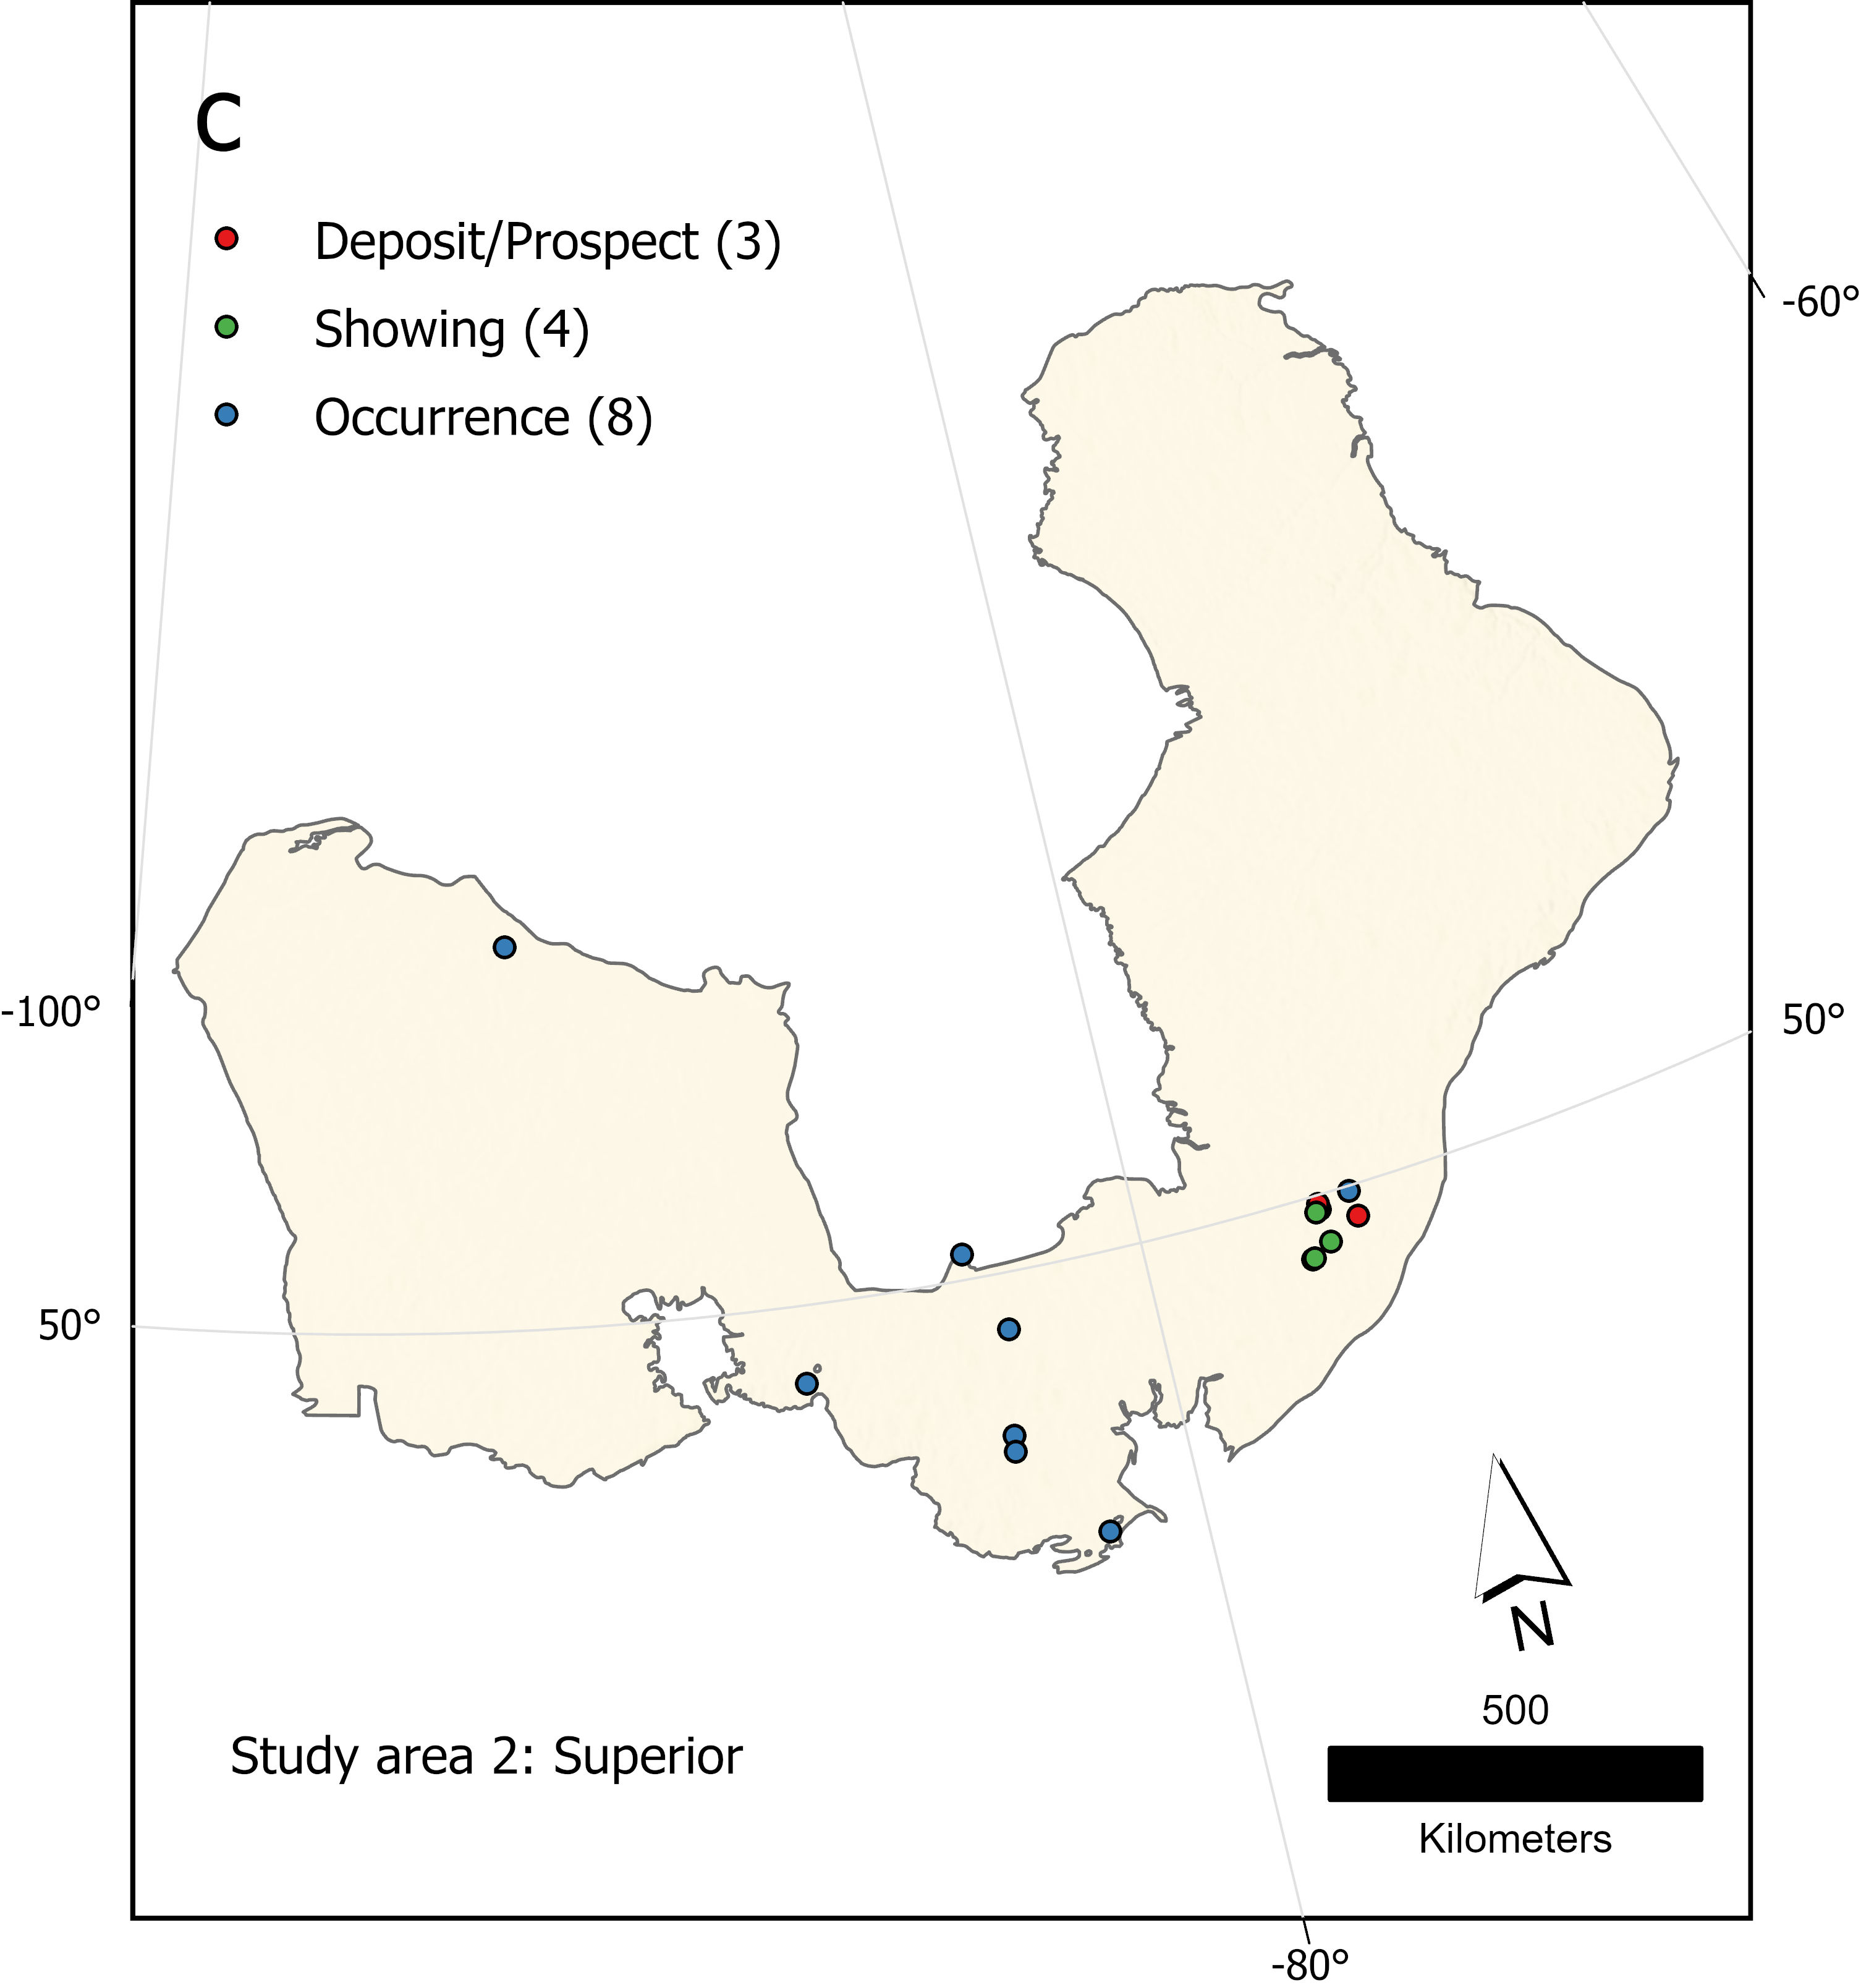
\includegraphics[width=0.42\textwidth]{figures/fig_study_superior.jpg}
\caption{(a) Carbonatite-hosted REE occurrences in Canada and the three modelled provinces; coloured areas are the sampleable domains. (b) The 15 deduplicated Superior occurrences used as positives, by development class.}\label{fig:study}
\end{figure}

\subsection{Occurrence labels}\label{sec:labels}

Positive labels were compiled from the carbonatite-hosted records of the USGS global REE occurrence database \citep{Orris2018} and the occurrence table of \citet{Parsa2024}. Alkaline-hosted occurrences were excluded after a preliminary leave-block-out classification showed them to be geophysically separable from carbonatite-hosted ones. Records within 2~km of each other were merged by single linkage, so that drill holes or zones of one deposit, listed once or in both sources, count once; without this step near-identical points from one deposit fall into both training and validation folds. Merging and the data-coverage filter (Section~\ref{sec:domain}) reduced 21, 13 and 51 pooled records to 15 (Superior), 12 (Grenville) and 27 (Cordillera) positives. Each positive keeps the development class of \citet{Parsa2024}: Deposit/Prospect, Showing or Occurrence (Superior: 3, 4 and 8).

\subsection{Geophysical and structural evidence layers}\label{sec:layers}

Table~\ref{tab:layers} lists the evidence layers. Seventeen national rasters cover the trap and the deep-architecture components: Bouguer gravity and its derivatives and filtered versions, total magnetic intensity and its differential reduction to the pole with derivatives \citep{Jobin2017,Miles2016}, together with long-wavelength gravity and magnetics, LAB and Moho depth from the Tri-National Critical Minerals Mapping Initiative release \citep{McCafferty2023}. Eleven of the gravity and magnetic grids are processed products supplied by Getech Group plc; four of these are gridded versions of the public Natural Resources Canada compilations and seven are standard derivatives of them (Table~\ref{tab:layers}). Two line layers (ancient passive margins, \citealp{BradleyDC2008}; faults) and four point layers (shallow and deep gravity and magnetic worms; \citealp{McCafferty2023}) enter as normalised proximities. GLCM contrast, homogeneity, energy and correlation were computed in 9$\times$9-pixel windows on the Bouguer anomaly, its 40~km high-pass, the reduced-to-pole magnetics and the total magnetic intensity. Following \citet{Luo2026}, the mean and standard deviation of the same four grids within 10~km of each point were added as neighbourhood statistics. Radiometric grids (K, eU, eTh) were considered but not used, because their coverage of the study areas is incomplete and uneven; whole-rock geochemistry is too sparse to give a value at every map cell. The province polygons of \citet{Wheeler1996} define the study areas only; no distance-to-province-boundary feature was used.

\begin{table}[t]
\caption{Evidence layers, grouped by mineral-system component. Native resolution in brackets. All rasters were sampled at points in their native projection and resolution.}\label{tab:layers}
\footnotesize
\begin{tabular*}{\textwidth}{@{\extracolsep\fill}p{2.3cm}p{6.0cm}p{3.2cm}}
\toprule
Component & Layer(s) & Source \\
\midrule
Source / lithosphere & Depth to LAB (0.1$^\circ$); Moho depth (0.25$^\circ$) & \citet{McCafferty2023} \\
Deep architecture & Bouguer gravity upward-continued 30~km and its horizontal-gradient magnitude (HGM) (0.031$^\circ$); long-wavelength (deep-source) RTP magnetics and its HGM (0.02$^\circ$) & \citet{McCafferty2023} \\
%% TODO(author): confirm the provenance of the fault compilation (KNOWN_ISSUES.md #3)
Transport & Proximity to faults; to ancient passive margins; to shallow and deep gravity and magnetic worms & \citet{McCafferty2023}; \citet{BradleyDC2008} \\
Trap: gravity & Bouguer anomaly (BA), BA first vertical derivative, BA total horizontal derivative (THD) (2~km) & \citet{Jobin2017}; gridded by Getech \\
 & BA THD tilt, BA 40~km and 100~km high-pass (4th-order Butterworth) (2~km) & Getech derivatives \\
Trap: magnetics & Total magnetic intensity (TMI) (0.01$^\circ$) & \citet{Miles2016}; gridded by Getech \\
 & Differential reduction to pole (DRTP), DRTP 1VD, DRTP THD, DRTP THD tilt (0.01$^\circ$) & Getech derivatives \\
Anomaly form & GLCM contrast, homogeneity, energy, correlation (9$\times$9 window) on BA, BA 40~km high-pass, DRTP, TMI; mean and standard deviation within 10~km of the same grids & this study \\
Geology & H3 cell (resolution 7): major lithology class, era, lithological- and age-contact flags; distances to contacts and units of a generalised map (Section~\ref{sec:featuresets}) & \citet{Wheeler1996} \\
\botrule
\end{tabular*}
\end{table}

\subsection{Geology}\label{sec:featuresets}

Geology enters from a hexagonal H3 grid (resolution 7, cells of about 5~km$^2$) attributed from the Geological Map of Canada \citep{Wheeler1996}. Each cell carries a major lithology class (for example Igneous Intrusive Alkalic or Metamorphic Gneiss Paragneiss), its dominant era, and flags for cells crossed by a lithological or an age (period) contact; each point takes the attributes of the cell that contains it. The lithology class enters as one-hot columns (a class gets its own column if at least 10 of the region's 5,000 training-background points fall in it; rarer classes share one), together with the era one-hot and the two contact flags. Following \citet{Luo2026}, geology also enters as distances (km) to six elements of a generalised map, from which every lithological unit smaller than 20 connected cells (about 100~km$^2$) and the alkalic-intrusion class were removed: lithological contacts, age contacts, greenstone (extrusive) units, mafic--ultramafic intrusions, high-grade metamorphic units and sedimentary units. After pruning (Section~\ref{sec:pruning}) the inputs number 48 in Superior (24 geophysical and structural layers, 3 neighbourhood statistics, 2 regional distances, 15 lithology columns, 2 era columns and 2 contact flags), 55 in Cordillera and 58 in Grenville.

At the scale of a carbonatite complex a bedrock map can mark the target itself: in Superior, 6 of the 15 occurrences fall on cells mapped as alkalic intrusive rock, against 16 of the 3,000 evaluation-background points (0.5\%). A mapped alkaline complex is legitimate evidence for an explorer, but a model can score well simply by looking it up. We therefore also report the models without the point-level map classes (the lithology, era and contact columns), keeping the geophysical and structural layers, neighbourhood statistics and regional distances (29, 31 and 33 inputs after pruning). This measures what the models achieve on ground where the map does not show a complex.

\subsection{Sampleable domain and background}\label{sec:domain}

Rasters were clipped to each study-area outline buffered outward by one GLCM window radius (8~km), so that windows near the boundary read real data, and sampling and prediction were restricted to the domain where every layer holds data and every texture window is computable. This domain covers 98.6\% of the Superior, 97.2\% of the Grenville and 73.5\% of the Cordilleran outline; one Cordilleran occurrence (Lempriere) falls outside it and was dropped. Background candidates are the nodes of a 0.1$^\circ$ grid inside the domain and more than 10~km from any known occurrence (19,371 in Superior). From these, two disjoint pools were drawn once per region at random: an evaluation background of 3,000 points and a training background of 5,000 points. Every model in this study is trained on the positives of its training fold plus the same 5,000 training-background points and scored on the held-out positives plus the same evaluation background. The prevalence in the scored pool is therefore 15/3,015 $\approx$ 0.5\% in Superior, which is the AP of a random ranking.

%% ===================================================================
\section{Methods}\label{sec:methods}

Figure~\ref{fig:workflow} summarises the workflow. Code for every analysis, including the exact numbers in every table, is available in the repository listed under Code availability.

\begin{figure}[t]
\centering
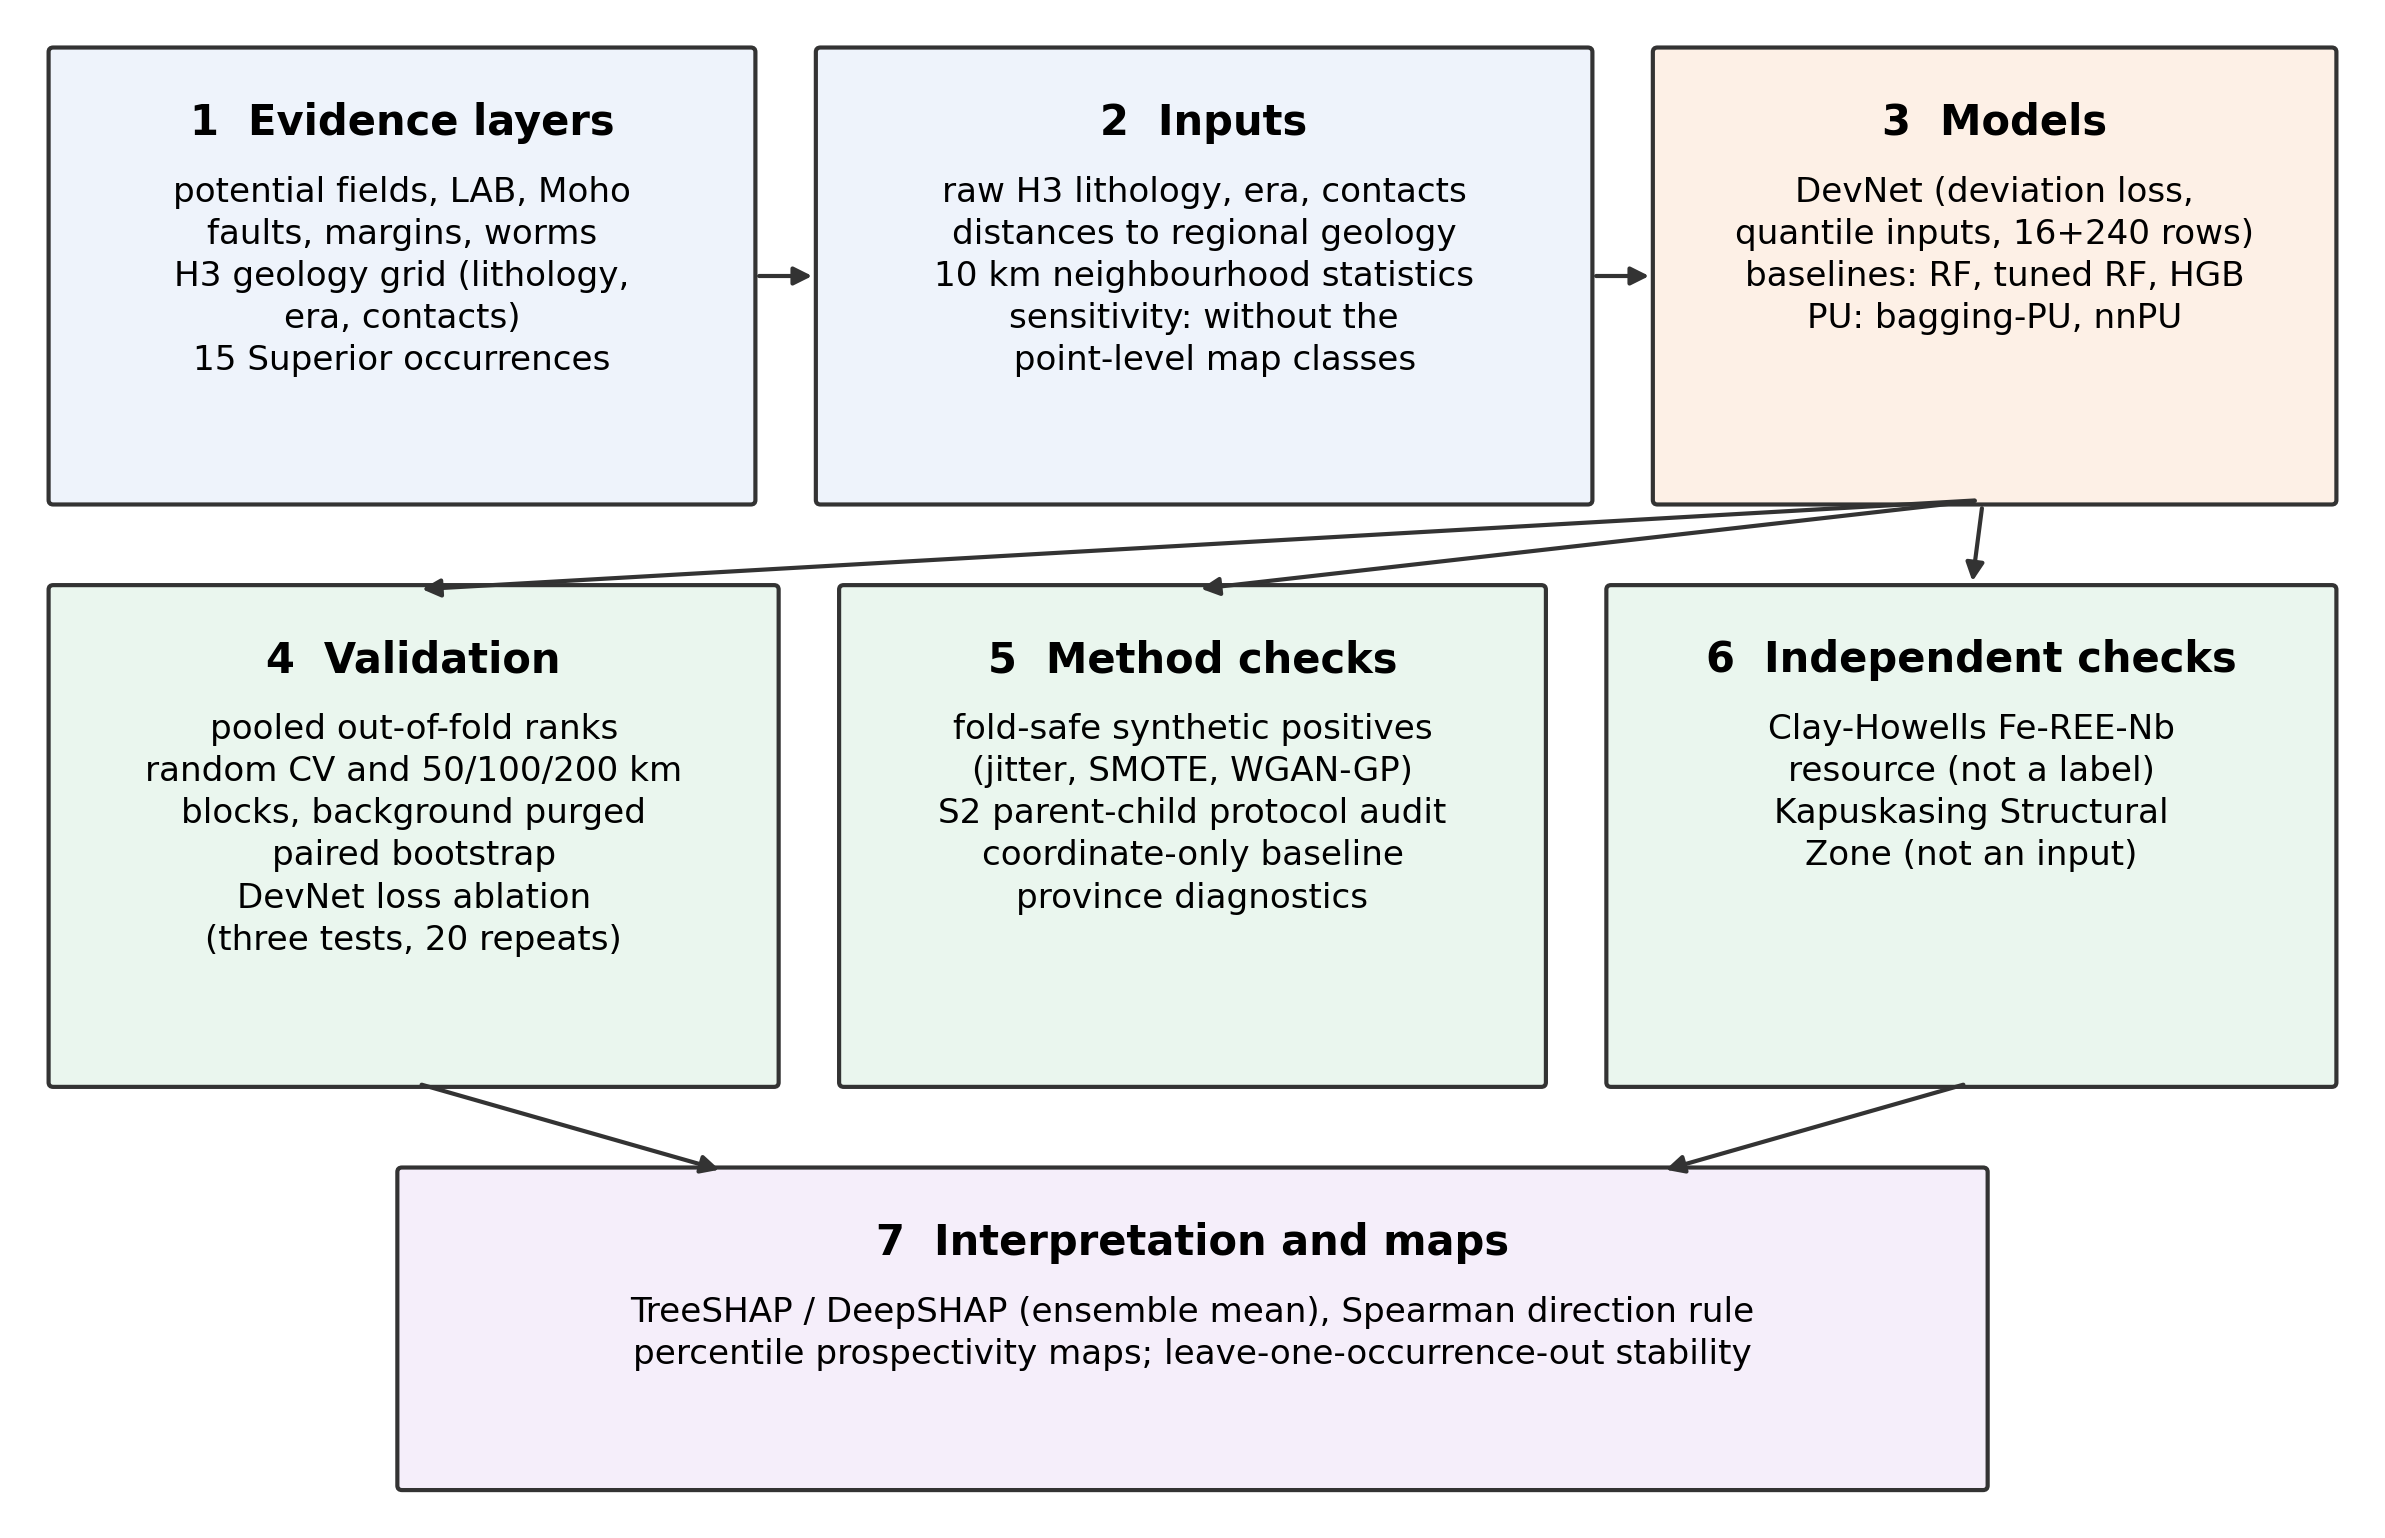
\includegraphics[width=\textwidth]{figures/fig_workflow_r4.png}
\caption{Workflow. All models are trained on the same positives and the same 5,000 background points and scored on the same folds; only the treatment of the background, or the loss, differs.}\label{fig:workflow}
\end{figure}

\subsection{Feature pruning}\label{sec:pruning}

The candidate features include many collinear geophysical derivatives. Within each region, features were clustered hierarchically on $1-|\rho_{\mathrm{S}}|$ (Spearman correlation, average linkage) and cut at $|\rho_{\mathrm{S}}| = 0.7$, keeping one representative per cluster chosen by lowest missing rate and then highest variance \citep{Dormann2013}. The rule never sees labels and therefore cannot leak information across folds.

\subsection{Models}\label{sec:models}

All models see the same rows and differ only in how they treat the training background or in their loss.

\textbf{Random Forest} (RF; \citealp{Breiman2001}) is the discriminative baseline: positives versus training background labelled 0, 300 trees, $\sqrt{p}$ features per split, balanced class weights, inside a pipeline that fits median imputation and standardisation on the training fold only. With roughly 12 training positives against 5,000 background points, most held-out points receive a predicted probability of exactly zero, so the pooled AUC depends on which trees happen to vote for a given held-out occurrence. We therefore vary the RF seed across folds so that this variance enters the reported intervals.

\textbf{DevNet} \citep{Pang2019} maps each input vector $\mathbf{x}$ to a scalar score $\phi(\mathbf{x})$ through one hidden ReLU layer with dropout. The deviation $d(\mathbf{x}) = (\phi(\mathbf{x}) - \mu_R)/\sigma_R$ is measured against the mean and standard deviation of a fixed reference sample of 50,000 standard-normal draws, and the loss
\begin{equation}
L = (1-y)\,|d(\mathbf{x})| + y\,\max\{0,\, a - d(\mathbf{x})\}
\end{equation}
pulls unlabelled background ($y=0$) towards the reference and pushes positives ($y=1$) beyond a margin $a = 5$, the value of \citet{Pang2019} (Appendix~\ref{app:sensitivity}, Table~\ref{tab:margin}). Network capacity was set a priori by positive count (64 hidden units, dropout 0.3, weight decay $10^{-4}$ in Cordillera; 32, 0.4 and $10^{-3}$ in Superior and Grenville) rather than tuned, because a search over a few tens of positives fits noise. Training uses Adam \citep{Kingma2014} with weight decay, cosine learning-rate annealing over 300 steps and gradient clipping, and each fold score is the rank average of five restarts with different seeds.

Two design choices adapt DevNet to tabular evidence layers with very few positives. First, inputs are mapped to standard-normal marginals by a quantile transformation fitted on each training fold. Many evidence layers are strongly skewed (inverted distances concentrated near 0 or 1, long-tailed textures, 0/1 dummies), and unlike tree ensembles, which are invariant to monotone transformations, multilayer perceptrons are sensitive to such marginal distributions \citep{Gorishniy2021,Grinsztajn2022}. Second, each gradient step uses 16 positives (resampled with replacement) and 240 background rows. The deviation loss is meant to learn what the background looks like; with label-balanced batches of 16 + 16 rows, 300 steps would show each background row about once and each positive about 400 times, whereas background-heavy batches show each background row about 14 times while positive exposure is unchanged. Both choices were settled with diagnostic runs on these provinces using an earlier, coarser encoding of the geology; Appendix~\ref{app:sensitivity} repeats the ablation with the inputs used here.

\textbf{Bagging-PU} \citep{Mordelet2014} trains 200 fully grown decision trees, each on all training positives and an equal-sized bootstrap sample of the unlabelled background, and averages their outputs. It is the standard tree-based PU learner and the closest PU analogue of RF.

\textbf{nnPU} \citep{Kiryo2017} minimises the non-negative PU risk with the sigmoid loss, using exactly DevNet's network, quantile-normal inputs, optimiser, number of steps and five-restart ensemble, so that DevNet versus nnPU isolates the PU risk from the deviation loss. nnPU requires the class prior $\pi = P(y=1)$ in the unlabelled population; we use $\pi = 0.01$ (sensitivity in Appendix~\ref{app:full}, Table~\ref{tab:prior}). The calibration approach of \citet{Elkan2008} is not included because under its assumptions the calibrated output is a monotone transform of the positive-versus-background classifier, so its ranking, and every rank metric reported here, equals RF's.

\textbf{RF-tuned and HGB-tuned} give the tree-based baselines a design search of their own. Inside every outer training fold, an inner spatially blocked cross-validation (100~km blocks, three folds, training background purged from inner validation blocks) chooses the RF's minimum leaf size (1 or 10) and number of features per split ($\sqrt{p}$ or $p/3$), or the number of leaves (8 or 31) and minimum leaf size (5 or 40) of a histogram gradient-boosting classifier \citep{Pedregosa2011} with balanced class weights, 200 iterations, learning rate 0.05 and an L2 penalty of 1. The outer test fold is never used for the choice.

\subsection{Evaluation protocol}\label{sec:protocol}

With three or four positives per validation fold, per-fold AUC is unstable and can be undefined, so out-of-fold scores are pooled \citep{BradleyAP1997}: each held-out point is scored once per repeat, scores are converted to within-fold percentile ranks so that folds are comparable, and a single AUC and average precision (AP) are computed over all folds. Pooling carries a small known negative bias in AUC \citep{Airola2019,Parker2007}. We emphasise AP because, at 0.5\% prevalence, it reflects the practical task of concentrating occurrences into a small search area, whereas AUC is dominated by the bulk of easily rejected background \citep{Saito2015}. Exploration efficiency is also shown as capture-rate curves: the share of held-out occurrences ranked within a given top fraction of the scored pool \citep{Chung2003,Agterberg2005}. Because the evaluation background is a random sample of the domain, this fraction approximates search area. Because unexplored background may host undiscovered occurrences, all metrics are conservative.

\textbf{Random cross-validation.} Repeated stratified 5-fold cross-validation with six repeats gives six pooled AUC and AP values per model, reported as the median and the 2.5--97.5 percentile interval over repeats (labelled 95\% interval). All models use identical splits, so they can be compared pairwise.

\textbf{Spatially blocked cross-validation.} Random folds can hold out an occurrence a few kilometres from a training occurrence. Following \citet{Roberts2017} and \citet{Valavi2019}, labelled points were assigned to square blocks of 50, 100 or 200~km side in Canada Atlas Lambert (EPSG:3978), whole blocks were held out together using stratified group 5-fold splitting (fewer folds if fewer blocks contain positives), and every training-background point falling inside a held-out block was removed from training for that fold. Each of six repeats uses a random offset of the block grid.

\textbf{Paired comparisons.} For each pair of models we average each point's out-of-fold rank over the six repeats and draw 5,000 stratified bootstrap resamples of positives and background \citep{Efron1993}, reporting the difference in AP and AUC with its 95\% percentile interval and the number of the six repeats in which the first model has the higher AP. With 12--27 positives these comparisons have little power, so we treat a difference as established only when it is consistent across repeats, block sizes and provinces.

\textbf{Geography-only baseline.} To separate geological signal from spatial memorisation, an RF was trained on the projected coordinates of each point only, with no evidence layer, under the same folds and both protocols. Its score measures how much of a protocol's reported skill can be obtained simply by remembering where the training occurrences lie. An L2-regularised logistic regression with balanced class weights serves as a smooth, essentially linear discriminative reference.

\subsection{Ablation of the deviation loss}\label{sec:ablation-methods}

DevNet differs from the other learners in three respects: its deviation loss, which treats the training background as unlabelled ground to be described rather than as barren ground to be separated from the occurrences; its rank-normal inputs; and its background-heavy batches. To isolate the first, \textbf{DevNet-BCE} keeps DevNet's network, inputs, batches, training length and five-restart ensemble but replaces the deviation loss by binary cross-entropy with the background labelled 0. DevNet-BCE is not a competing prospectivity method but DevNet with one component changed. The tree-based pair, RF (background labelled 0) and bagging-PU (background unlabelled), gives the same contrast for tree ensembles.

The premise of treating the background as unlabelled is that it contains undiscovered occurrences and ground that resembles them. If the premise matters, a loss that treats the background as barren should suffer more when the background holds such ground, and a semi-supervised loss should profit more from a large unlabelled pool and when labels are scarcest. We tested these three predictions, written down before the runs, with 20 repeats instead of six, with and without the point-level map classes, under random cross-validation and 100~km blocks, first in Superior and then, unchanged, in Cordillera and Grenville.
\textit{(E1) Mislabelled ground near occurrences.} The main design excludes background within 10~km of every occurrence. Here 0, 20 or 50 additional background points per occurrence, drawn uniformly in a 2--10~km annulus around each occurrence, were added to the training background; under random cross-validation this includes ground around the held-out occurrences, as in practice the unlabelled pool contains ground around undiscovered deposits. Prediction: DevNet-BCE loses more AP than DevNet, and RF more than bagging-PU.
\textit{(E2) Size of the unlabelled pool.} The training background was a nested random subset of 625, 1,250, 2,500 or 5,000 points. Prediction: DevNet's lead over DevNet-BCE grows with the pool.
\textit{(E3) Label scarcity.} All but $k = 1, 2, 3, 5$ or 8 training positives per fold were dropped, the same ones for every model. Prediction: DevNet is ahead of DevNet-BCE for $k \leq 3$, more so without map classes.
For each pair of models and each repeat (identical folds for both models and all conditions) we computed the predicted effect (E1: the difference between the two models' AP changes from 0 to 50 added points; E2: the change in their AP gap from 625 to 5,000 points; E3: their AP difference averaged over $k = 1$--3) and report its median and the number of the 20 repeats in which it favours the unlabelled-background model.

\subsection{Other analyses}\label{sec:robust-methods}

\textbf{Nested design selection.} DevNet's input transformation and batch composition were settled with diagnostic runs on these three provinces, so its scores may carry selection optimism. To measure it, the choice among the four combinations of z-scored or quantile-normal inputs and 16 or 240 background rows per step was made inside every outer training fold by the inner spatial cross-validation described above (two restarts per candidate), and the chosen design, refitted on the whole outer training fold, scored the outer test fold.

\textbf{Map stability.} Each Superior occurrence was left out in turn and the production models were refitted on the other 14; for every grid node we report the share of these 15 models that place it in the province's top 5\%. Prediction--area curves \citep{YousefiCarranza2015} were computed from the out-of-fold ranks, with the evaluation background as a proxy for area.

\textbf{Province diagnostics.} To describe, independently of any model, why skill differs between provinces, each label set was characterised by its number of independent sites (occurrences merged by single linkage at 10~km), the share of occurrences that share a site with another and the median distance to the nearest other occurrence. The signal shared by distant occurrences was measured with a far-neighbour index: with features expressed as percentile ranks, it is, for each occurrence, the share of background points more than 100~km away that are closer to it in feature space than the most similar occurrence more than 100~km away. A value near 0 means that distant occurrences resemble one another more than they resemble almost any background. The median over occurrences, computed on the geophysical and structural layers, is compared with the same statistic for 200 sets of background points drawn at random to pose as occurrences.

\subsection{Synthetic positives}\label{sec:augmentation}

To test whether synthetic positives can compensate for label scarcity, each training fold's real positives were augmented with $m \times n_{\mathrm{pos}}$ synthetic positives ($m = 1, 3, 10$) before RF and DevNet were retrained; the held-out positives were always real. Three generators were compared, all fitted in the standardised feature space of the training fold only: Gaussian jitter of real positives ($\sigma = 0.1$ standard deviations); SMOTE-style interpolation between a positive and one of its three nearest positive neighbours \citep{Chawla2002}; and a tabular Wasserstein GAN with gradient penalty \citep[WGAN-GP;][]{Goodfellow2014,Arjovsky2017,Gulrajani2017} with an eight-dimensional latent input, two hidden layers of 64 units in generator and critic, five critic updates per generator update, gradient-penalty weight 10 and 2,000 generator updates, trained on the fold's 12 positives. Synthetic geology columns were snapped back to valid one-hot and 0/1 values. To see what the generators produce, each was also fitted to all 15 Superior positives and 150 samples were characterised by the distance to the nearest real positive divided by the median nearest-neighbour distance among real positives (a value near 0 indicates copying), by the share of samples whose nearest labelled neighbour is a positive rather than a background point, and by their DevNet score percentile.

\subsection{Validation-protocol audit}\label{sec:audit-methods}

To quantify how the validation design of \citet{Parsa2024} behaves on these data, we rebuilt it with the same S2 geometry library. Each occurrence's level-12 S2 cell (about 4.5~km$^2$) was replaced by its four level-13 child cells, and all inputs were extracted at the child-cell centres with the same pipeline. An equal number of negatives was drawn either from the 5\% of background candidates with the lowest mean cosine similarity to the augmented positives in min--max scaled feature space (as described by \citealp{Parsa2024}) or at random. Random forests of 1,000 trees on min--max scaled features were evaluated with 50 stratified 70/30 splits. Three split designs were compared: (i) child-level random splitting, as described in the original study; (ii) splitting with all children of one parent kept on the same side; and (iii) no augmentation, one label per occurrence. We report mean test AUC, its 2.5--97.5 percentile range over the 50 splits, and the share of test positives with a sibling in the training set. The audit uses our inputs, regions and models rather than those of the original study, so it measures the sensitivity of the protocol, not the original study's numbers.

\subsection{Interpretation and mapping}\label{sec:shap}

Production models were fitted to all positives and the training background of each region. SHAP values \citep{Lundberg2017} were computed with TreeSHAP for RF \citep{Lundberg2020} and DeepSHAP for DevNet on an explain set of all positives plus evaluation-background points (200 in total), with 100 training-background points as DevNet's reference sample; DevNet's SHAP values refer to its quantile-transformed inputs, which leaves the rank-based directions defined below unaffected. DevNet SHAP values were averaged over the five ensemble members. Importance is mean $|$SHAP$|$. The \emph{direction} of a feature's effect is the Spearman correlation between the feature's value and its SHAP value over the explain set (for one-hot dummies, the sign of the mean SHAP difference between presence and absence), with $|\rho| < 0.1$ reported as no clear direction. We do not use the sign of the mean SHAP value, which reflects where the explained points lie relative to the explainer's baseline rather than whether higher feature values raise the score: for RF with balanced class weights the TreeSHAP baseline is near 0.5 while nearly all explained points score near 0, so that rule would label every RF feature as ``higher $\rightarrow$ less prospective''. Prospectivity maps classify each model's scores on a 0.1$^\circ$ prediction grid into the top 1\%, 5\% and 10\%, because DevNet's anomaly score and RF's probability are not on a common scale. As an external check, the production models scored Clay-Howells, a drill-tested Fe--REE--Nb prospect with reported resources on the KSZ \citep{OGS2011} that is not among the training labels, at its recorded location.

%% ===================================================================
\section{Results}\label{sec:results}

\subsection{Model comparison under random cross-validation}\label{sec:res-random}

In Superior all models except nnPU rank held-out occurrences far above chance (Table~\ref{tab:benchmark}): AP is 0.22--0.45 against a random-ranking value of 0.005, and AUC is 0.97--0.98. DevNet has the highest median AP (0.445) and RF the highest AUC (0.983). DevNet's AP exceeds RF's, bagging-PU's and nnPU's in all six repeated splits, by 0.21--0.26 on repeat-averaged ranks (Table~\ref{tab:bootstrap}). nnPU, which shares DevNet's network and inputs, reaches an AP of only 0.152 and an AUC of 0.838.

The contrasting regions behave differently. In Cordillera, bagging-PU and RF lead (AP 0.433 and 0.427) and DevNet trails (0.341; lower than RF in all six repeats). In Grenville all models are weak and RF leads (0.257), ahead of DevNet (0.125) in all six repeats. nnPU fails in both provinces (AUC 0.54--0.55). That Superior is the best-predicted of the three provinces agrees with the province-level success rates of \citet{Parsa2024}.

\begin{table}[t]
\caption{Pooled out-of-fold AUC and AP (median and 95\% interval over six repeated 5-fold random splits). Bold: best of the four models in each region.}\label{tab:benchmark}
\footnotesize
\begin{tabular*}{\textwidth}{@{\extracolsep\fill}llcc}
\toprule
Region ($n_{\mathrm{pos}}$) & Model & AUC & AP \\
\midrule
\multirow{4}{*}{Superior (15)} & DevNet & 0.972 & \textbf{0.445} [0.404, 0.474] \\
 & RF & \textbf{0.983} & 0.271 [0.165, 0.289] \\
 & Bagging-PU & 0.976 & 0.219 [0.158, 0.264] \\
 & nnPU & 0.838 & 0.152 [0.125, 0.191] \\
\midrule
\multirow{4}{*}{Cordillera (27)} & DevNet & 0.914 & 0.341 [0.299, 0.394] \\
 & RF & 0.931 & 0.427 [0.368, 0.516] \\
 & Bagging-PU & \textbf{0.936} & \textbf{0.433} [0.304, 0.507] \\
 & nnPU & 0.553 & 0.022 [0.019, 0.029] \\
\midrule
\multirow{4}{*}{Grenville (12)} & DevNet & 0.799 & 0.125 [0.054, 0.171] \\
 & RF & 0.838 & \textbf{0.257} [0.182, 0.489] \\
 & Bagging-PU & \textbf{0.898} & 0.191 [0.172, 0.255] \\
 & nnPU & 0.542 & 0.008 [0.006, 0.009] \\
\botrule
\end{tabular*}
\end{table}

\begin{table}[t]
\caption{Paired comparisons of DevNet with each other model (random cross-validation): difference in AP and AUC computed on repeat-averaged out-of-fold ranks, with 95\% stratified bootstrap interval, and the number of the six repeats in which DevNet has the higher AP.}\label{tab:bootstrap}
\footnotesize
\setlength{\tabcolsep}{3pt}
\begin{tabular*}{\textwidth}{@{\extracolsep\fill}llccc}
\toprule
Region & Comparison & $\Delta$AP [95\%] & AP wins & $\Delta$AUC [95\%] \\
\midrule
Superior & DevNet $-$ RF & +0.210 [+0.001, +0.424] & 6/6 & -0.012 [-0.032, +0.004] \\
Superior & DevNet $-$ Bagging-PU & +0.256 [+0.026, +0.471] & 6/6 & -0.006 [-0.028, +0.012] \\
Superior & DevNet $-$ nnPU & +0.244 [+0.053, +0.448] & 6/6 & +0.111 [+0.037, +0.189] \\
\addlinespace
Cordillera & DevNet $-$ RF & -0.093 [-0.228, +0.092] & 0/6 & -0.032 [-0.098, +0.012] \\
Cordillera & DevNet $-$ Bagging-PU & -0.084 [-0.222, +0.103] & 1/6 & -0.021 [-0.080, +0.023] \\
Cordillera & DevNet $-$ nnPU & +0.353 [+0.189, +0.570] & 6/6 & +0.359 [+0.199, +0.517] \\
\addlinespace
Grenville & DevNet $-$ RF & -0.258 [-0.446, -0.076] & 0/6 & -0.050 [-0.147, +0.077] \\
Grenville & DevNet $-$ Bagging-PU & -0.162 [-0.305, -0.018] & 0/6 & -0.108 [-0.180, -0.044] \\
Grenville & DevNet $-$ nnPU & +0.194 [+0.025, +0.453] & 6/6 & +0.262 [+0.044, +0.467] \\
\botrule
\end{tabular*}
\end{table}

\subsection{Spatially blocked validation}\label{sec:res-spatial}

Holding out whole blocks widens the gap between DevNet and the tree-based and PU learners in Superior (Fig.~\ref{fig:spatial}; Table~\ref{tab:spatial}). DevNet's AP is 0.418, 0.343 and 0.252 with 50, 100 and 200~km blocks. RF's falls from 0.271 under random splits to 0.192, 0.168 and 0.151, and bagging-PU's to 0.148, 0.129 and 0.090. DevNet has the higher AP than RF, bagging-PU and nnPU in all six repeats at every block size (Table~\ref{tab:spatial-boot}), by $+0.18$ to $+0.24$ against RF, $+0.25$ to $+0.33$ against bagging-PU and $+0.19$ to $+0.41$ against nnPU. With 15 occurrences, however, the 95\% intervals of the differences from RF reach down to about zero, so the margin over RF is consistent but not statistically conclusive; the margins over bagging-PU and nnPU are clearer. AUC tells a partly different story with 200~km blocks, where RF (0.880) and bagging-PU (0.855) exceed DevNet (0.783; Appendix~\ref{app:full}, Table~\ref{tab:spatial-auc}): DevNet ranks most held-out occurrences very high but misses a few almost entirely, notably Kapuskasing and Nemegosenda Lake.

Capture-rate curves (Fig.~\ref{fig:capture}) show where the AP differences arise. Under random splits DevNet and RF capture about half of the held-out occurrences in the top 1\% of the ranked pool (53\% and 50\%), and RF and bagging-PU capture all of them by the top 10\% (DevNet 93\%). With 50 and 100~km blocks DevNet keeps its top-1\% capture (53\% and 47\%) and captures 90--93\% by the top 10\%, whereas RF captures 43\% in the top 1\% and 83--90\% by the top 10\%, and bagging-PU 30\% and 83--90\%. With 200~km blocks every model captures 47\% or less in the top 1\%, and by the top 10\% RF and bagging-PU (70\%) slightly exceed DevNet (63\%). Prediction--area curves (Appendix~\ref{app:full}, Fig.~\ref{fig:pa}), which summarise the whole ranking rather than its top, do not separate the models.

In Cordillera every model degrades sharply under blocking (AP $\leq 0.17$ at 50~km and $\leq 0.09$ at 100--200~km), and in Grenville AP approaches the random-ranking value ($\leq 0.009$ at 100--200~km). In these regions no difference between models is of practical size: their random-split skill owes much to spatial proximity between training and test occurrences (Section~\ref{sec:res-geography}).

\begin{figure}[t]
\centering
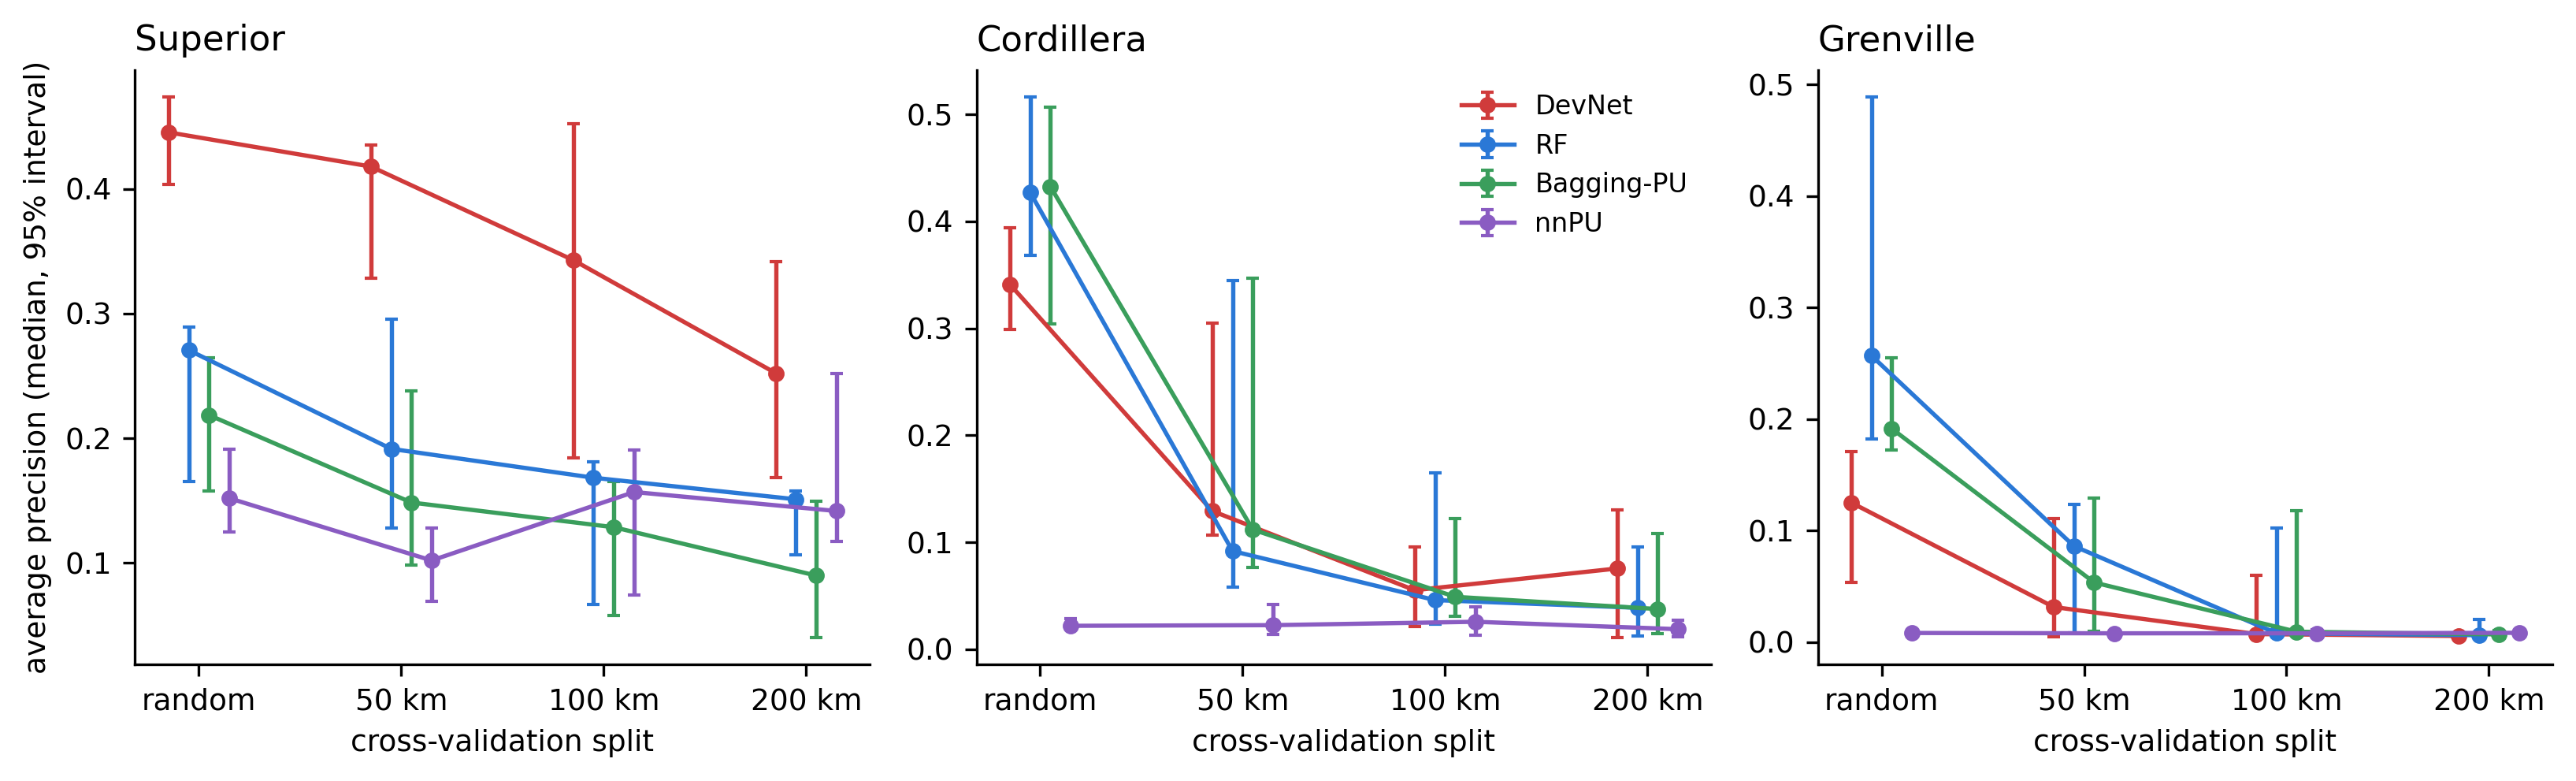
\includegraphics[width=\textwidth]{figures/fig_spatial_cv_r3.png}
\caption{Average precision under random and spatially blocked cross-validation (median and 95\% interval over six repeats). The random-ranking AP is 0.005 (Superior), 0.009 (Cordillera) and 0.004 (Grenville).}\label{fig:spatial}
\end{figure}

\begin{figure}[t]
\centering
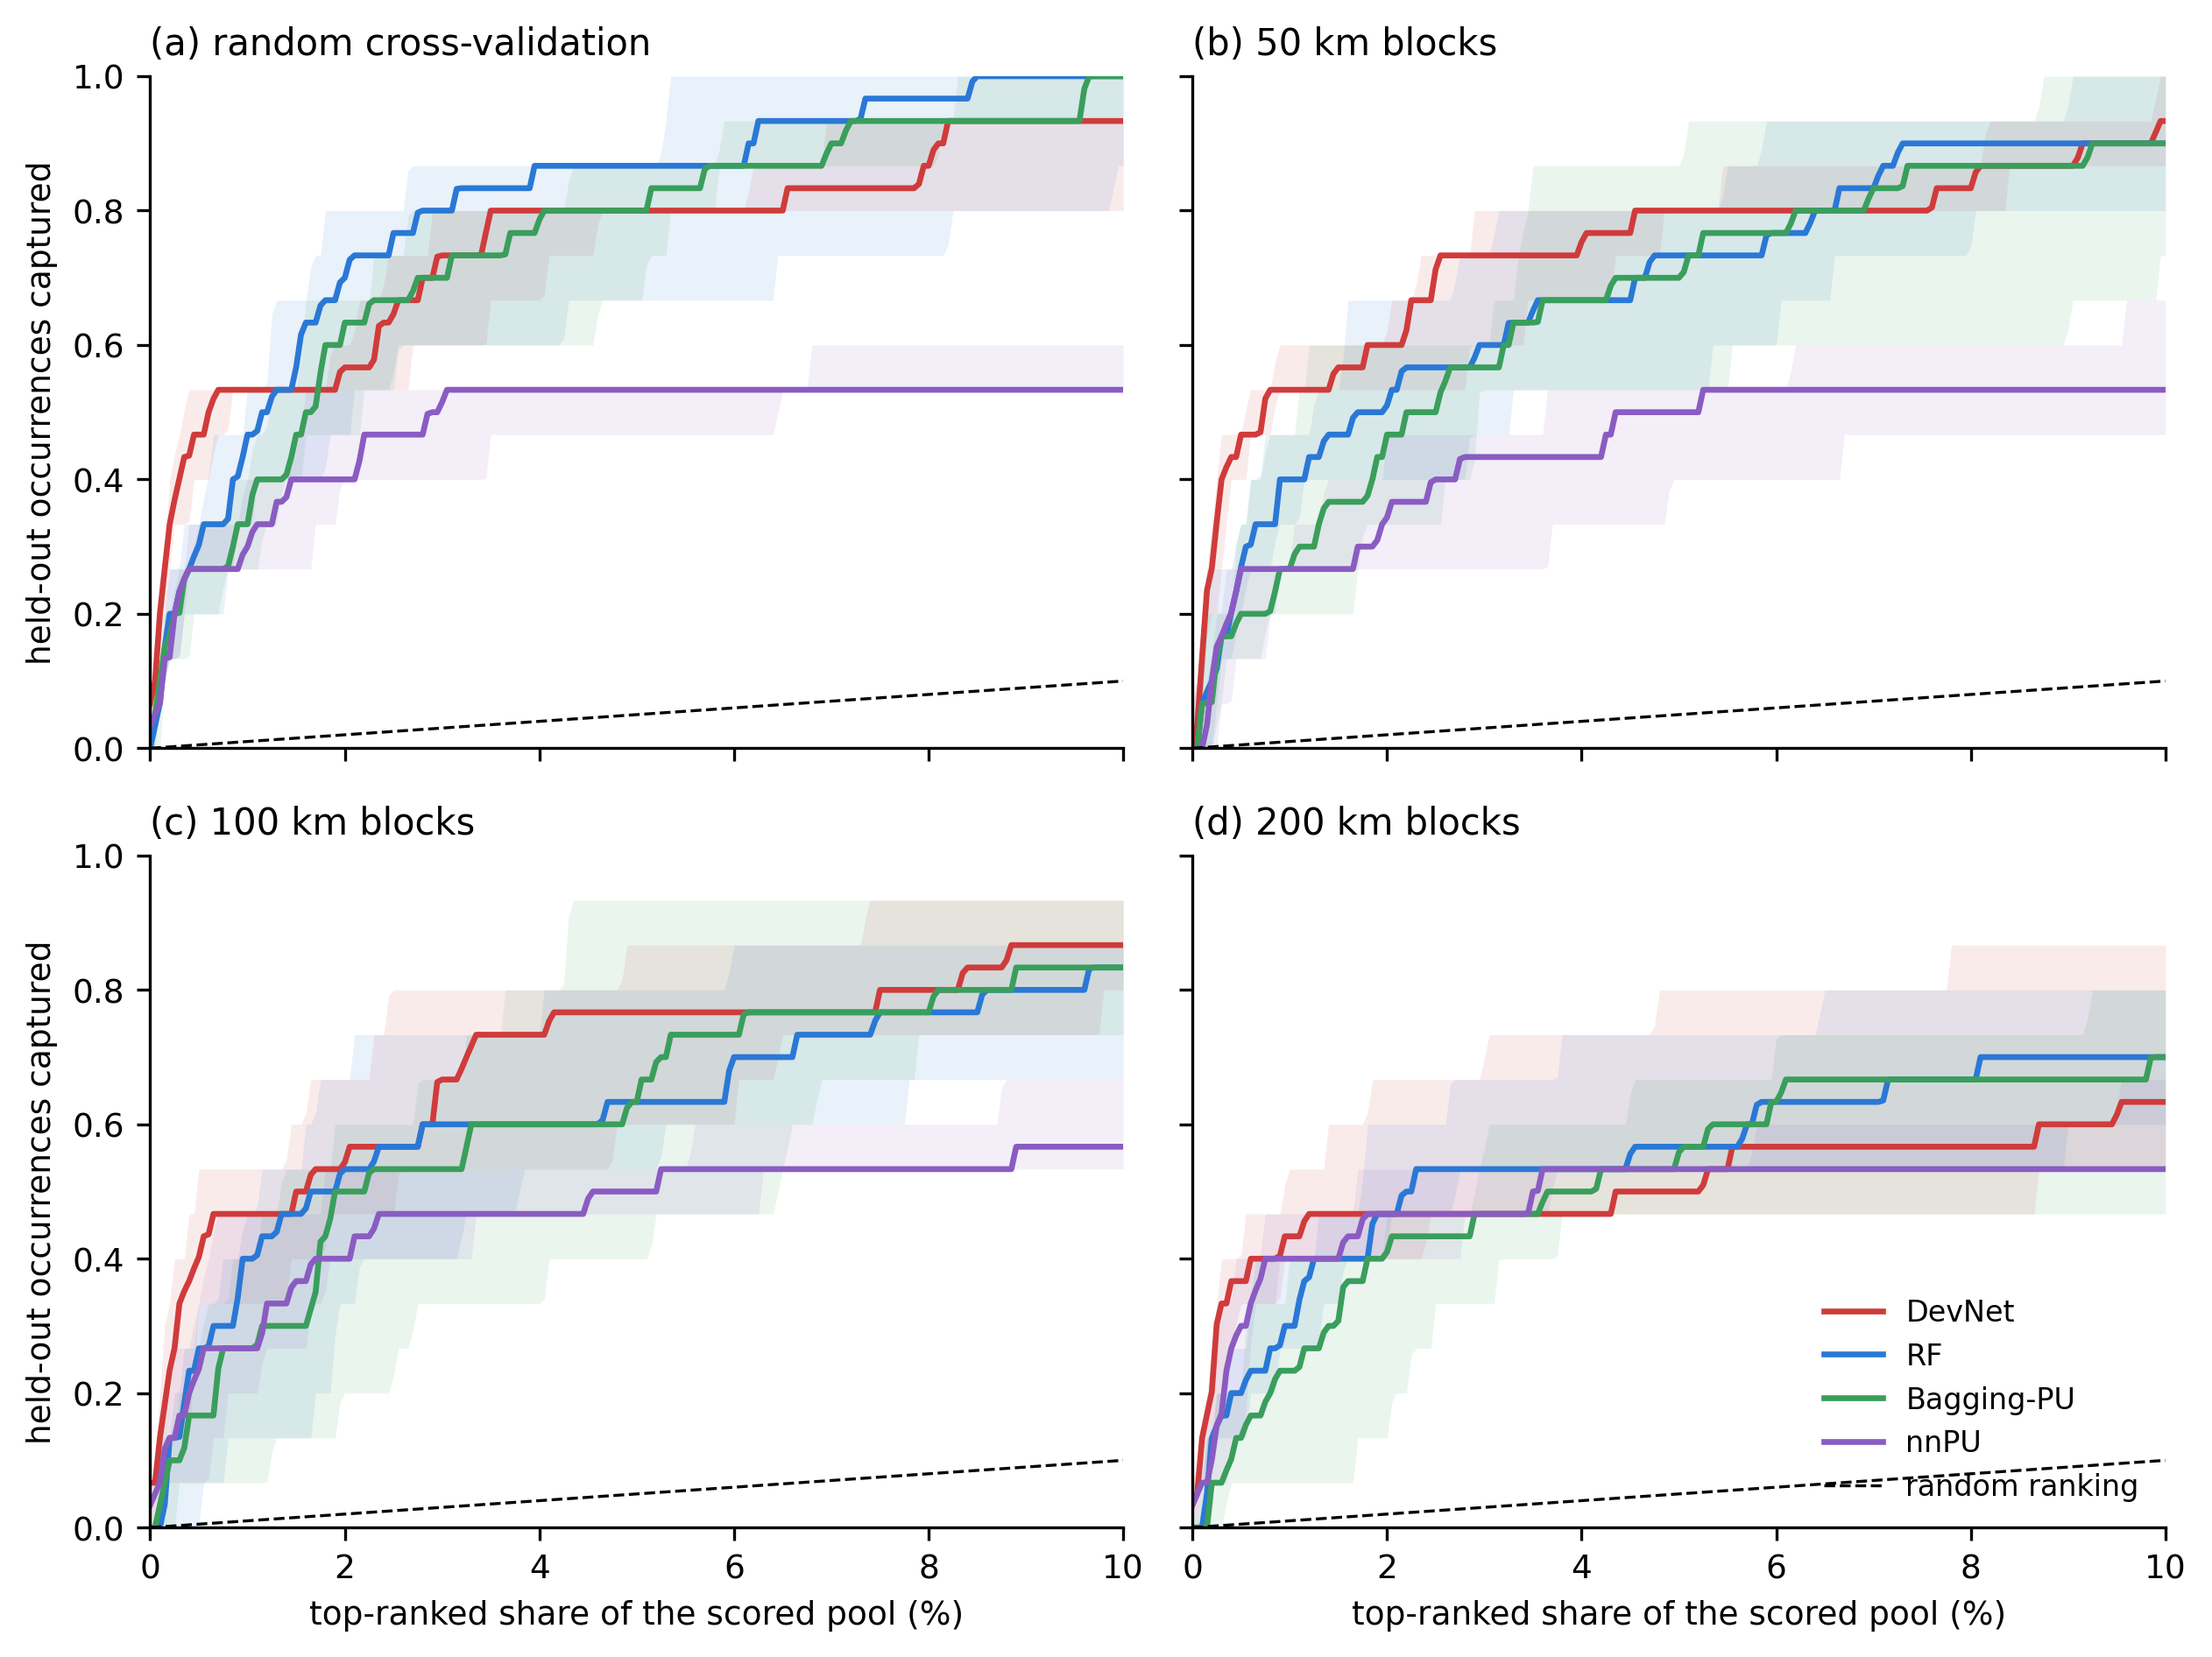
\includegraphics[width=0.92\textwidth]{figures/fig_capture_superior_r4.png}
\caption{Superior capture-rate curves: share of held-out occurrences ranked within the top fraction of the scored pool (a proxy for search area) under (a) random cross-validation and (b) 50~km, (c) 100~km and (d) 200~km spatial blocks. Lines: median over six repeats; bands: range. Dashed: random ranking.}\label{fig:capture}
\end{figure}

\begin{table}[t]
\caption{Average precision (median over six repeats) under random and spatially blocked cross-validation. Bold: highest AP in each row. AUC for the same runs is given in Appendix~\ref{app:full} (Table~\ref{tab:spatial-auc}).}\label{tab:spatial}
\footnotesize
\setlength{\tabcolsep}{3pt}
\begin{tabular*}{\textwidth}{@{\extracolsep\fill}llcccc}
\toprule
Region & Split & DevNet & RF & Bagging-PU & nnPU \\
\midrule
\multirow{4}{*}{Superior} & random & \textbf{0.445} & 0.271 & 0.219 & 0.152 \\
 & 50 km & \textbf{0.418} & 0.192 & 0.148 & 0.102 \\
 & 100 km & \textbf{0.343} & 0.168 & 0.129 & 0.157 \\
 & 200 km & \textbf{0.252} & 0.151 & 0.090 & 0.142 \\
\midrule
\multirow{4}{*}{Cordillera} & random & 0.341 & 0.427 & \textbf{0.433} & 0.022 \\
 & 50 km & \textbf{0.129} & 0.092 & 0.112 & 0.023 \\
 & 100 km & \textbf{0.055} & 0.046 & 0.049 & 0.026 \\
 & 200 km & \textbf{0.076} & 0.039 & 0.038 & 0.019 \\
\midrule
\multirow{4}{*}{Grenville} & random & 0.125 & \textbf{0.257} & 0.191 & 0.008 \\
 & 50 km & 0.031 & \textbf{0.086} & 0.053 & 0.008 \\
 & 100 km & 0.007 & 0.008 & \textbf{0.009} & 0.008 \\
 & 200 km & 0.005 & 0.006 & 0.007 & \textbf{0.008} \\
\botrule
\end{tabular*}
\end{table}

\begin{table}[t]
\caption{Paired comparisons of DevNet with each other model under spatially blocked cross-validation, Superior: difference in AP on repeat-averaged ranks with 95\% bootstrap interval, and the number of the six repeats in which DevNet has the higher AP.}\label{tab:spatial-boot}
\footnotesize
\begin{tabular*}{\textwidth}{@{\extracolsep\fill}llcc}
\toprule
Blocks & Comparison & $\Delta$AP [95\%] & AP wins \\
\midrule
50 km & DevNet $-$ RF & +0.240 [-0.004, +0.475] & 6/6 \\
50 km & DevNet $-$ Bagging-PU & +0.328 [+0.084, +0.553] & 6/6 \\
50 km & DevNet $-$ nnPU & +0.410 [+0.200, +0.577] & 6/6 \\
\addlinespace
100 km & DevNet $-$ RF & +0.196 [+0.011, +0.368] & 6/6 \\
100 km & DevNet $-$ Bagging-PU & +0.245 [+0.014, +0.463] & 6/6 \\
100 km & DevNet $-$ nnPU & +0.188 [+0.050, +0.354] & 6/6 \\
\addlinespace
200 km & DevNet $-$ RF & +0.183 [+0.004, +0.316] & 6/6 \\
200 km & DevNet $-$ Bagging-PU & +0.284 [+0.057, +0.478] & 6/6 \\
200 km & DevNet $-$ nnPU & +0.216 [+0.040, +0.349] & 6/6 \\
\botrule
\end{tabular*}
\end{table}

\subsection{Geological map classes}\label{sec:res-featuresets}

A single map class carries much of the skill in Superior. Removing the alkalic-intrusion column lowers DevNet's AP to 0.345, 0.256, 0.219 and 0.154 under random splits and 50, 100 and 200~km blocks, and RF's to 0.230, 0.126, 0.096 and 0.084: this one class, which covers 6 of the 15 Superior occurrences and 0.5\% of the background, accounts for over a third of DevNet's spatially blocked AP. DevNet without it still has a higher AP than RF with it at every block size. Withholding all point-level map classes costs DevNet and RF about half or more of their AP: DevNet's falls to 0.183 under random splits and 0.133, 0.109 and 0.079 under blocks, RF's to 0.138 and 0.084, 0.069 and 0.051. Without map classes DevNet still has the highest AP under every block size, narrowly ahead of bagging-PU (0.130, 0.079 and 0.065), while bagging-PU leads under random splits (0.225) and nnPU fails (AP 0.007).

\subsection{Tuned baselines and design selection}\label{sec:res-controls}

Tuning did not help the tree-based learners in Superior (Table~\ref{tab:controls}). RF-tuned reached an AP of 0.263, 0.163, 0.142 and 0.117 under random splits and 50, 100 and 200~km blocks, and HGB-tuned 0.200, 0.118, 0.087 and 0.063, at or below the default RF; DevNet had the higher AP than both in all six repeats under every protocol. In Cordillera, HGB-tuned has the highest random-split AP (0.470) and in Grenville the default RF (0.257); under blocks all models are close to chance in both provinces.

DevNet's own design selection carries some optimism (Appendix~\ref{app:full}, Table~\ref{tab:nested}). Choosing the input transformation and batch composition inside each outer training fold gave Superior APs of 0.354, 0.335, 0.312 and 0.190, against 0.445, 0.418, 0.343 and 0.252 for the final configuration, so part of the final configuration's advantage reflects having been chosen with these provinces in view. The nested procedure nevertheless still had the higher AP than RF in 23 of 24 repeat--protocol combinations in Superior.

\begin{table}[t]
\caption{Tuned tree-based baselines: AP (median over six repeats). RF and HGB (tuned): hyperparameters chosen inside each outer training fold by inner 100~km spatial cross-validation. Bold: highest AP in each row.}\label{tab:controls}
\footnotesize
\setlength{\tabcolsep}{3pt}
\begin{tabular*}{\textwidth}{@{\extracolsep\fill}llcccc}
\toprule
Region & Split & DevNet & RF & RF (tuned) & HGB (tuned) \\
\midrule
\multirow{4}{*}{Superior} & random & \textbf{0.445} & 0.271 & 0.263 & 0.200 \\
 & 50 km & \textbf{0.418} & 0.192 & 0.163 & 0.118 \\
 & 100 km & \textbf{0.343} & 0.168 & 0.142 & 0.087 \\
 & 200 km & \textbf{0.252} & 0.151 & 0.117 & 0.063 \\
\midrule
\multirow{4}{*}{Cordillera} & random & 0.341 & 0.427 & 0.435 & \textbf{0.470} \\
 & 50 km & \textbf{0.129} & 0.092 & 0.110 & 0.101 \\
 & 100 km & \textbf{0.055} & 0.046 & 0.048 & 0.036 \\
 & 200 km & \textbf{0.076} & 0.039 & 0.036 & 0.037 \\
\midrule
\multirow{4}{*}{Grenville} & random & 0.125 & \textbf{0.257} & 0.164 & 0.203 \\
 & 50 km & 0.031 & 0.086 & 0.067 & \textbf{0.097} \\
 & 100 km & 0.007 & 0.008 & \textbf{0.009} & 0.006 \\
 & 200 km & 0.005 & \textbf{0.006} & 0.005 & 0.006 \\
\botrule
\end{tabular*}
\end{table}

\subsection{Ablation: what the deviation loss adds}\label{sec:res-ablation}

With all labels, replacing DevNet's deviation loss by cross-entropy changes little (Table~\ref{tab:loss-ablation}). With the map classes DevNet-BCE has a similar or slightly higher AP than DevNet under every protocol (paired differences $-0.056$ to $-0.013$; DevNet higher in at most three of six repeats). Without the map classes DevNet is ahead in 23 of the 24 repeat--protocol combinations, by up to 0.05. DevNet's lead over the tree-based and PU learners therefore comes mainly from its other two components, rank-normal inputs and background-heavy batches (Appendix~\ref{app:sensitivity}): DevNet-BCE, which keeps them, is ahead of RF, bagging-PU and nnPU by similar margins.

The three tests of the semi-supervised premise (Table~\ref{tab:semisup}; Fig.~\ref{fig:semisup}) give a clear but conditional answer. Labelling ground near the occurrences as barren (E1) hurt the model that treats the background as barren more than its unlabelled-background counterpart in most comparisons. In Superior, adding 50 near-occurrence points per occurrence lowered RF's AP from 0.259 to 0.136 but bagging-PU's only from 0.211 to 0.193 (bagging-PU lost less in 18 of 20 repeats); in Cordillera DevNet-BCE lost more than DevNet in 17 of 20 repeats, and in Grenville both DevNet-BCE and RF lost more than their counterparts (17 and 18 of 20). Over the three provinces, with and without map classes, the unlabelled-background model of each pair lost less in five of six comparisons and clearly more in none. With one to three training positives (E3), DevNet was ahead of DevNet-BCE without map classes in Superior at every label count (19 of 20 repeats on average over $k = 1$--3, and 15--20 of 20 at each $k$) and in Grenville (17 of 20); with the map classes the two losses were level. The size of the unlabelled pool (E2) made no consistent difference, contrary to our prediction. Under 100~km blocks in Cordillera and Grenville, where every model is close to chance, all effects are near zero.

\begin{table}[t]
\caption{Ablation of the deviation loss, Superior, all labels: AP (median over six repeats) of DevNet and of DevNet-BCE (identical network, inputs, batches and training; binary cross-entropy with the background labelled 0), and the paired difference on repeat-averaged ranks with 95\% bootstrap interval and the number of repeats in which DevNet has the higher AP. Without map classes: the lithology, era and contact columns removed.}\label{tab:loss-ablation}
\footnotesize
\setlength{\tabcolsep}{3pt}
\begin{tabular*}{\textwidth}{@{\extracolsep\fill}llcccc}
\toprule
Inputs & Split & DevNet & DevNet-BCE & $\Delta$AP [95\%] & wins \\
\midrule
\multirow{4}{*}{Feature set 3} & random & 0.445 & 0.433 & -0.034 [-0.086, -0.001] & 3/6 \\
 & 50 km & 0.418 & 0.434 & -0.034 [-0.095, +0.004] & 0/6 \\
 & 100 km & 0.343 & 0.346 & -0.056 [-0.126, +0.011] & 1/6 \\
 & 200 km & 0.252 & 0.233 & -0.013 [-0.062, +0.017] & 2/6 \\
\midrule
\multirow{4}{*}{Without map classes} & random & 0.183 & 0.157 & +0.017 [-0.150, +0.237] & 6/6 \\
 & 50 km & 0.133 & 0.094 & +0.021 [-0.111, +0.220] & 6/6 \\
 & 100 km & 0.109 & 0.088 & -0.010 [-0.135, +0.145] & 5/6 \\
 & 200 km & 0.079 & 0.050 & +0.053 [-0.040, +0.227] & 6/6 \\
\botrule
\end{tabular*}
\end{table}

\begin{table}[t]
\caption{Tests of the semi-supervised premise (random cross-validation, 20 repeats). Each entry is the median effect in favour of the model that treats the background as unlabelled (DevNet, bagging-PU), with the number of the 20 repeats in which it is positive. Mislabelled ground: the AP change of the unlabelled-background model minus that of its counterpart when 50 points per occurrence from a 2--10~km annulus are added to the training background. Few labels: the AP difference averaged over one to three training positives per fold.}\label{tab:semisup}
\footnotesize
\setlength{\tabcolsep}{3pt}
\begin{tabular*}{\textwidth}{@{\extracolsep\fill}p{2.6cm}p{3.2cm}ccc}
\toprule
Test & Pair & Superior & Cordillera & Grenville \\
\midrule
Ground near occurrences labelled barren & DevNet vs DevNet-BCE & +0.003 (12/20) & +0.025 (17/20) & +0.044 (17/20) \\
 & Bagging-PU vs RF & +0.089 (18/20) & +0.030 (11/20) & +0.130 (18/20) \\
One to three training positives & DevNet vs DevNet-BCE & -0.001 (8/20) & +0.004 (16/20) & +0.001 (13/20) \\
 & DevNet vs DevNet-BCE, without map classes & +0.034 (19/20) & +0.003 (12/20) & +0.011 (17/20) \\
\botrule
\end{tabular*}
\end{table}

\begin{figure}[t]
\centering
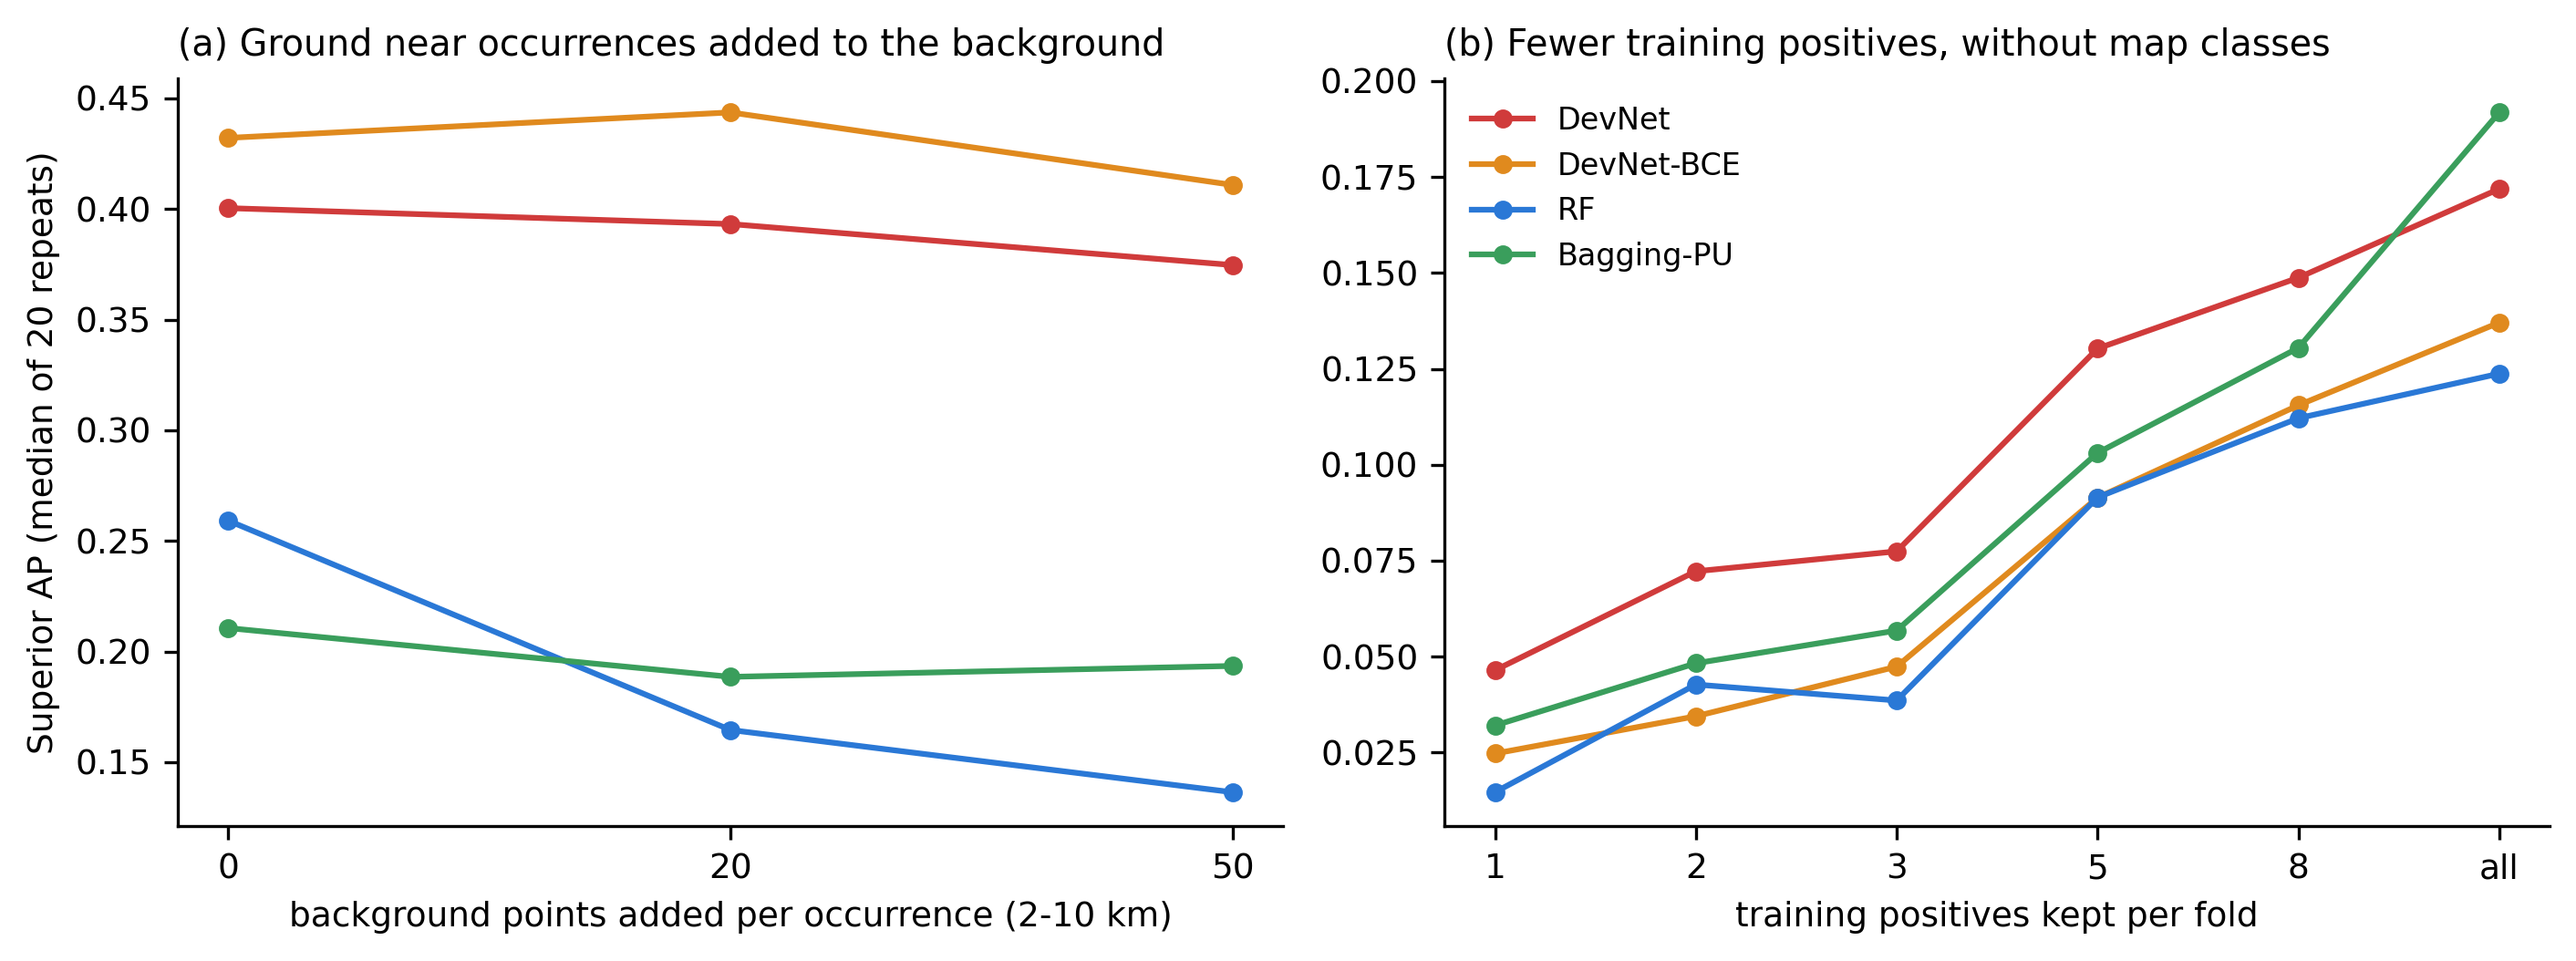
\includegraphics[width=\textwidth]{figures/fig_semisup_r4.png}
\caption{Tests of the semi-supervised premise, Superior, random cross-validation (median AP over 20 repeats): (a) background points added in a 2--10~km annulus around each occurrence; (b) training positives kept per fold, without the point-level map classes.}\label{fig:semisup}
\end{figure}

\subsection{How much of the score is location?}\label{sec:res-geography}

A random forest given only coordinates reaches an AP of 0.507 in Cordillera under random cross-validation, higher than any evidence-based model (at most 0.470, HGB-tuned), and 0.249 in Grenville, about as high as the best of them (RF, 0.257; Table~\ref{tab:geography}). In these two provinces the random-split skill of the tree-based models can therefore be reproduced without any geology: training occurrences cluster, a random split leaves most held-out occurrences close to a training occurrence, and a flexible learner can exploit that proximity, through the coordinates themselves or through spatially smooth layers that act as surrogate coordinates. Under 100~km blocks the coordinate-only model collapses (0.052 and 0.075), as do the evidence-based models ($\leq 0.062$ and $\leq 0.009$).

Superior is the exception. Coordinates alone reach only 0.157 under random splits and 0.018 under blocking, far below every evidence-based model except nnPU, so the Superior scores reflect a signature in the evidence rather than location. DevNet uses the evidence better than an L2-regularised logistic regression in every province (random splits: 0.445, 0.341 and 0.125 against 0.374, 0.210 and 0.037; 100~km blocks in Superior: 0.343 against 0.219).

\begin{table}[t]
\caption{Geography-only and linear baselines: AP and AUC (median over six repeats) under random cross-validation and 100~km spatial blocks, on identical folds. RF, coordinates only: random forest trained on projected coordinates without any evidence layer.}\label{tab:geography}
\footnotesize
\setlength{\tabcolsep}{3pt}
\begin{tabular*}{\textwidth}{@{\extracolsep\fill}llcccc}
\toprule
 & & \multicolumn{2}{c}{Random CV} & \multicolumn{2}{c}{100 km blocks} \\
\cmidrule(lr){3-4}\cmidrule(lr){5-6}
Region & Model & AP & AUC & AP & AUC \\
\midrule
\multirow{4}{*}{Superior} & RF, coordinates only & 0.157 & 0.782 & 0.018 & 0.750 \\
 & RF, all features & 0.271 & 0.983 & 0.168 & 0.904 \\
 & Logistic regression & 0.374 & 0.924 & 0.219 & 0.942 \\
 & DevNet & 0.445 & 0.972 & 0.343 & 0.950 \\
\midrule
\multirow{4}{*}{Cordillera} & RF, coordinates only & 0.507 & 0.922 & 0.052 & 0.727 \\
 & RF, all features & 0.427 & 0.931 & 0.046 & 0.776 \\
 & Logistic regression & 0.210 & 0.916 & 0.062 & 0.826 \\
 & DevNet & 0.341 & 0.914 & 0.055 & 0.790 \\
\midrule
\multirow{4}{*}{Grenville} & RF, coordinates only & 0.249 & 0.821 & 0.075 & 0.750 \\
 & RF, all features & 0.257 & 0.838 & 0.008 & 0.538 \\
 & Logistic regression & 0.037 & 0.766 & 0.005 & 0.624 \\
 & DevNet & 0.125 & 0.799 & 0.007 & 0.661 \\
\botrule
\end{tabular*}
\end{table}

\subsection{Synthetic positives}\label{sec:res-augmentation}

The generators behave very differently (Table~\ref{tab:aug-diag}; Fig.~\ref{fig:aug-pca}). Jitter and SMOTE samples lie close to the real positives (median nearest-neighbour ratio 0.10 and 0.24) and almost all have a real positive as their nearest labelled neighbour (100\% and 97\%): they are near-copies of the training occurrences. WGAN-GP samples are as far from the real positives as the real positives are from one another (ratio 0.91), but for 35\% of them the nearest labelled point is a background point: with 15 training points the generator spreads probability mass into background-like parts of feature space. All three sets of samples receive high DevNet scores (median percentile 0.98).

Because the folds are identical with and without augmentation, the effect is measured as the paired, per-repeat difference in AP (Table~\ref{tab:augmentation}; Fig.~\ref{fig:aug-perf}). For DevNet no generator helps: the median per-repeat change in AP lies between $-0.041$ and $-0.003$, and no configuration raises AP in more than three of the six repeats. For RF, jitter raises AP (median $+0.06$ to $+0.07$, in four or five of six repeats), SMOTE lowers it (by 0.070 at $m = 10$), and WGAN-GP changes it little. The best augmented RF (jitter $10\times$, AP 0.327) remains well below DevNet without augmentation (0.445). Under spatial blocking (Appendix~\ref{app:aug-spatial}, Table~\ref{tab:aug-spatial}) WGAN-GP at $10\times$ raises RF's AP with 100~km blocks from 0.168 to 0.219, still below unaugmented DevNet (0.343), but with 200~km blocks every generator lowers RF's AP or leaves it unchanged. For DevNet the per-repeat changes under blocking are small (medians between $-0.031$ and $+0.001$).

\begin{figure}[t]
\centering
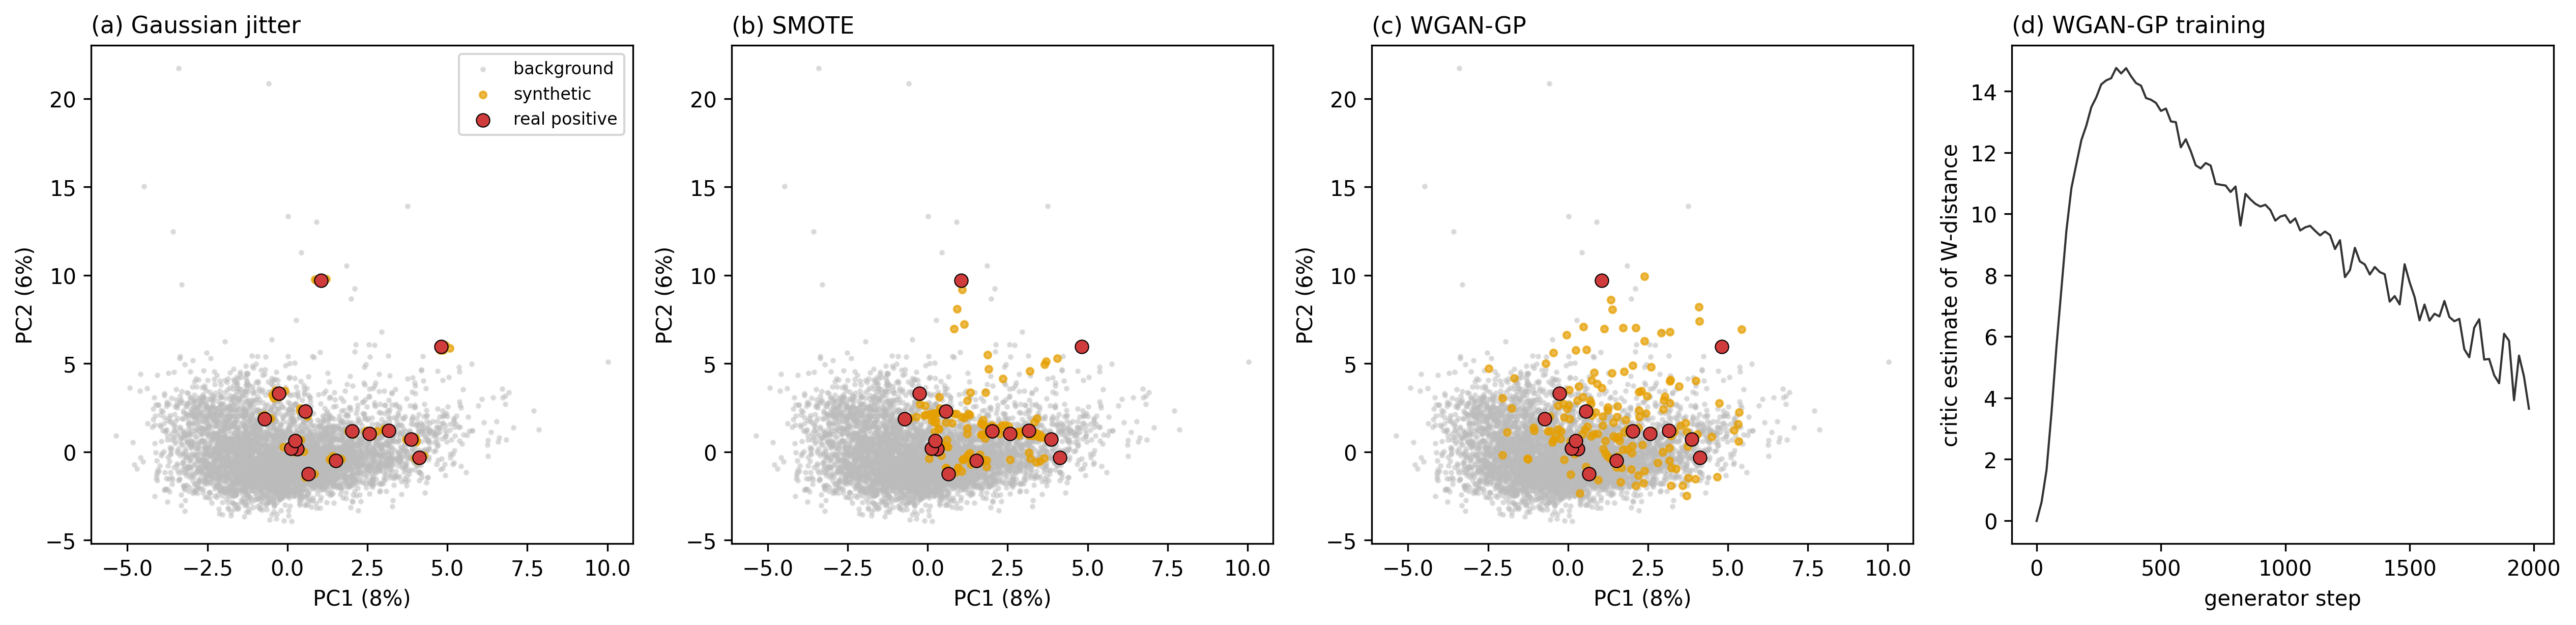
\includegraphics[width=\textwidth]{figures/fig_augmentation_superior_r4.png}
\caption{(a--c) Synthetic positives from each generator (fitted to all 15 Superior positives) in the first two principal components of background and real positives. (d) WGAN-GP critic estimate of the Wasserstein distance during training.}\label{fig:aug-pca}
\end{figure}

\begin{figure}[t]
\centering
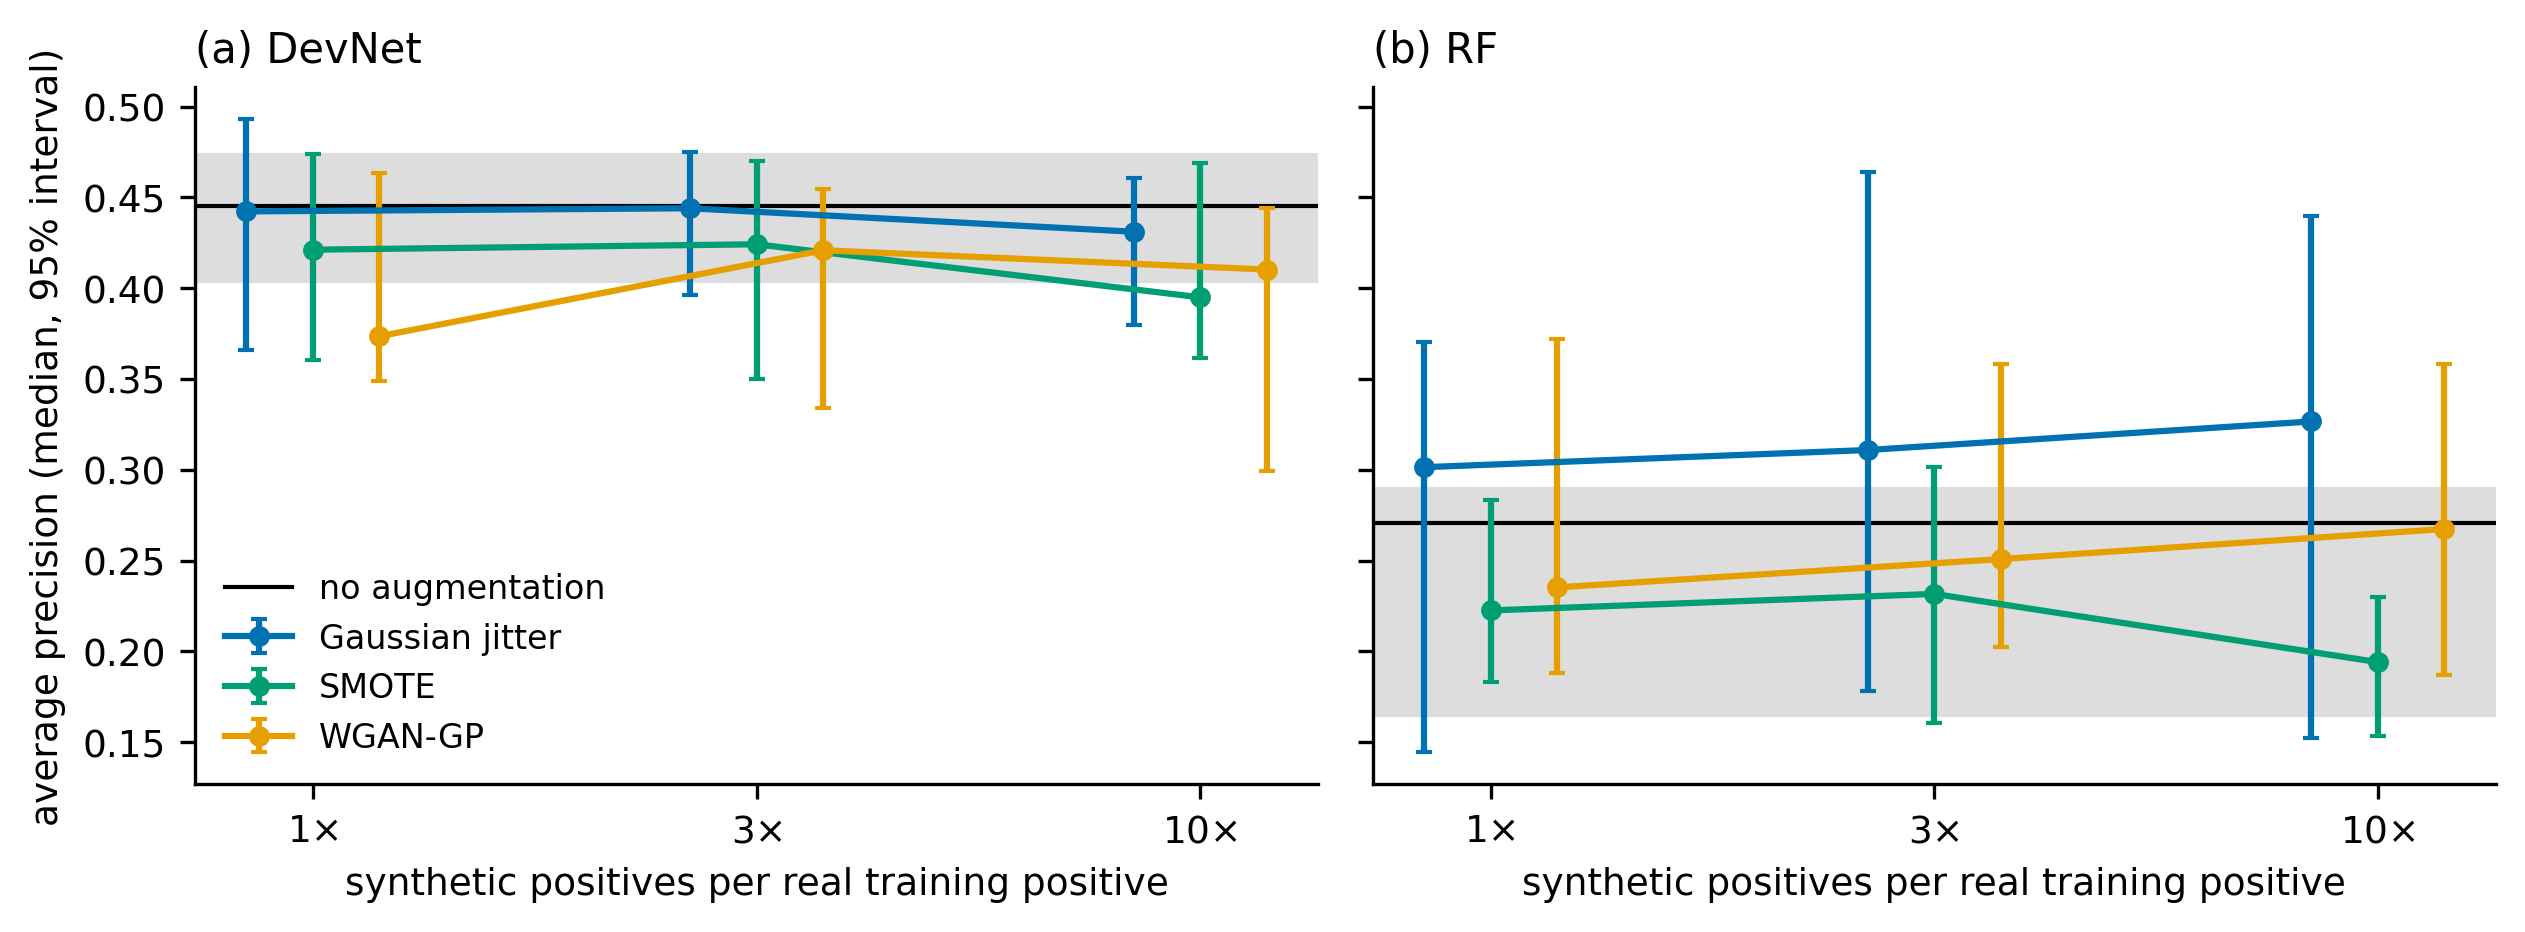
\includegraphics[width=\textwidth]{figures/fig_augmentation_performance_r4.png}
\caption{Superior average precision with fold-safe synthetic positives, by generator and number of synthetic positives per real training positive. Line and grey band: no augmentation (median and 95\% interval).}\label{fig:aug-perf}
\end{figure}

\begin{table}[t]
\caption{Effect of fold-safe positive augmentation on held-out performance, Superior (random cross-validation, identical folds; held-out positives always real). $\Delta$AP: paired difference from no augmentation in each of the six repeats (median [min, max]); wins: repeats with higher AP than without augmentation.}\label{tab:augmentation}
\scriptsize
\setlength{\tabcolsep}{2.5pt}
\begin{tabular*}{\textwidth}{@{\extracolsep\fill}lllcccc}
\toprule
Model & Generator & $m$ & AUC & AP & $\Delta$AP per repeat & wins \\
\midrule
\multirow{10}{*}{DevNet} & none & -- & 0.972 & 0.445 [0.404, 0.474] & -- & -- \\
 & Gaussian jitter & 1$\times$ & 0.964 & 0.442 [0.366, 0.493] & -0.003 [-0.093, +0.025] & 2/6 \\
 & Gaussian jitter & 3$\times$ & 0.973 & 0.444 [0.396, 0.475] & -0.006 [-0.009, +0.021] & 2/6 \\
 & Gaussian jitter & 10$\times$ & 0.974 & 0.431 [0.380, 0.461] & -0.008 [-0.078, +0.004] & 1/6 \\
 & SMOTE & 1$\times$ & 0.974 & 0.421 [0.360, 0.474] & -0.025 [-0.045, +0.020] & 1/6 \\
 & SMOTE & 3$\times$ & 0.972 & 0.424 [0.350, 0.470] & -0.017 [-0.056, +0.000] & 1/6 \\
 & SMOTE & 10$\times$ & 0.975 & 0.395 [0.362, 0.469] & -0.035 [-0.097, +0.013] & 2/6 \\
 & WGAN-GP & 1$\times$ & 0.968 & 0.374 [0.349, 0.464] & -0.041 [-0.109, +0.010] & 1/6 \\
 & WGAN-GP & 3$\times$ & 0.970 & 0.421 [0.334, 0.454] & -0.016 [-0.123, +0.029] & 3/6 \\
 & WGAN-GP & 10$\times$ & 0.964 & 0.410 [0.299, 0.444] & -0.025 [-0.170, -0.005] & 0/6 \\
\midrule
\multirow{10}{*}{RF} & none & -- & 0.983 & 0.271 [0.165, 0.289] & -- & -- \\
 & Gaussian jitter & 1$\times$ & 0.973 & 0.301 [0.144, 0.371] & +0.059 [-0.065, +0.083] & 4/6 \\
 & Gaussian jitter & 3$\times$ & 0.983 & 0.311 [0.178, 0.464] & +0.059 [-0.071, +0.211] & 5/6 \\
 & Gaussian jitter & 10$\times$ & 0.975 & 0.327 [0.152, 0.440] & +0.069 [-0.042, +0.159] & 4/6 \\
 & SMOTE & 1$\times$ & 0.980 & 0.223 [0.183, 0.283] & -0.021 [-0.066, +0.022] & 2/6 \\
 & SMOTE & 3$\times$ & 0.984 & 0.232 [0.161, 0.301] & -0.006 [-0.078, +0.027] & 2/6 \\
 & SMOTE & 10$\times$ & 0.981 & 0.194 [0.154, 0.230] & -0.070 [-0.113, +0.002] & 1/6 \\
 & WGAN-GP & 1$\times$ & 0.963 & 0.235 [0.188, 0.372] & +0.007 [-0.100, +0.098] & 3/6 \\
 & WGAN-GP & 3$\times$ & 0.979 & 0.251 [0.202, 0.358] & +0.018 [-0.066, +0.132] & 3/6 \\
 & WGAN-GP & 10$\times$ & 0.985 & 0.267 [0.187, 0.358] & +0.035 [-0.079, +0.115] & 4/6 \\
\botrule
\end{tabular*}
\end{table}

\begin{table}[t]
\caption{What the generators produce (fitted to all 15 Superior positives; 150 samples each). NN ratio: distance to the nearest real positive divided by the median nearest-neighbour distance among real positives (0 = copy). Nearest labelled neighbour: share of samples whose nearest point among positives and training background is a positive. DevNet percentile: median score percentile among the training background under the production DevNet.}\label{tab:aug-diag}
\footnotesize
\setlength{\tabcolsep}{2.5pt}
\begin{tabular*}{\textwidth}{@{\extracolsep\fill}lcccc}
\toprule
Source & NN ratio, median & NN ratio, P10 & NN is positive & DevNet pct. \\
\midrule
Real occurrences (leave-one-out) & 1.00 & 0.55 & -- & 0.995 \\
Gaussian jitter & 0.10 & 0.08 & 100\% & 0.984 \\
SMOTE & 0.24 & 0.06 & 97\% & 0.982 \\
WGAN-GP & 0.91 & 0.58 & 65\% & 0.985 \\
Background (300 random points) & 1.51 & -- & -- & 0.500 \\
\botrule
\end{tabular*}
\end{table}

\subsection{Validation-protocol audit}\label{sec:res-audit}

Rebuilding the S2 parent--child augmentation and child-level random splitting of \citet{Parsa2024} on our data gives a test AUC of 0.999--1.000 in all three provinces and for both negative-sampling rules (Table~\ref{tab:audit}; Fig.~\ref{fig:audit}). In 97--99\% of the test positives, at least one sibling child cell of the same occurrence is in the training set. In feature space, siblings are closer to each other (median standardised distance 2.5--3.9) than occurrences are to their nearest other occurrence (4.3--7.1) and than background points are to their nearest background neighbour (4.6--4.9; Table~\ref{tab:audit-sim}), because the coarse deep-architecture layers and the map classes take identical values in sibling cells and the fine-scale layers nearly so.

The honest reference within this balanced 70/30 design is one label per occurrence with random negatives. It gives a mean AUC of 0.976 in Superior, 0.887 in Cordillera and 0.767 in Grenville, each with a wide range over the 50 splits (0.80--1.00, 0.75--1.00 and 0.50--1.00). The child-level split therefore inflates test AUC by about 0.02, 0.11 and 0.23 respectively, the inflation being largest where real skill is lowest, and it collapses the apparent uncertainty to almost nothing. Drawing negatives from the least similar 5\% of the ground inflates AUC independently of the split: without augmentation, cosine-dissimilar negatives raise mean AUC to 0.999, 0.997 and 1.000. Keeping all children of one parent on the same side of the split removes most, but not all, of the augmentation effect (Superior 0.972, Cordillera 0.961, Grenville 0.905 with random negatives); the remainder reflects the fourfold larger training set and spatial dependence between neighbouring occurrences in different parent cells, which only spatial blocking removes.

\begin{figure}[t]
\centering
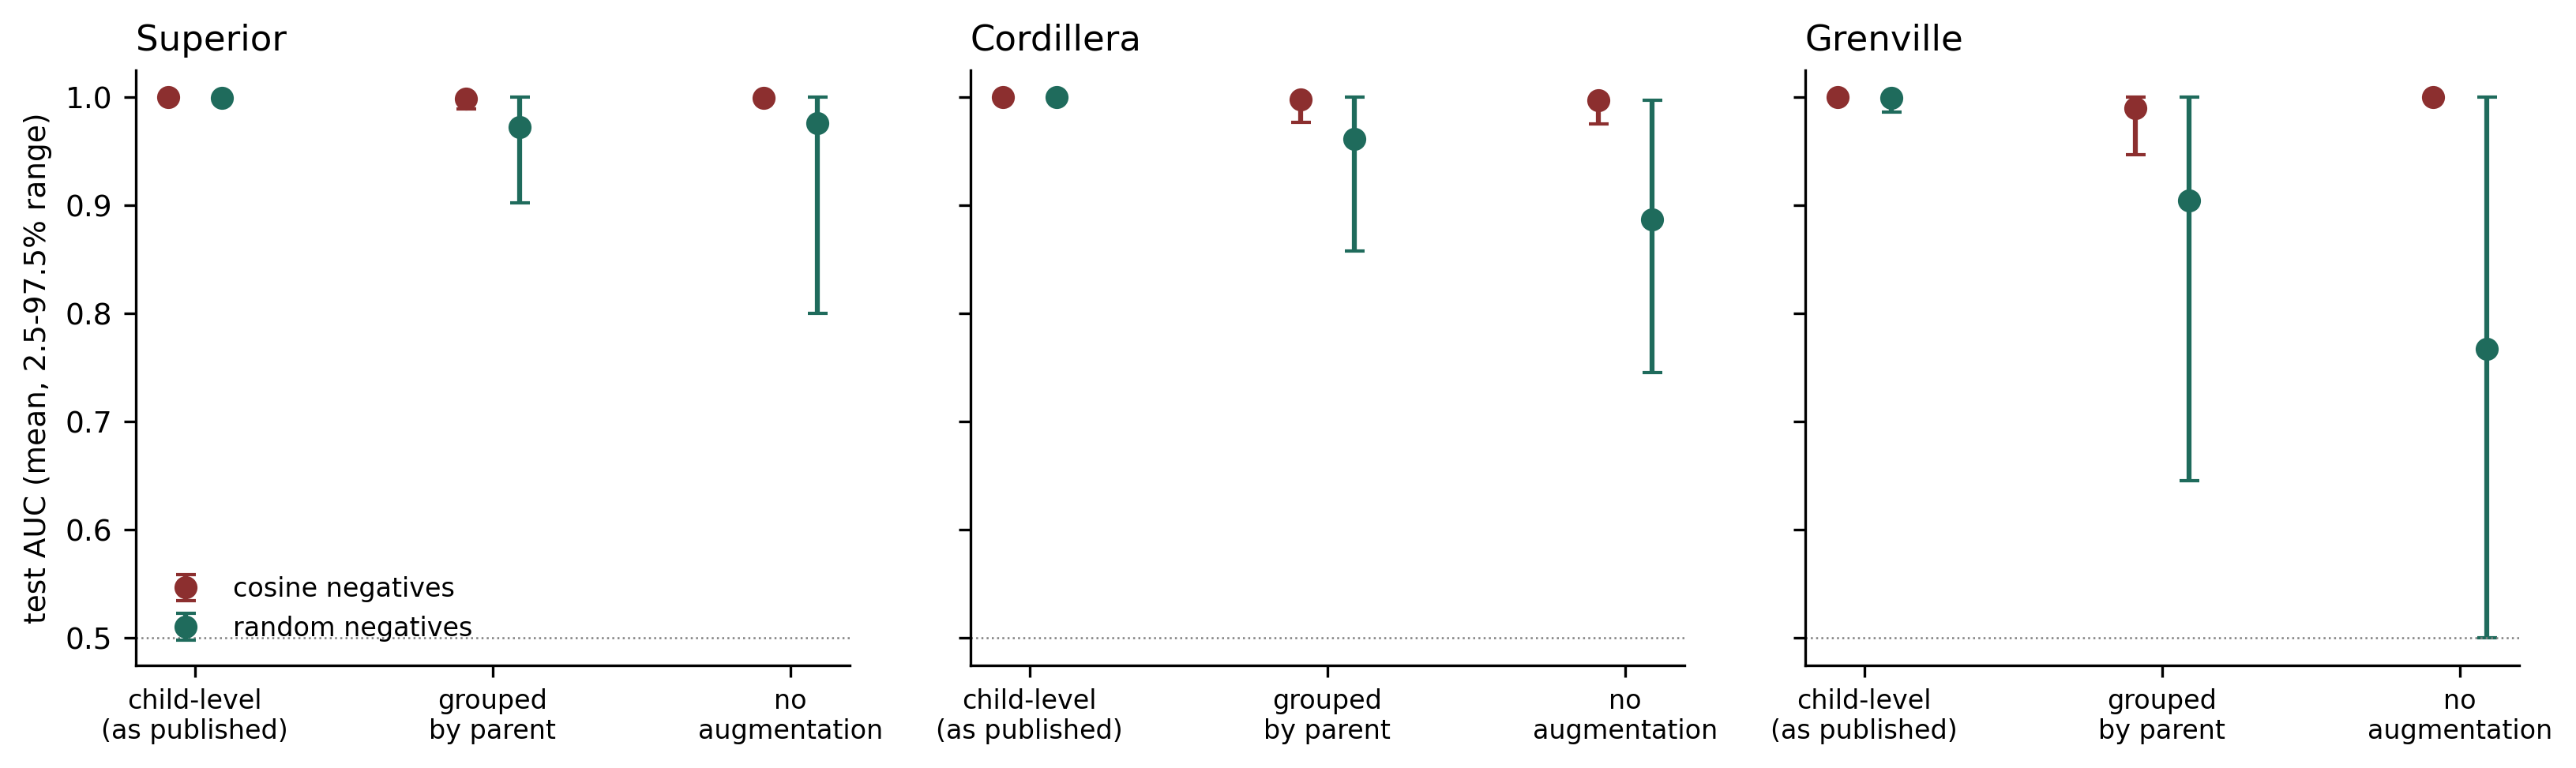
\includegraphics[width=\textwidth]{figures/fig_protocol_audit_r4.png}
\caption{Protocol audit: random forest test AUC under S2 parent--child augmentation for three split designs and two negative-sampling rules (mean and 2.5--97.5 percentile range over 50 balanced 70/30 splits).}\label{fig:audit}
\end{figure}

\begin{table}[t]
\caption{Feature-space distance (median, standardised features) between sibling child cells of the same occurrence, from each occurrence to its nearest other occurrence, and from background points to their nearest background neighbour.}\label{tab:audit-sim}
\footnotesize
\begin{tabular*}{0.8\textwidth}{@{\extracolsep\fill}lccc}
\toprule
Region & Siblings & Nearest other occurrence & Nearest background neighbour \\
\midrule
Superior & 3.89 & 5.36 & 4.59 \\
Cordillera & 2.53 & 4.29 & 4.68 \\
Grenville & 3.25 & 7.09 & 4.90 \\
\botrule
\end{tabular*}
\end{table}

\begin{table}[t]
\caption{Protocol audit: random forest test AUC (mean and 2.5--97.5 percentile range over 50 stratified 70/30 splits of balanced labels) under the S2 parent--child augmentation of \citet{Parsa2024}, for two negative-sampling rules (cosine-dissimilar or random) and three split designs (child-level random, as published; children grouped by parent; no augmentation). Pos.: positive labels. Sibling: share of test positives with a sibling child cell in the training set.}\label{tab:audit}
\scriptsize
\setlength{\tabcolsep}{2.5pt}
\begin{tabular*}{\textwidth}{@{\extracolsep\fill}lllccc}
\toprule
Region & Negatives & Split & Pos. & Test AUC & Sibling \\
\midrule
\multirow{6}{*}{Superior} & cosine & child-level & 60 & 1.000 [1.000, 1.000] & 98\% \\
 & cosine & parent-grouped & 60 & 0.999 [0.989, 1.000] & -- \\
 & cosine & no augm. & 15 & 0.999 [1.000, 1.000] & -- \\
 & random & child-level & 60 & 0.999 [0.995, 1.000] & 98\% \\
 & random & parent-grouped & 60 & 0.972 [0.902, 1.000] & -- \\
 & random & no augm. & 15 & 0.976 [0.800, 1.000] & -- \\
\midrule
\multirow{6}{*}{Cordillera} & cosine & child-level & 108 & 1.000 [1.000, 1.000] & 97\% \\
 & cosine & parent-grouped & 108 & 0.998 [0.976, 1.000] & -- \\
 & cosine & no augm. & 27 & 0.997 [0.975, 1.000] & -- \\
 & random & child-level & 108 & 1.000 [0.998, 1.000] & 97\% \\
 & random & parent-grouped & 108 & 0.961 [0.858, 1.000] & -- \\
 & random & no augm. & 27 & 0.887 [0.745, 0.997] & -- \\
\midrule
\multirow{6}{*}{Grenville} & cosine & child-level & 48 & 1.000 [1.000, 1.000] & 99\% \\
 & cosine & parent-grouped & 48 & 0.990 [0.946, 1.000] & -- \\
 & cosine & no augm. & 12 & 1.000 [1.000, 1.000] & -- \\
 & random & child-level & 48 & 0.999 [0.986, 1.000] & 99\% \\
 & random & parent-grouped & 48 & 0.905 [0.646, 1.000] & -- \\
 & random & no augm. & 12 & 0.767 [0.500, 1.000] & -- \\
\botrule
\end{tabular*}
\end{table}

\subsection{Model interpretation}\label{sec:res-shap}

With the rank-based direction rule, RF and DevNet agree on the sign of the effect for all ten of their jointly most important features in each province (Table~\ref{tab:shap}; Appendix~\ref{app:shap}). Read from the sign of the mean SHAP value instead, the two models would appear to disagree on many of these features, an artefact of the two explainers' different baselines (Section~\ref{sec:shap}).

The two models agree on directions but weight the evidence differently (Fig.~\ref{fig:shap}). In Superior, DevNet ranks five geological classes of the cell first: extrusive (greenstone) lithology, an age contact within the cell and alkalic intrusive lithology raise the score, and Archean era and tonalite lower it; it then ranks proximity to regional greenstone, Bouguer GLCM correlation (lower values more prospective) and LAB depth. RF ranks the horizontal-gradient magnitude of deep-source magnetics first (lower values more prospective), then LAB depth, proximity to regional greenstone and fault proximity, and gives the geological classes low ranks (20th--34th of 48). Both models score ground as more prospective where the LAB is shallower, close to greenstone belts and faults, where TMI is high, and farther from deep magnetic worms. In Cordillera both models treat Mesozoic terranes and ground far from high-grade metamorphic units as unfavourable and Proterozoic terranes as favourable. In Grenville both rank deep-source magnetics and distance to regional age contacts among their four most important features, but given the weak predictive skill there these attributions describe the signal the models attempted to use rather than a reliable control.

\begin{figure}[t]
\centering
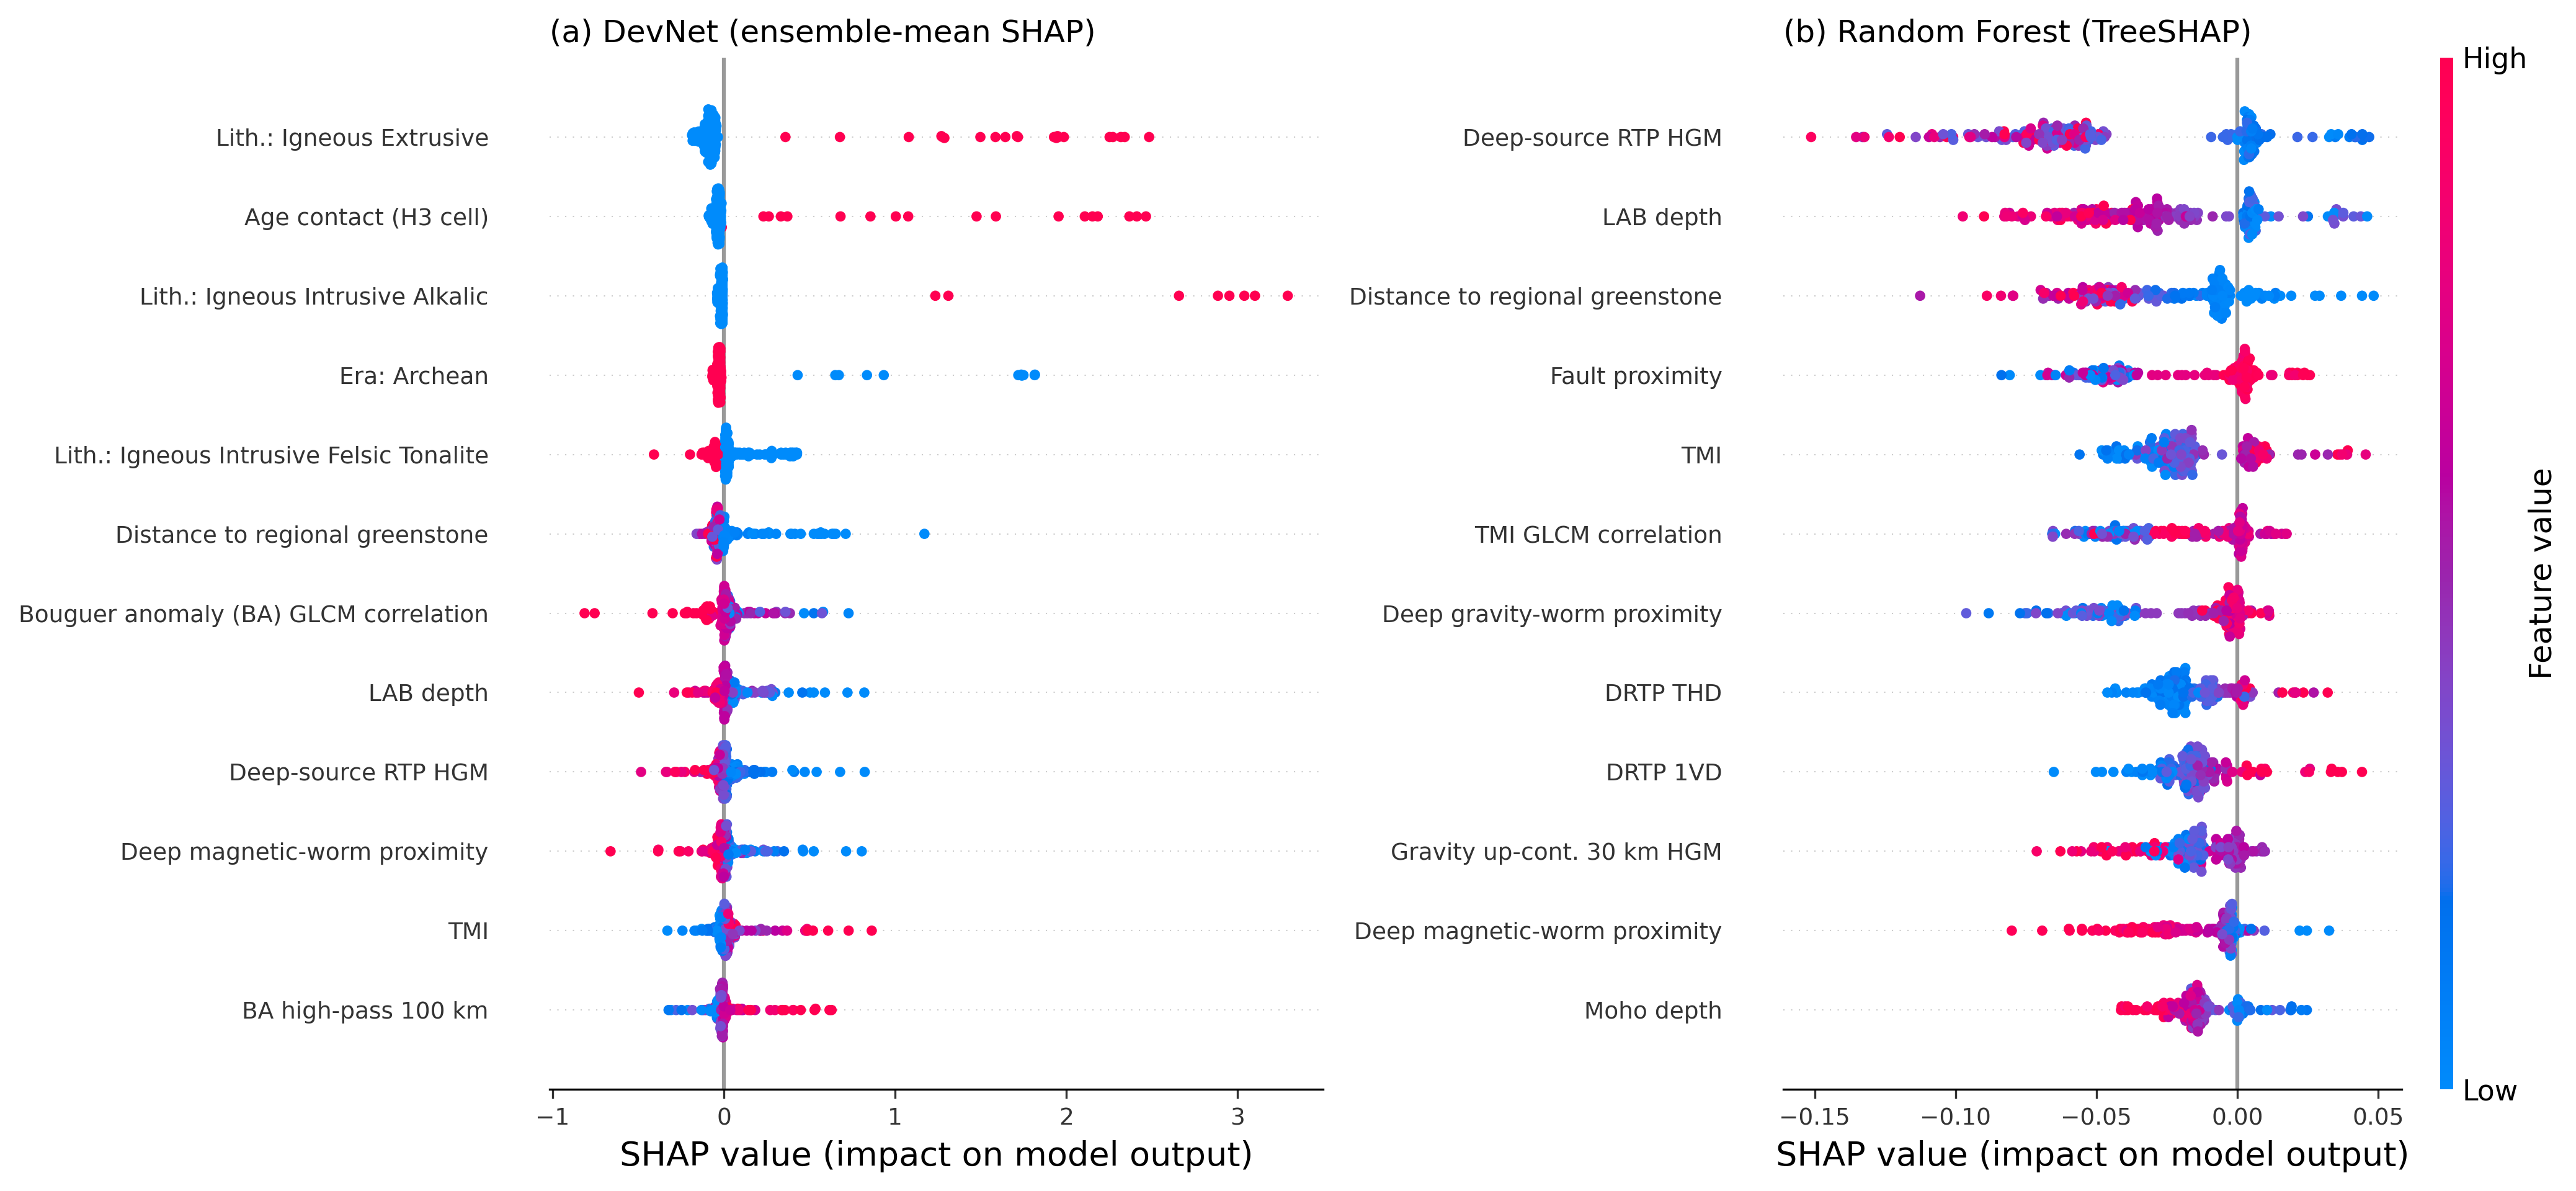
\includegraphics[width=\textwidth]{figures/fig_shap_superior_r2.png}
\caption{SHAP summaries for Superior: (a) DevNet (DeepSHAP on its quantile-transformed inputs, mean over the five ensemble members) and (b) RF (TreeSHAP). Each point is one explained sample; colour is the feature value. SHAP magnitudes are not comparable between models (unbounded anomaly score vs probability).}\label{fig:shap}
\end{figure}

\begin{table}[t]
\caption{Superior: the ten jointly most important features (mean $|$SHAP$|$, normalised per model). Rank among 48 features; direction $\uparrow$/$\downarrow$: higher values (or presence) raise/lower the score, with Spearman $\rho$ between feature value and SHAP value.}\label{tab:shap}
\scriptsize
\setlength{\tabcolsep}{2.5pt}
\begin{tabular*}{\textwidth}{@{\extracolsep\fill}lcccc}
\toprule
Feature & DevNet rank & DevNet dir. & RF rank & RF dir. \\
\midrule
Deep-source RTP HGM & 9 & $\downarrow$ (-0.95) & 1 & $\downarrow$ (-0.74) \\
Lith.: Igneous Extrusive & 1 & $\uparrow$ (+0.53) & 34 & $\uparrow$ (+0.53) \\
LAB depth & 8 & $\downarrow$ (-0.94) & 2 & $\downarrow$ (-0.90) \\
Distance to regional greenstone & 6 & $\downarrow$ (-0.89) & 3 & $\downarrow$ (-0.90) \\
Age contact (H3 cell) & 2 & $\uparrow$ (+0.50) & 31 & $\uparrow$ (+0.50) \\
TMI & 11 & $\uparrow$ (+0.92) & 5 & $\uparrow$ (+0.86) \\
Lith.: Igneous Intrusive Alkalic & 3 & $\uparrow$ (+0.34) & 20 & $\uparrow$ (+0.34) \\
Fault proximity & 15 & $\uparrow$ (+0.90) & 4 & $\uparrow$ (+0.84) \\
Bouguer anomaly (BA) GLCM correlation & 7 & $\downarrow$ (-0.88) & 16 & $\downarrow$ (-0.90) \\
Deep magnetic-worm proximity & 10 & $\downarrow$ (-0.92) & 11 & $\downarrow$ (-0.93) \\
\botrule
\end{tabular*}
\end{table}

\subsection{Prospectivity maps and external checks}\label{sec:res-maps}

The production DevNet and RF maps (Fig.~\ref{fig:maps}) both concentrate their highest classes in the southern Superior Province, around the eastern-Abitibi cluster and across the Abitibi and Wawa subprovinces, but their rankings of the province are only moderately similar (Spearman correlation over the grid 0.37). RF assigns a probability of exactly zero to 83\% of the grid, so its classes are drawn from the remaining nodes. In the Kapuskasing area (Fig.~\ref{fig:ksz}) DevNet places its top 1\% mainly in the Abitibi Subprovince east of the KSZ; along the KSZ itself, the top 5\% and 10\% classes form discontinuous north-north-east trending patches on its western side. Clay-Howells, the untrained Fe--REE--Nb resource on the KSZ, lies 79~km from the nearest training occurrence; among the province's 8,000 random background points the production models place it at the 96.9th (DevNet) and 99.4th (RF) percentile.

\begin{figure}[t]
\centering
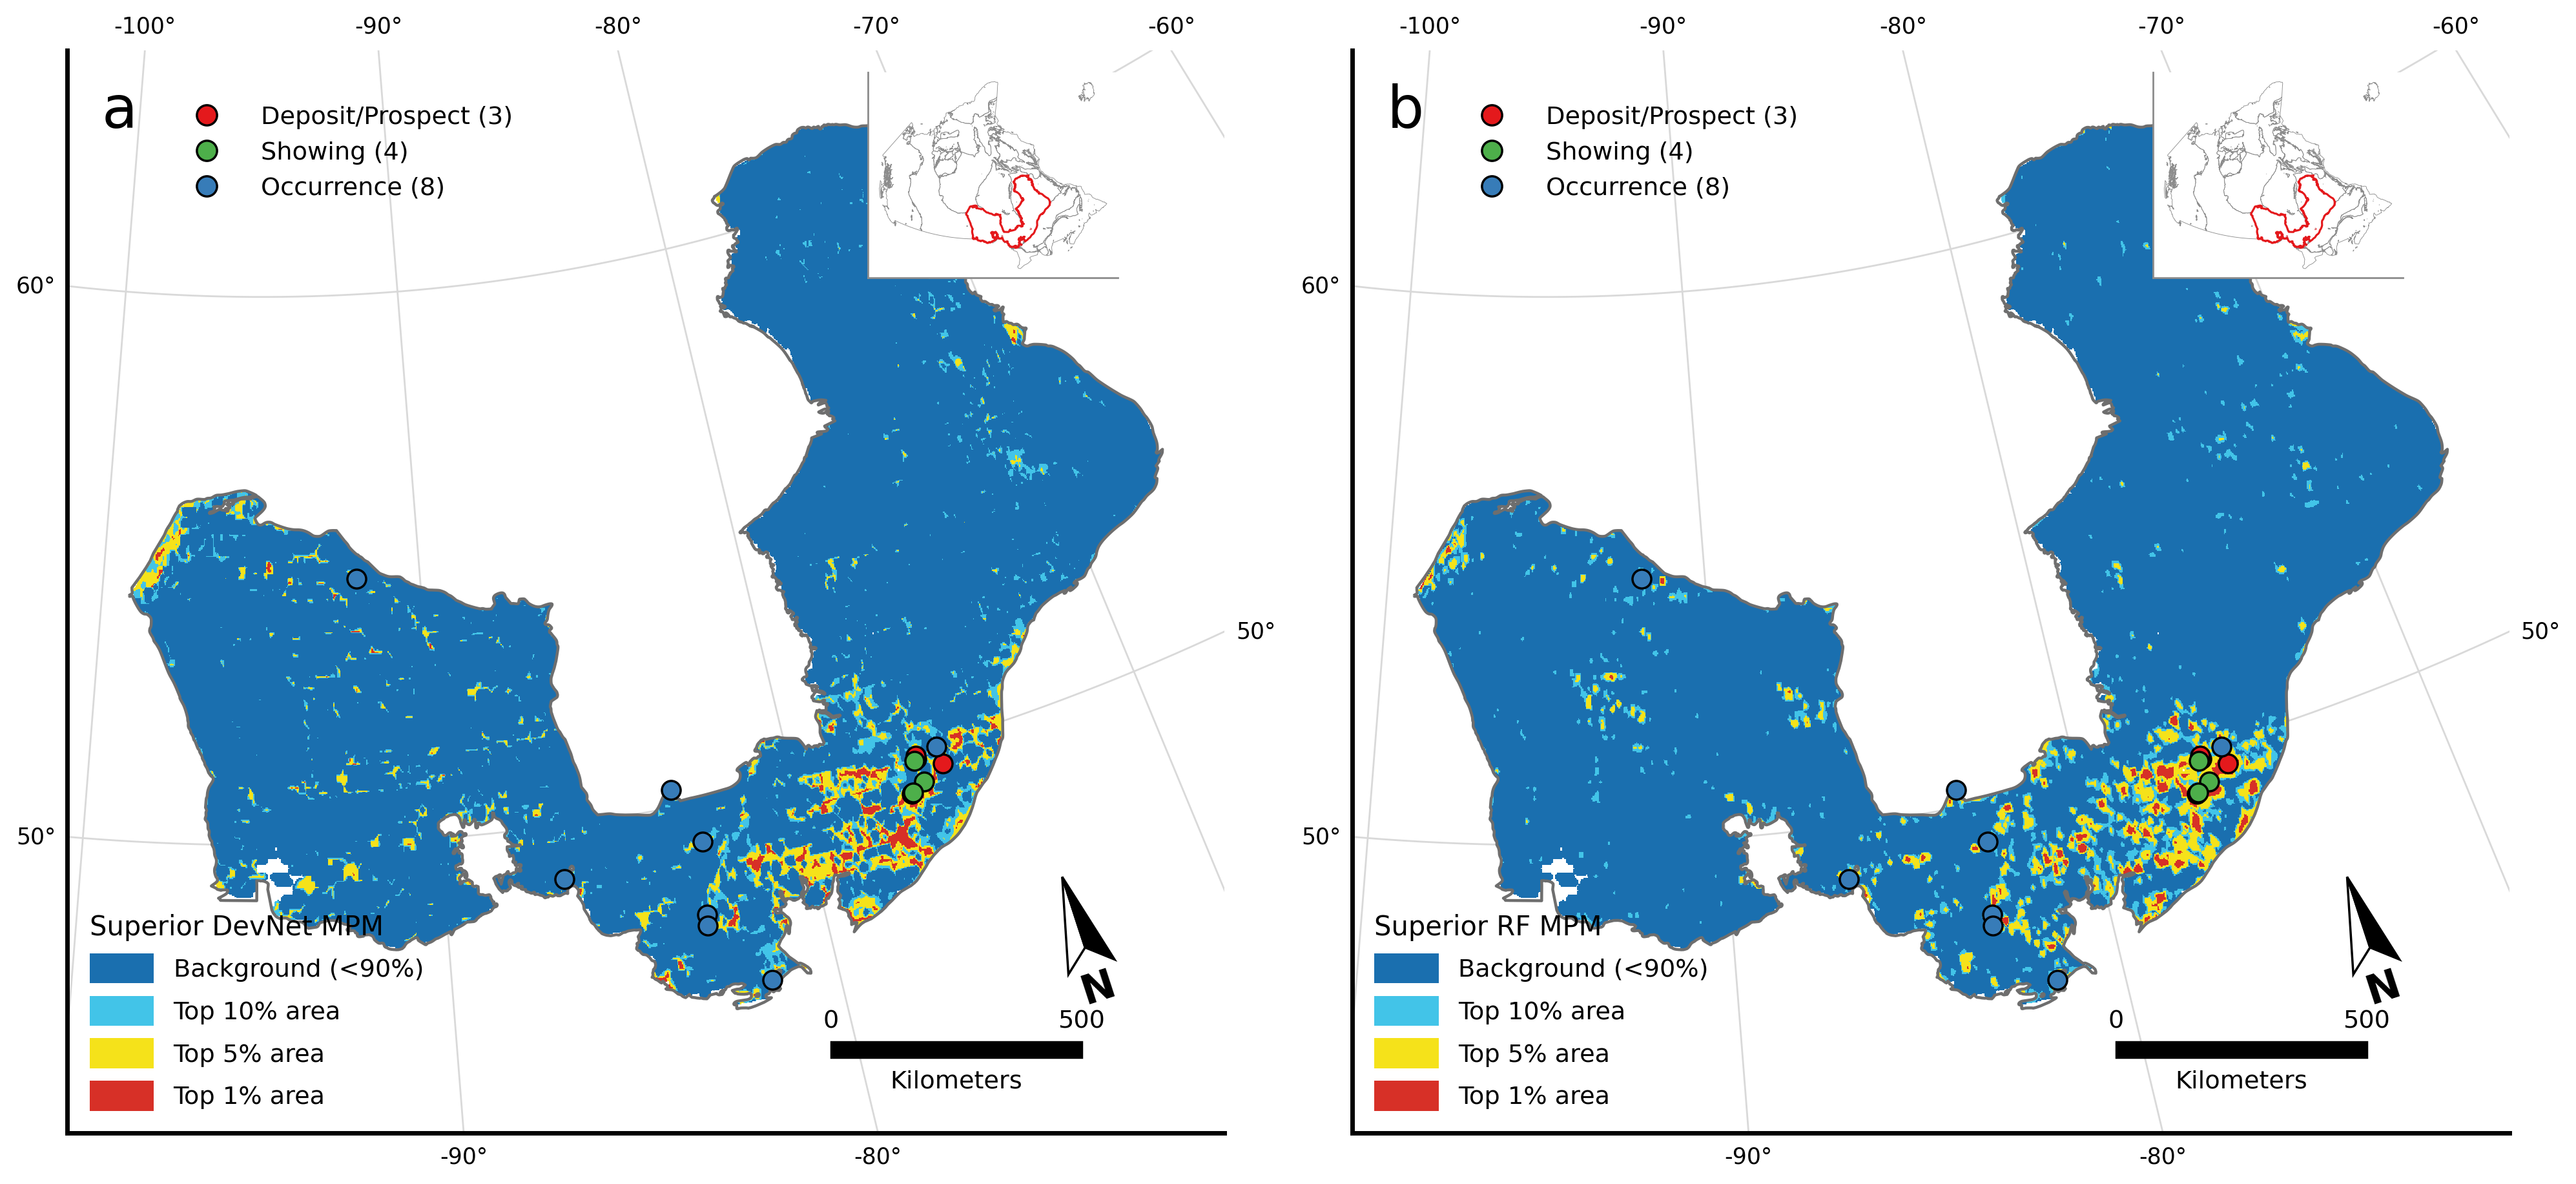
\includegraphics[width=\textwidth]{figures/fig_map_superior_r2.png}
\caption{Superior prospectivity maps from the production (a) DevNet and (b) RF models, classified by score percentile over the mapped area (top 1\%, 5\% and 10\%), with known occurrences by development class (Canada Atlas Lambert). Scores on the 0.1$^\circ$ prediction grid were interpolated to a 2~km raster.}\label{fig:maps}
\end{figure}

\begin{figure}[t]
\centering
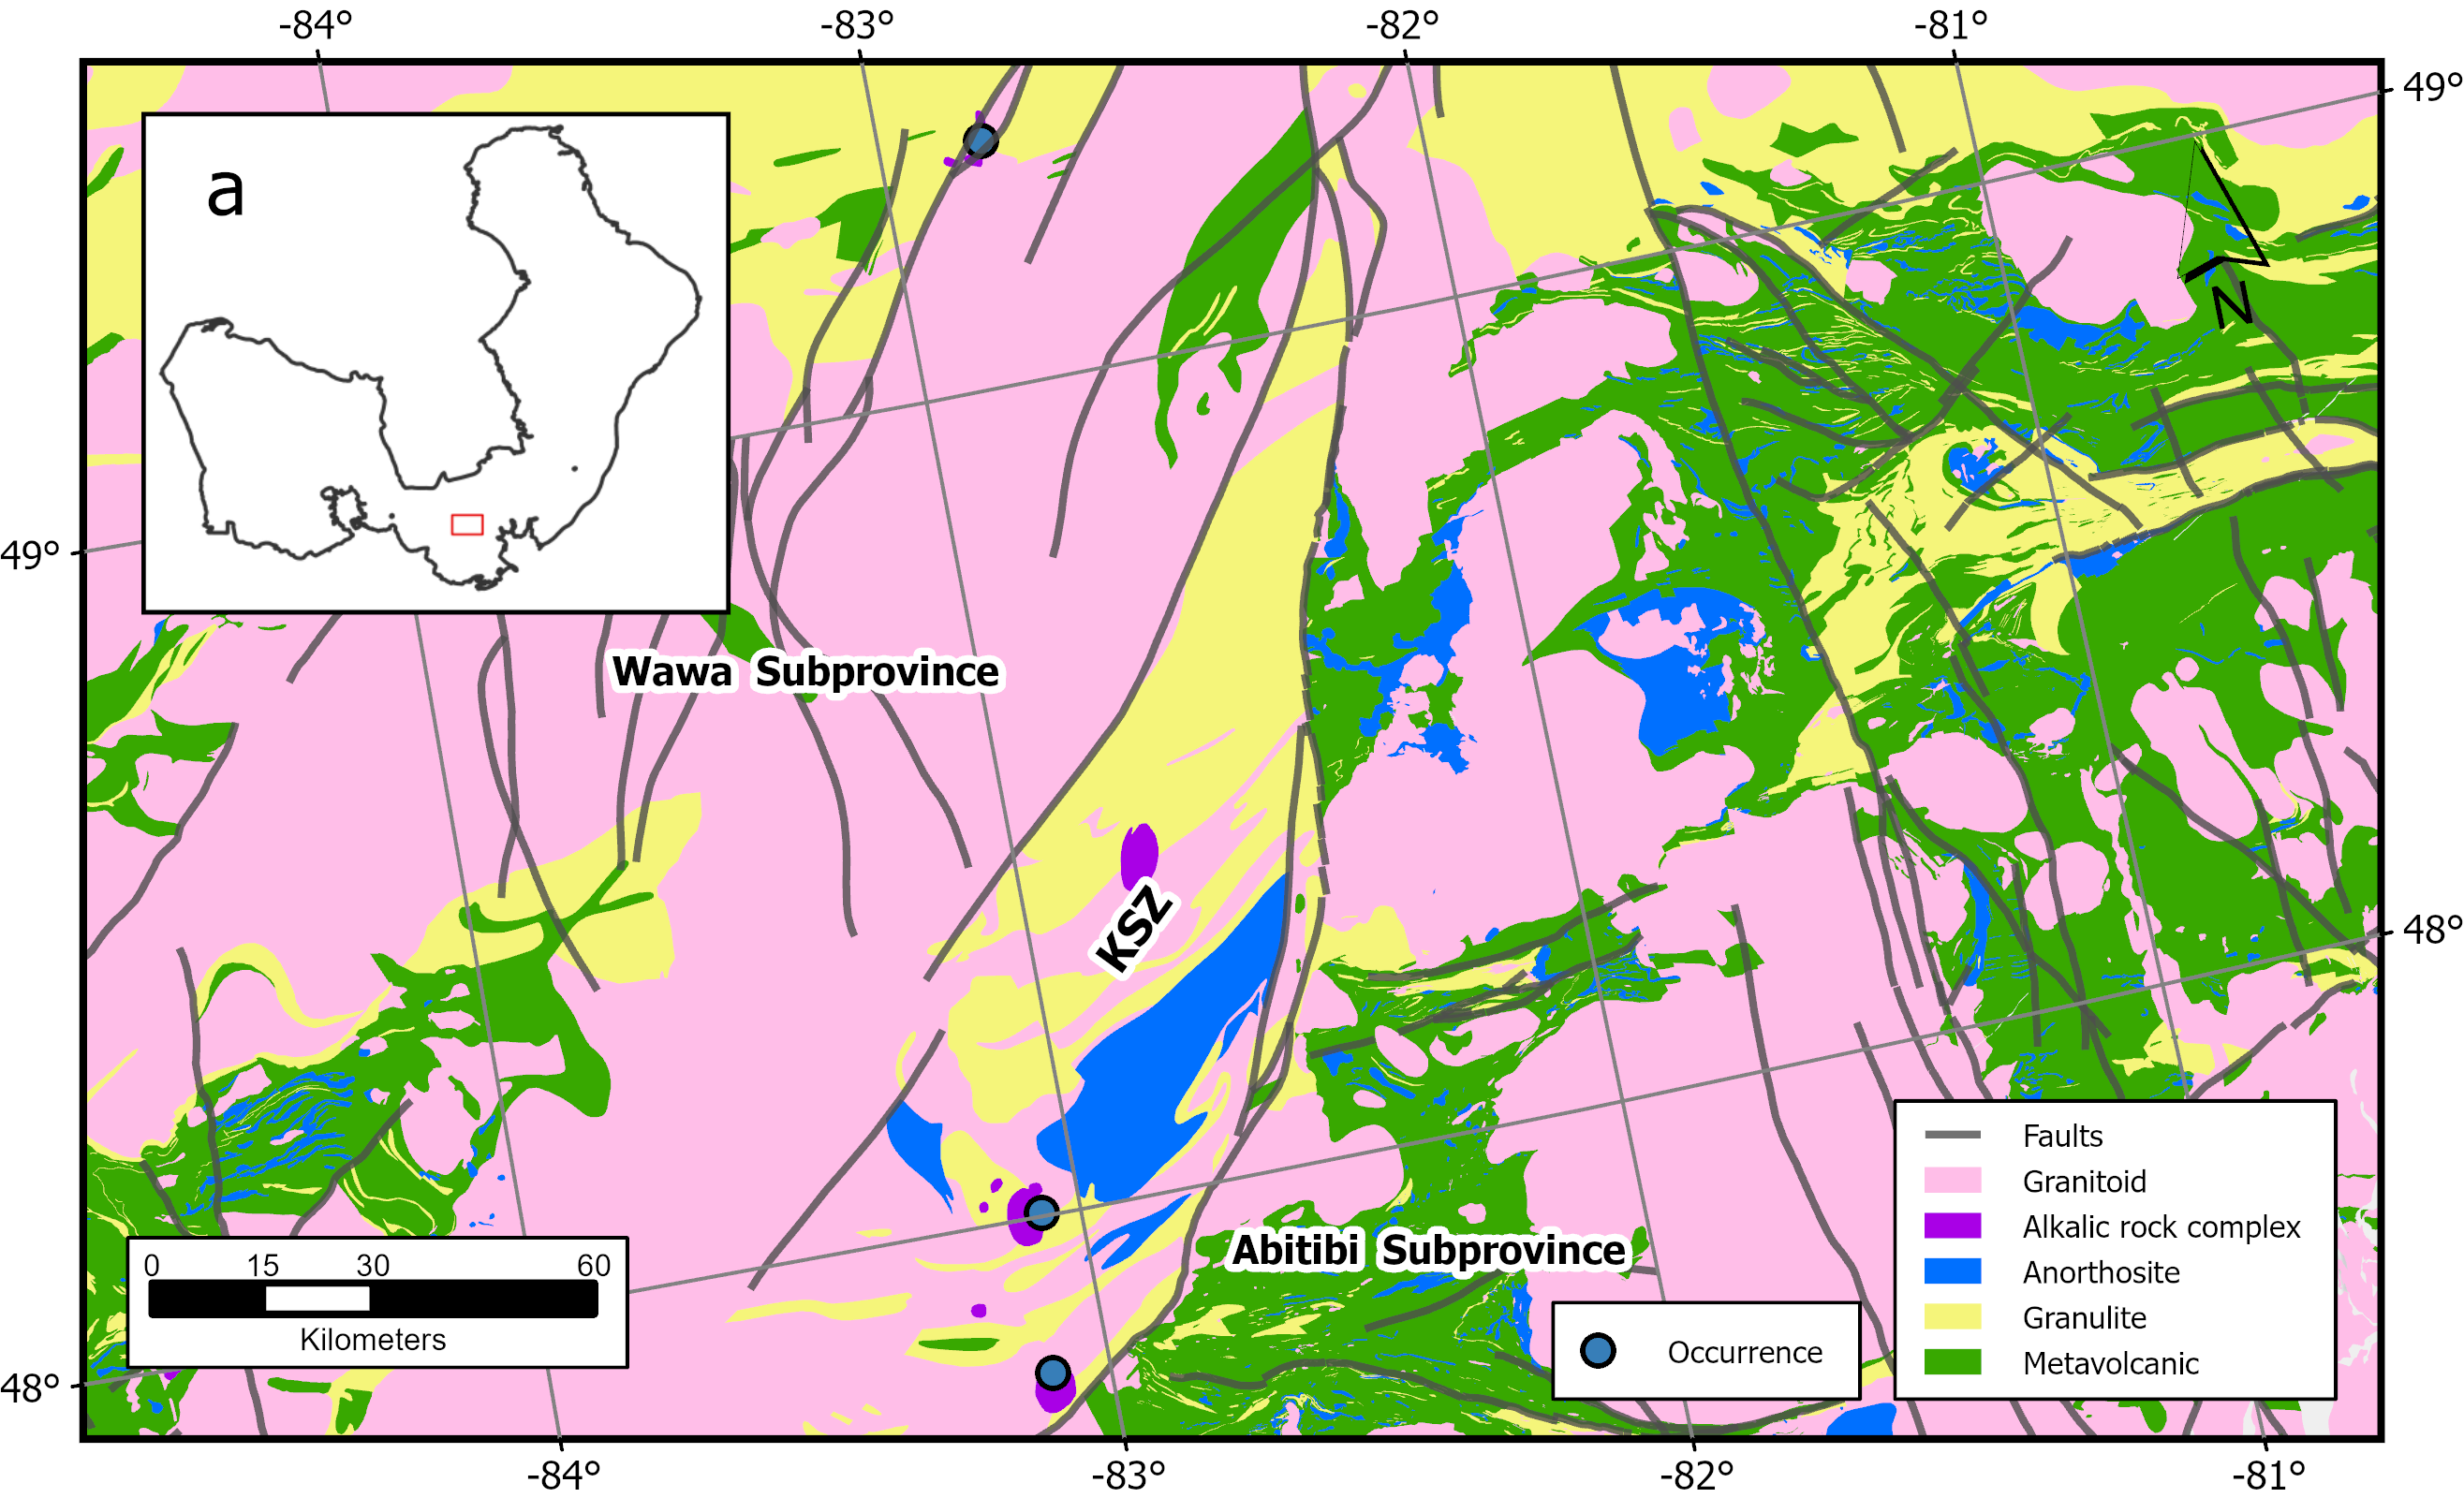
\includegraphics[width=0.49\textwidth]{figures/fig_ksz_geology.png}\hfill
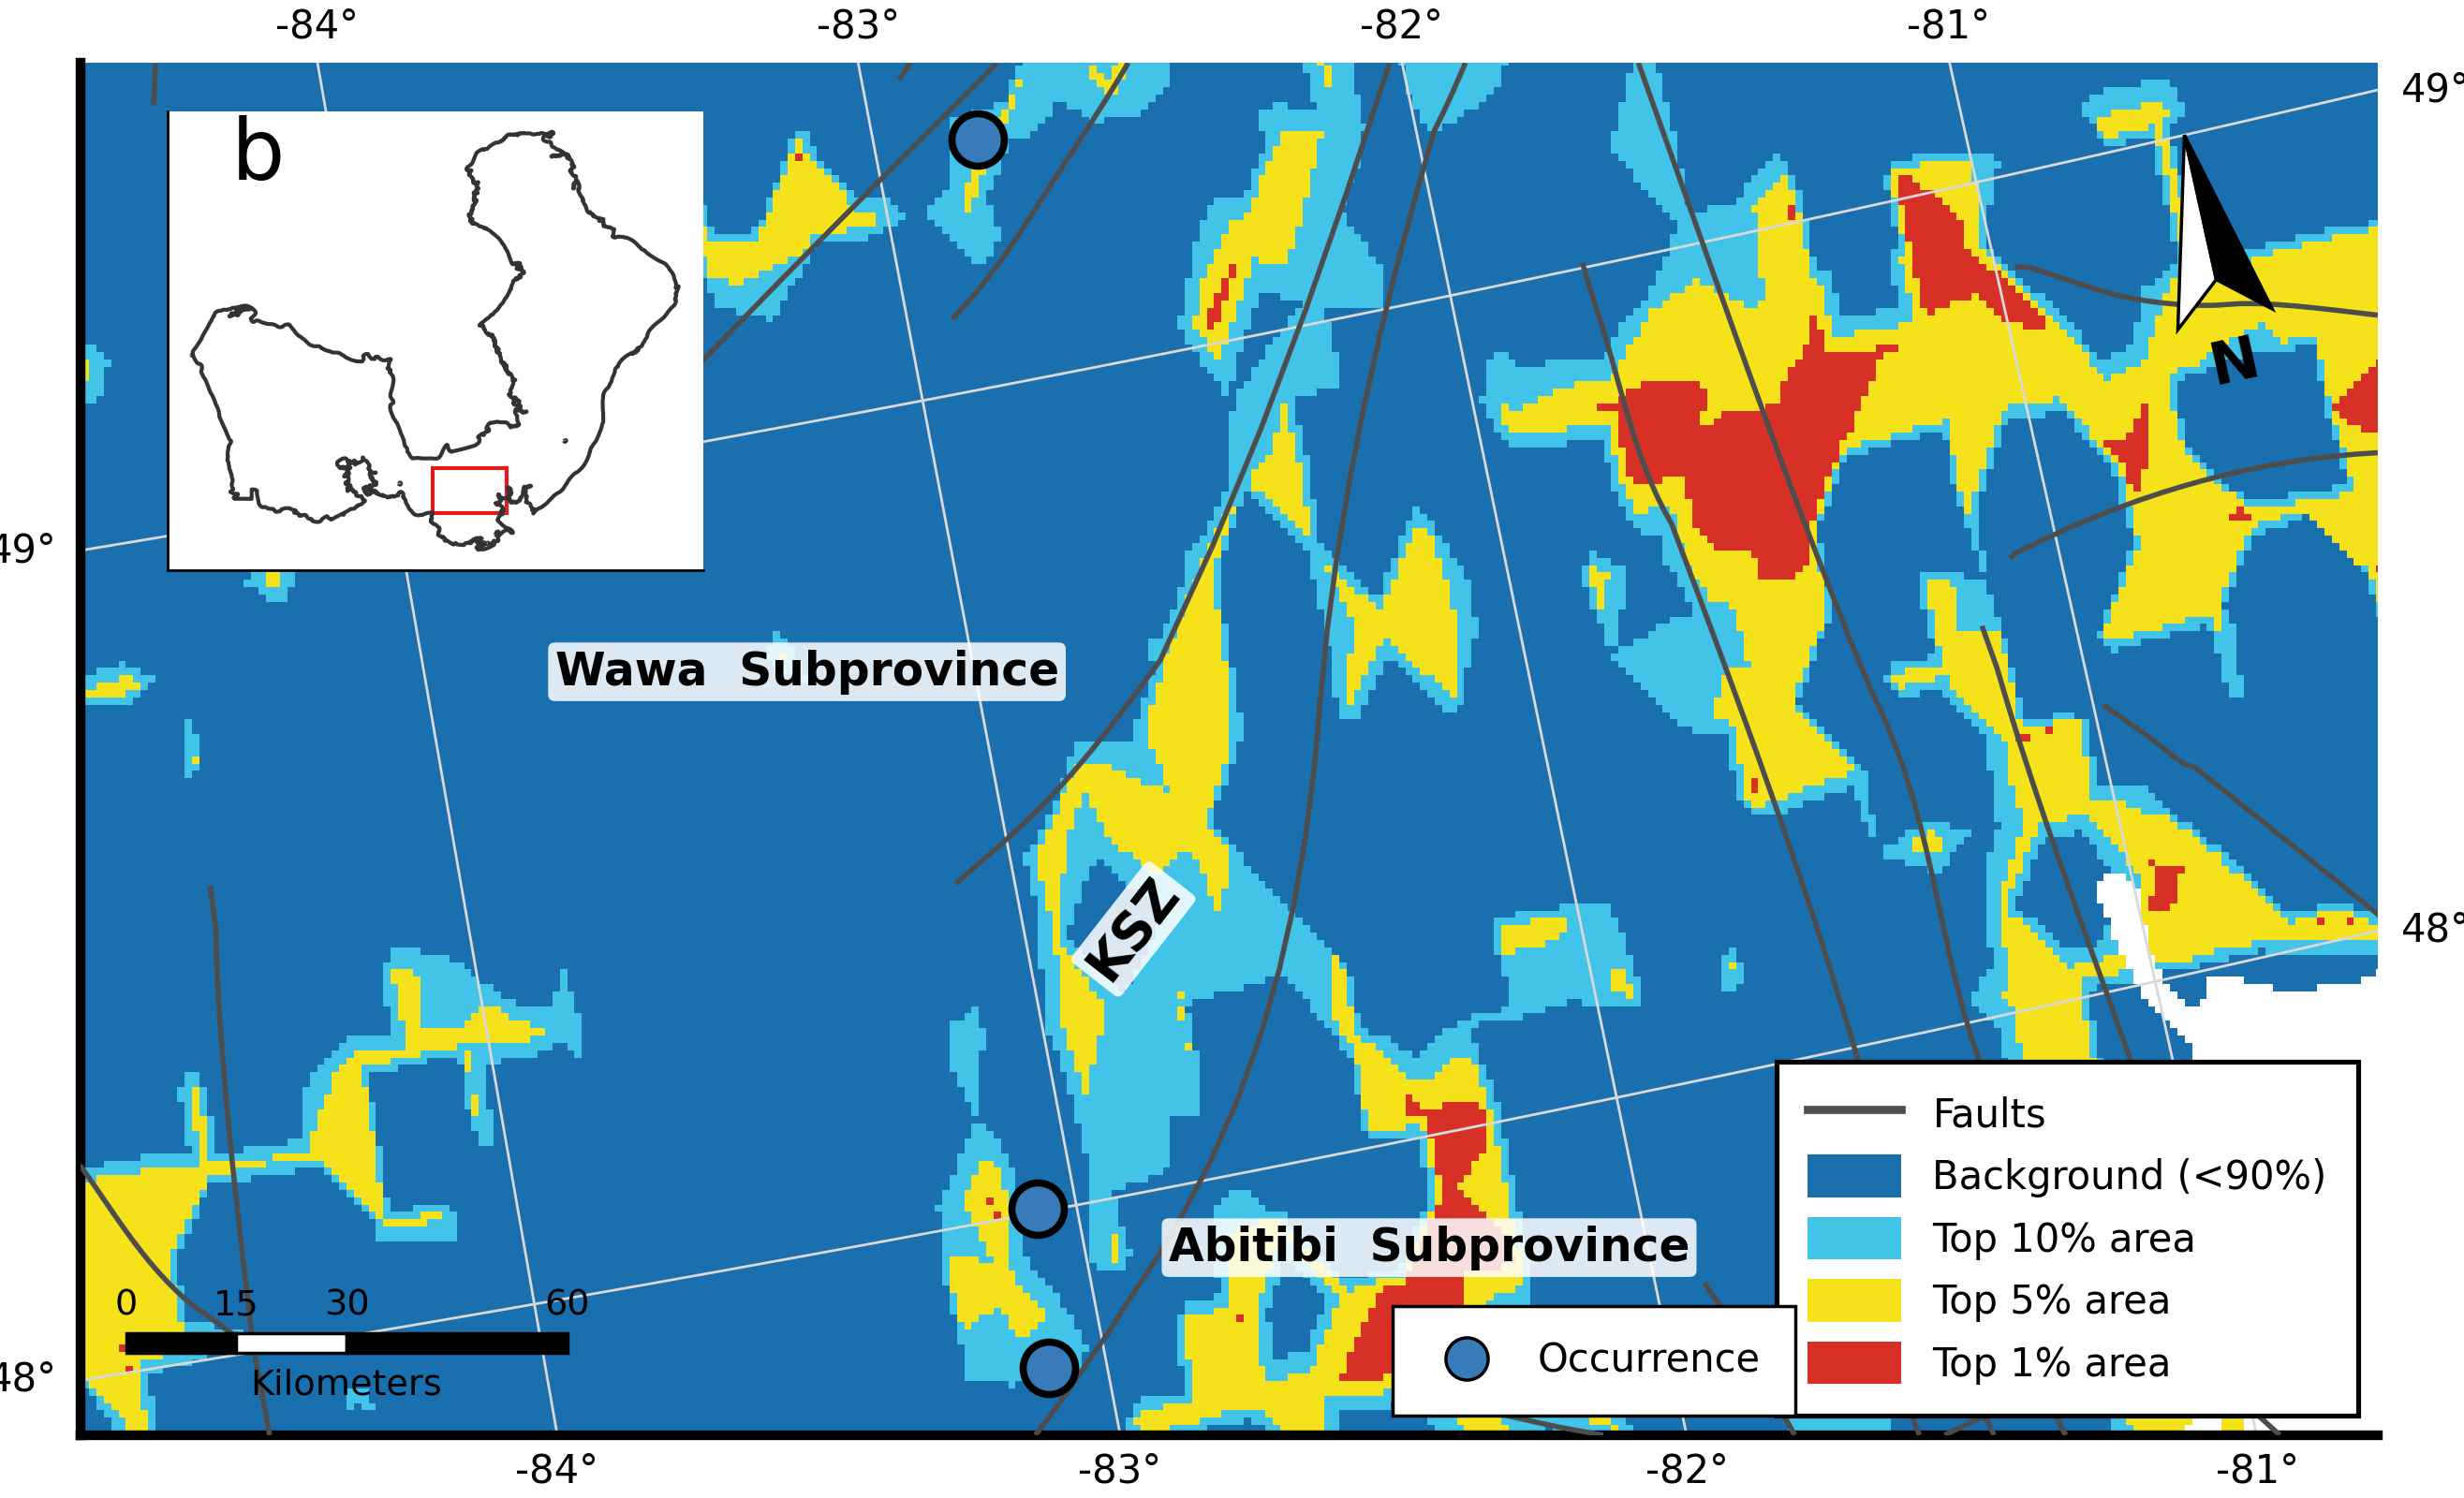
\includegraphics[width=0.49\textwidth]{figures/fig_ksz_r2.png}
\caption{Kapuskasing area. (a) Regional geology with the Kapuskasing Structural Zone (KSZ) and alkalic rock complexes \citep{Gittins1967,Percival1994}, compiled from \citet{Heather1995} and \citet{Montsion2018}. (b) DevNet top 1\%, 5\% and 10\% classes (province-wide percentiles), with faults from the compilation used as an evidence layer, on the same frame as (a).}\label{fig:ksz}
\end{figure}

The DevNet map is more stable with respect to individual occurrences than the RF map (Fig.~\ref{fig:stability}). When each of the 15 occurrences is left out in turn, 93\% of the grid nodes in the full DevNet model's top 5\% remain in the top 5\% in at least 12 of the 15 refitted models, and 1\% in fewer than half of them, whereas for RF the shares are 53\% and 28\%. RF's top classes therefore depend strongly on which occurrences are known, whereas DevNet's follow properties shared by many of them.

\begin{figure}[t]
\centering
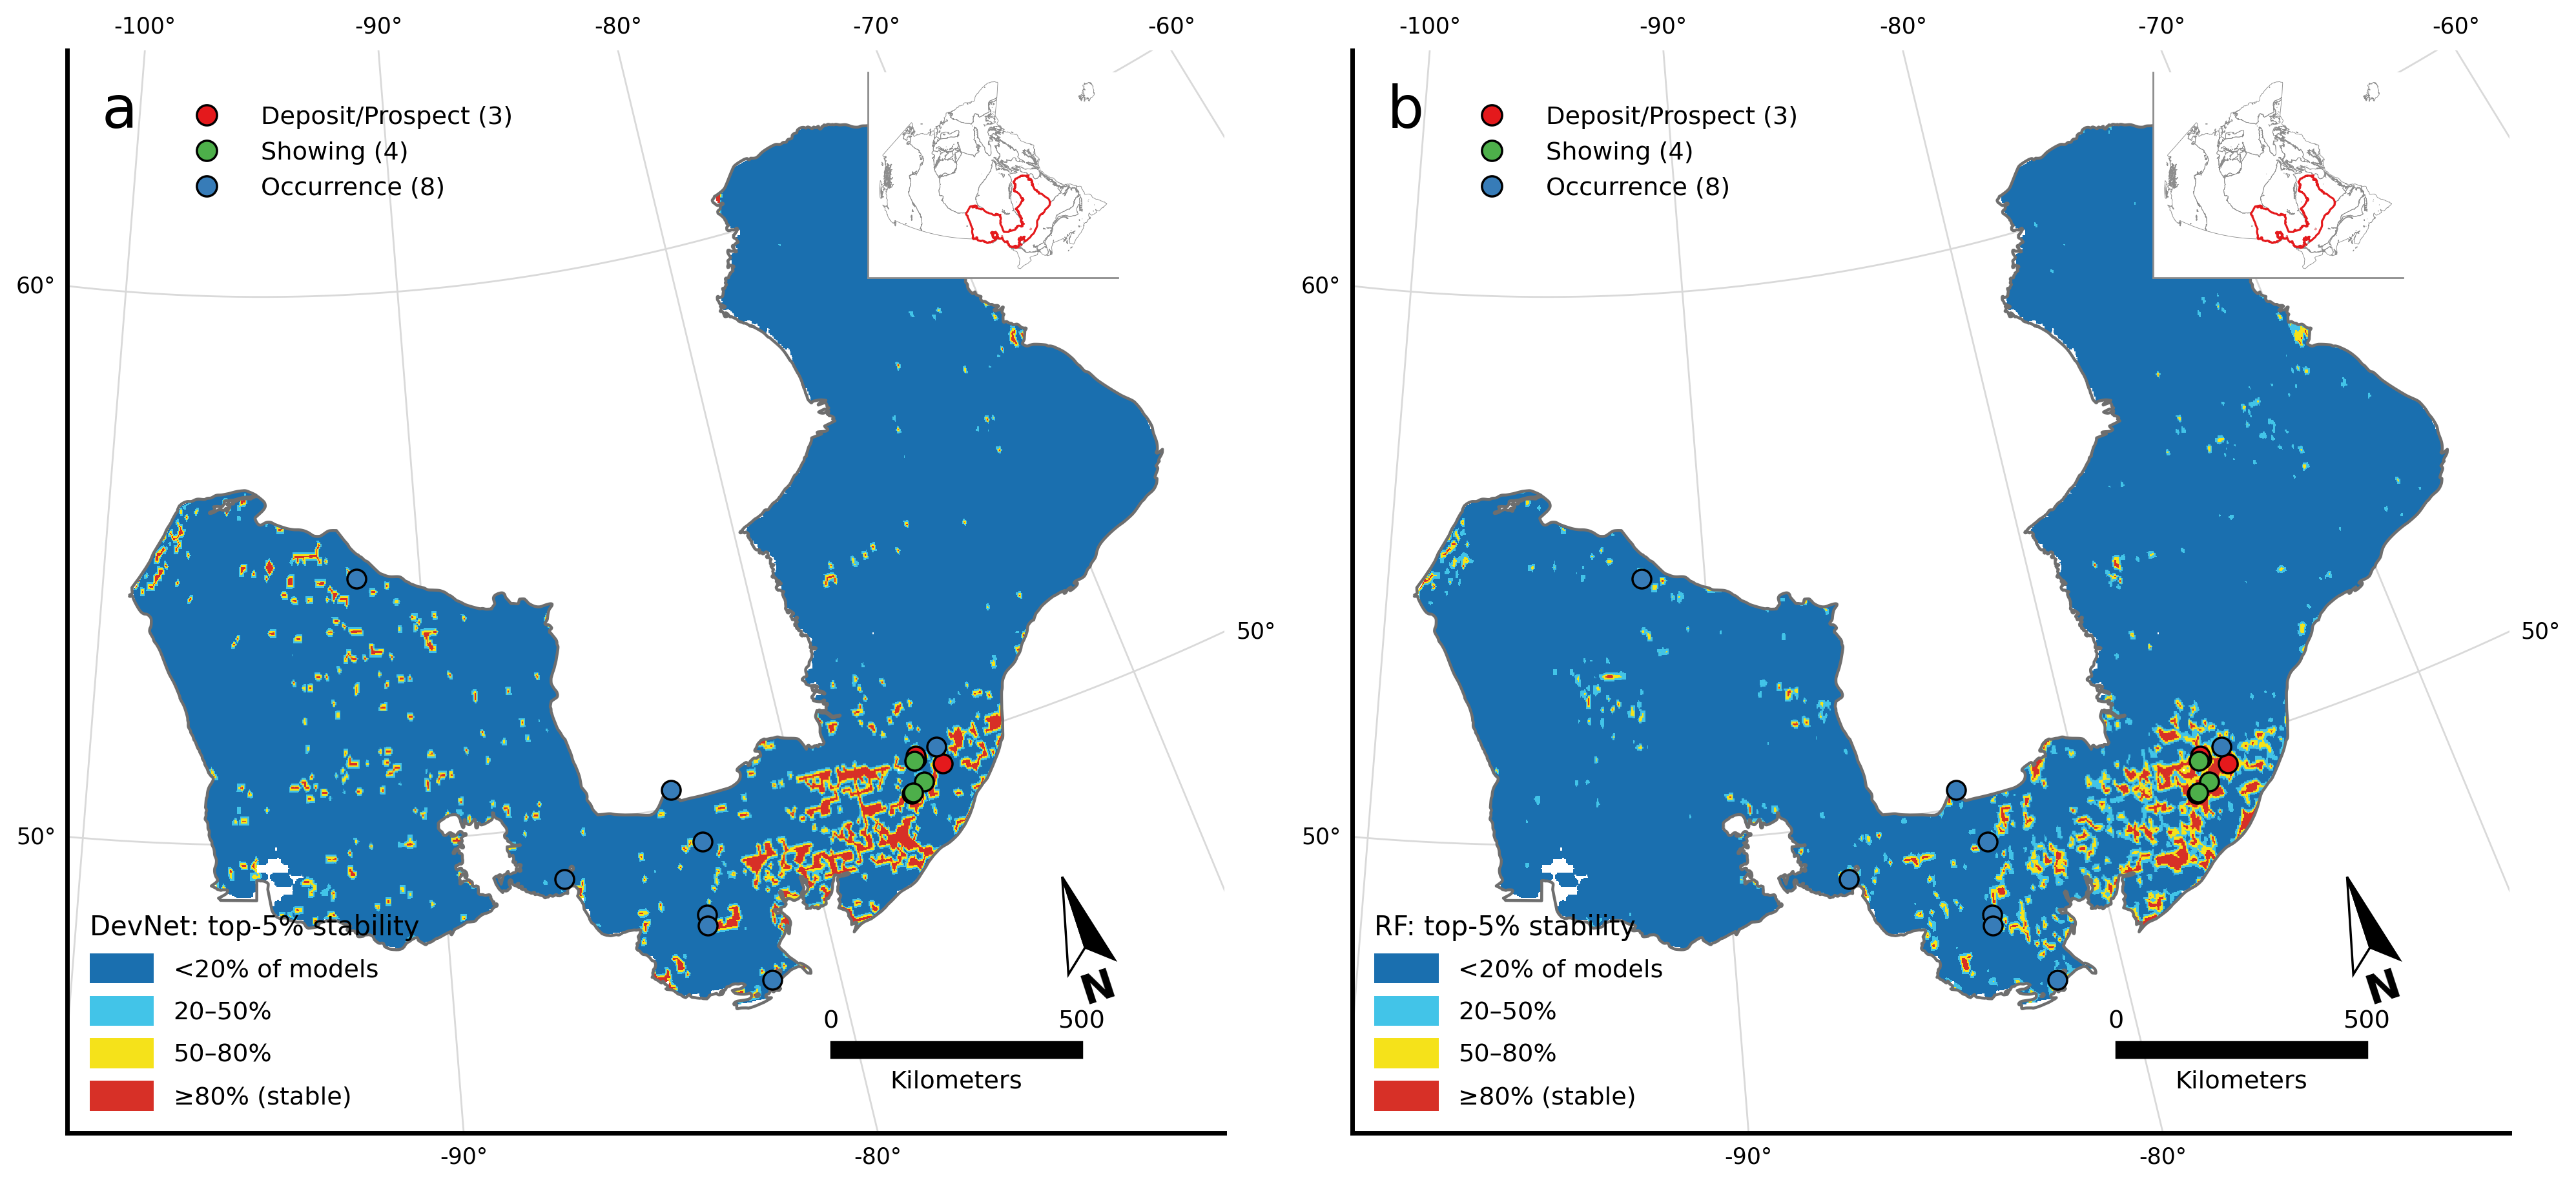
\includegraphics[width=\textwidth]{figures/fig_map_stability_r2.png}
\caption{Stability of the Superior top-5\% class with respect to individual occurrences: share of the 15 leave-one-occurrence-out models that place each 2~km cell in the province's top 5\%, for (a) DevNet and (b) RF.}\label{fig:stability}
\end{figure}

%% ===================================================================
\section{Discussion}\label{sec:discussion}

\subsection{What the semi-supervised formulation adds}\label{sec:disc-devnet}

Three results bound the answer. First, in Superior DevNet ranks held-out occurrences better than RF, tuned RF, tuned gradient boosting, bagging-PU and nnPU in every repeat of every protocol, and its lead is largest when the test requires extrapolation: RF and bagging-PU, which learn a sharp decision boundary around the training positives, lose 30--60\% of their AP once the nearest training occurrence is 50--200~km away, whereas DevNet keeps most of its AP to 100~km. With 15 positives the margin over RF is not statistically conclusive on its own, and part of DevNet's advantage reflects a design chosen with these provinces in view; but the lead is consistent across all 18 repeat--block combinations, it survives a design search for the tree-based learners, and DevNet chosen by nested selection still beats RF in 23 of 24 combinations.

Second, the ablation shows where most of this lead comes from. With all labels and the map classes, DevNet-BCE, which keeps DevNet's network, rank-normal inputs and background-heavy batches but labels the background barren, does as well as DevNet. Most of the lead over the tree-based learners therefore belongs to a smooth score over well-scaled inputs: the thresholds of tree ensembles carve out the neighbourhood of each training positive, which is rewarded when held-out occurrences lie close by and penalised when they do not. The design of the network matters within this smooth model class (Appendix~\ref{app:sensitivity}, Table~\ref{tab:ablation}). Its score is a sum of a few ReLU ridges in the space of its inputs, so its resolution along each feature is set by how that feature is scaled; on z-scored, strongly skewed layers a handful of extreme values occupy most of the input range and the bulk of the ground is compressed into a narrow interval. Quantile-normal inputs give every feature a comparable, rank-based scale, the information that trees exploit through their thresholds, while keeping the score smooth, and background-heavy batches let the loss see much more of the background per update.

Third, the tests of the semi-supervised premise show when treating the background as unlabelled rather than barren pays off: when the evidence does not mark the known complexes, and when the background contains ground that resembles the occurrences. Without point-level map classes, DevNet beats its cross-entropy twin at every label count from one training positive to all of them, and bagging-PU beats RF. With the raw map classes, where six of the 15 Superior occurrences sit on an alkalic-intrusion cell that covers 0.5\% of the background, a cross-entropy loss can exploit this near-deterministic lookup at least as well, and the two losses are level. A plausible reading is that the inlier term of the deviation loss, which pulls the scores of the whole background towards a common reference rather than pushing every background point down, regularises the score where the signal is weak and spread over many layers, whereas a supervised loss gains where one feature separates most positives from the background. Mislabelled ground around occurrences shows the premise most directly: labelling it barren cost RF almost half of its AP in Superior, whereas bagging-PU, which never treats any one background point as certainly barren, lost little, and across the three provinces the unlabelled-background member of each pair lost less in five of six comparisons and clearly more in none. A larger unlabelled pool did not favour the semi-supervised loss, contrary to our prediction.

These results matter for the use argued in Section~\ref{sec:disc-mapclasses}: finding complexes that the bedrock map does not show is the setting without map classes, and there the semi-supervised formulation helps consistently. Among formulations that treat the background as unlabelled, the deviation loss is the one that works. nnPU, which differs from DevNet only in its risk, trails it by 0.19--0.41 in AP under blocking, fails in Cordillera and Grenville and without map classes, and depends on a class prior that is unknown in practice (AP 0.13--0.26 for $\pi$ between 0.005 and 0.05); bagging-PU trails it under every protocol.

The Cordilleran and Grenville results bound the conclusion further. Where positives are comparatively plentiful and clustered (Cordillera), or the geophysical signal is weak (Grenville), the tree-based learners are as good or better under random splits, a coordinate-only forest matches them, and no model transfers between blocks. DevNet is therefore not a universal replacement for discriminative baselines; its advantage is specific to the combination of very few positives, a shared control and the need to extrapolate.

\subsection{Geological map classes: evidence and lookup}\label{sec:disc-mapclasses}

The map classes move every model more than the choice of model does. Withholding them costs DevNet and RF about half or more of their AP, and a single class, alkalic intrusive rock, carries over a third of DevNet's blocked AP. Six of the 15 Superior occurrences lie on cells mapped as alkalic intrusive rock, which covers 0.5\% of the background; for these occurrences the map already marks the target. The age-contact flag of the containing cell partly does the same, because a Proterozoic complex mapped within Archean crust creates an age contact, and DevNet ranks it second.

Whether such lookup is acceptable depends on the use. For targeting within mapped complexes, or for ranking known complexes by their geophysical setting, a mapped alkaline intrusion is legitimate and strong evidence, and the full inputs are appropriate. For finding complexes that the 1:5,000,000 map does not show, it is not, and the relevant skill is that without map classes: an AP of 0.08--0.13 under spatial blocking, 16--27 times the random-ranking value but well below what the full inputs suggest. Comparisons between studies, and claims about how well a model ``discovers'' occurrences, should state which of the two is being measured. In both settings DevNet is at or near the top under blocking, and without map classes its semi-supervised loss itself adds skill (Section~\ref{sec:res-ablation}); its absolute skill, however, depends strongly on the map classes.

\subsection{Why the provinces differ}\label{sec:disc-provinces}

Grenville is the weakest of the three provinces for every model and Superior the strongest. The evidence layers are the same national compilations everywhere and almost complete (about 0.01\% of values missing in each province), so the contrast does not reflect data coverage. It follows instead from the label sets and from the geology they sample (Table~\ref{tab:region-diag}).

First, the effective number of independent occurrences is smaller than the count suggests, and smallest in Grenville. Merging occurrences within 10~km leaves 12 sites of 15 occurrences in Superior, 17 of 27 in Cordillera and 8 of 12 in Grenville, and in Cordillera and Grenville more than half of the occurrences share a site with another (median distance to the nearest other occurrence 7~km, against 31~km in Superior). Under a random split such neighbours fall on both sides, which is why coordinates alone score well in these two provinces (Section~\ref{sec:res-geography}) and why their skill collapses under blocking.

Second, only in Superior do distant occurrences share a geophysical signature. There the far-neighbour index has a median of 0.005, an order of magnitude below that of random pseudo-occurrences (0.049; 5th percentile 0.022): an occurrence resembles another occurrence more than 100~km away more closely than it resembles all but a few background points. In Cordillera (0.032 against 0.027) and Grenville (0.046 against 0.066) the index falls within the range of the random sets, so there is no shared signature for a model to transfer. The univariate evidence agrees: the median feature separates occurrences from background with $|\mathrm{AUC}-0.5| = 0.15$ in Superior but only 0.05 and 0.06 in Cordillera and Grenville, where three features and one feature respectively exceed 0.25.

Third, the Grenville label set mixes carbonatites of different ages and tectonic settings. Crevier is a late-Grenvillian alkaline--carbonatite intrusion of about 957~Ma \citep{Groulier2020}. St-Honoré, with Terres Rompues on the same complex, was emplaced at about 580~Ma in the Saguenay graben of the St.~Lawrence rift system \citep{Neron2018}. The Lavergne--Springer occurrences lie near Lake Nipissing at the western end of the Ottawa--Bonnech\`ere graben, and the Cantley, Quinnville and Templeton showings near Gatineau belong to the calcite-rich veins and dykes of the Grenville marble belts, whose magmatic origin has long been debated \citep{Moecher1997}. The far-neighbour index tracks this heterogeneity. The rift-related St-Honoré, Terres Rompues and Lavergne--Springer occurrences, about 700~km apart, resemble one another closely (indices 0.005--0.033), whereas Crevier (0.19), Megiscane Lake (0.28) and Sullivan Island (0.15) resemble no other occurrence. Age diversity alone is not the problem, since the Superior occurrences also span several magmatic episodes \citep{Rukhlov2010}. They were, however, all emplaced into the same stable cratonic lithosphere, whose margins and crustal-scale structures the present-day LAB, Moho and potential-field layers still record. The Grenville crust was reworked by the Grenvillian orogeny and by later rifting, so its present-day geophysics need not record a common setting for occurrences that formed in different ones. The mapped geology adds noise of its own: the twelve Grenville occurrences fall on Archean, Proterozoic and Paleozoic map units, because the bedrock map records reworked protoliths and the Paleozoic cover over St-Honoré rather than the carbonatites, and none of them lies on a cell mapped as alkalic intrusive rock, whereas about 5\% of the Grenville background does.

Missing or coarse geophysics therefore explains little of the contrast; the number, independence and geological coherence of the labels explain most of it. A model for Grenville would need either more occurrences of one carbonatite type or separate models for rift-related and orogenic types, which the present label set cannot support.

\begin{table}[t]
\caption{Province diagnostics. Sites: occurrences merged by single linkage at 10~km; shared: share of occurrences that share a site; NN: median distance to the nearest other occurrence; eras: number of geological-era classes mapped at the occurrences. $|\mathrm{AUC}-0.5|$: median over features (occurrences against the evaluation background) and number of features with $|\mathrm{AUC}-0.5| \geq 0.25$. Far-neighbour index: median over occurrences, geophysical and structural layers; random: median [5th percentile] of the same statistic for 200 random sets of background points.}\label{tab:region-diag}
\scriptsize
\setlength{\tabcolsep}{2.5pt}
\begin{tabular*}{\textwidth}{@{\extracolsep\fill}lccccccccc}
\toprule
 & \multicolumn{5}{c}{Label set} & \multicolumn{2}{c}{$|\mathrm{AUC}-0.5|$} & \multicolumn{2}{c}{Far-neighbour index} \\
\cmidrule(lr){2-6}\cmidrule(lr){7-8}\cmidrule(lr){9-10}
Region & Occ. & Sites & Shared & NN (km) & Eras & Median & $\geq 0.25$ & Occurrences & Random \\
\midrule
Superior & 15 & 12 & 33\% & 31 & 2 & 0.15 & 6 & 0.005 & 0.049 [0.022] \\
Cordillera & 27 & 17 & 56\% & 7 & 2 & 0.05 & 3 & 0.032 & 0.027 [0.015] \\
Grenville & 12 & 8 & 58\% & 7 & 3 & 0.06 & 1 & 0.046 & 0.066 [0.031] \\
\botrule
\end{tabular*}
\end{table}

\subsection{Synthetic positives do not create information}\label{sec:disc-gan}

Synthetic positives are an attractive response to label scarcity, and GAN-generated labels have been recommended for exactly this commodity \citep{Parsa2025}. Our results counsel caution. A generator fitted to a dozen training positives has two options. It can stay close to them, in which case it adds near-duplicates that carry no new information (jitter and SMOTE, nearest-neighbour ratios of 0.1--0.2); or it can spread out, in which case it must guess where unseen occurrences lie and, having no information about that, places part of its mass in background-like feature space (WGAN-GP, 35\% of samples nearest to a background point). Neither option supplies the information that is actually missing, namely what undiscovered occurrences look like. The gains for RF from jitter are better explained as smoothing: synthetic points around the training positives make more trees vote for nearby held-out points, which relieves RF's degenerate surface of exactly-zero probabilities rather than teaching it new geology. Consistent with this reading, they vanish and turn into losses with 200~km blocks, where held-out occurrences are far from every training one, and DevNet, whose loss already produces smooth scores, gains nothing from the same points. Where synthetic positives are used, they must be generated inside each training fold from that fold's positives only, and performance must be measured on real held-out occurrences; otherwise a synthetic copy of a training occurrence in the test set reproduces the sibling problem of Section~\ref{sec:res-audit} in another form.

\subsection{The validation protocol decides many reported differences}\label{sec:disc-protocol}

Four of our findings concern evaluation rather than models. First, with tens of positives a single cross-validation split gives a noisy estimate: re-splitting the same Superior data moves each model's AP over a range of 0.07--0.17 (Table~\ref{tab:benchmark}), as large as many of the differences between models. Second, random splits overstate skill wherever occurrences cluster, and the size of the overstatement differs between models, so random splits can also reverse a model ranking (Section~\ref{sec:res-spatial}). Third, splitting augmented child cells at random yields near-perfect test AUC on these data whatever the negatives, because almost every test positive has a sibling, sharing the coarse deep-architecture values and the map classes exactly and the fine-scale values nearly, on the training side. In this design the held-out test asks the model to recognise a location it has already seen, and the comparison of training and test AUC, which \citet{Parsa2024} used to argue that their models were not over-fitted, becomes uninformative because the test set is not independent of the training set. Selecting negatives from the least similar 5\% of the ground adds a second, independent source of optimism: it removes from evaluation exactly the ground on which a prospectivity model is hardest to get right. Fourth, the geological map classes can supply a large share of the reported skill by marking known complexes (Section~\ref{sec:disc-mapclasses}), which no split design removes.

We stress what the audit does and does not show. It uses our inputs, regions and models, not those of \citet{Parsa2024}, and it does not establish what their numbers would have been under a grouped split. It does show that, on comparable Canadian carbonatite data, the published design produces test AUCs close to 1 whether the underlying skill is high (Superior) or modest (Grenville, honest AUC 0.77), and that the reported 0.91--0.96 cannot be taken as evidence of generalisation to unexplored ground until the augmented children of one occurrence are kept on one side of the split. \citet{Parsa2025} describe the same stratified random 70/30 split for a workflow that adds GAN-generated labels; their description does not state whether synthetic labels derived from an original label were kept on the same side of the split as that label. If they were not, the caveat applies with greater force. For prospectivity studies under extreme label scarcity we therefore recommend (i) grouping every augmented or near-duplicate label with its source occurrence before any split, (ii) drawing evaluation negatives at random from the domain rather than from the ground least similar to the positives, (iii) reporting AP with intervals over repeated splits rather than a single AUC, (iv) adding a spatially blocked validation in which training background is purged from held-out blocks, (v) reporting a geography-only baseline, so that readers can see how much of a score is location, and (vi) reporting results with and without point-level map classes, so that readers can see how much of a score is map lookup.

\subsection{Geological interpretation}\label{sec:disc-geology}

The drivers on which RF and DevNet agree in Superior describe a coherent setting. Shallower LAB, together with the strong ranking of deep-source magnetic gradients, points to the thinner lithosphere at the edges of the thick Superior root, where small-degree melting of metasomatised mantle and access along lithosphere-scale structures are most likely \citep{Griffin2013,Groves2021,Hoggard2020}; a mantle conductor beneath the southern Abitibi is consistent with such metasomatism \citep{Snyder2021}. Fault proximity and high magnetic intensity capture the structures that focus ascent and the magnetite-bearing intrusions themselves \citep{Thomas2016}. The negative effect of proximity to deep magnetic worms is less intuitive; it may reflect the concentration of deep magnetic contacts along terrane boundaries that are not themselves carbonatite hosts, and should not be over-interpreted.

The strong positive effect of greenstone lithology and of proximity to regional greenstone units needs more care. Eight of the 15 occurrences belong to the eastern-Abitibi cluster in a greenstone-dominated subprovince, so the association may partly record where the largest cluster lies rather than a control shared by the dispersed occurrences; the dispersed occurrences that DevNet ranks lowest under blocking, Kapuskasing and Nemegosenda Lake, lie in the high-grade and alkaline terrain of the KSZ rather than in a greenstone belt. Consistent with this, DevNet's map follows the KSZ only in discontinuous patches, while the untrained Clay-Howells resource on the KSZ still ranks at its 97th percentile. A model whose top classes are tied to one greenstone-hosted cluster is useful for ranking ground of that type, but it should not be expected to recognise alkaline complexes in other settings as well.

\subsection{Limitations}\label{sec:limitations}

Fifteen positives allow only weak statistical statements: our firm results are those that are consistent across repeats, block sizes, comparisons and provinces. DevNet's input representation and batch composition were chosen with diagnostic experiments on these three provinces, and the nested selection shows that part of the final configuration's advantage reflects that choice; confirmation on an independent province is needed, and the Churchill Province, the obvious candidate, holds too few carbonatite-hosted occurrences after deduplication for a meaningful test. The geological encoding used here replaced a coarser grouping of lithologies after that grouping had been evaluated; the change raised the AP of every model except nnPU under random splits and 50--100~km blocks but not with 200~km blocks. The evaluation background may contain undiscovered occurrences, so all metrics are lower bounds. The test with background added near occurrences is a stress test: 20--50 points per occurrence far exceed the density of the training background, which places about one point in each 2--10~km annulus, so it shows sensitivity to mislabelled ground rather than its size in practice. Radiometric data could not be used because of incomplete coverage, and whole-rock geochemistry is too sparse to serve as an input. Eleven gravity and magnetic layers are proprietary Getech products; equivalent derivatives can be computed from the public parent grids, but results will differ somewhat. The provenance of the fault compilation should be confirmed against the original data release before publication. The occurrence-class information (Deposit/Prospect, Showing, Occurrence) was not used for weighting; with 3--8 occurrences per class, confidence-weighted training could not be evaluated reliably. Finally, maps are per-region percentiles and are not calibrated probabilities.

%% ===================================================================
\section{Conclusions}\label{sec:conclusions}

For regional carbonatite-hosted REE prospectivity mapping with 12--27 occurrences per province:
\begin{enumerate}
\item In the Superior Province a semi-supervised Deviation Network ranks held-out occurrences better than Random Forest, tuned Random Forest and gradient boosting, bagging-PU and nnPU in every repeat under random and 50--200~km spatially blocked cross-validation (AP 0.45 and 0.42--0.25 against 0.27 and 0.19--0.15 for RF); with 15 occurrences the margin over RF is consistent but not statistically conclusive.
\item DevNet's lead over the tree-based learners comes mainly from a smooth score over rank-normal inputs with background-heavy batches: with the full inputs, an ablation that labels the background barren (cross-entropy) does as well. Treating the background as unlabelled pays off when the evidence does not mark the known complexes: without point-level map classes DevNet beats its cross-entropy twin at every label count (15--20 of 20 repeats) and bagging-PU beats RF, and labelling ground around occurrences barren almost halves RF's AP but barely affects bagging-PU, a pattern that recurs in all three provinces. Among unlabelled-background formulations the deviation loss clearly outperforms nnPU and bagging-PU.
\item Geological map classes move every model more than the choice of model. A single mapped alkalic-intrusion class, covering 6 of 15 Superior occurrences and 0.5\% of the background, carries over a third of DevNet's blocked AP, and without point-level map classes DevNet and RF lose about half or more of their skill. Prospectivity studies should report results with and without such classes.
\item In the Cordilleran Orogen and the Grenville Province the tree-based learners lead under random splits, a forest given only coordinates matches them, and no model transfers between blocks; the number, independence and geological coherence of the labels, not data coverage, explain the contrast.
\item Synthetic positives from jitter, SMOTE or a tabular WGAN-GP, generated strictly within training folds, gave DevNet no gain and RF only gains that vanish at 200~km; splitting augmented child cells of one occurrence between training and test sets yields near-perfect test AUC irrespective of skill.
\item RF and DevNet agree on the direction of all 30 leading drivers across the three provinces. DevNet's Superior map is more stable than RF's when occurrences are left out, places the untrained Clay-Howells Fe--REE--Nb resource at its 97th percentile, and favours greenstone-hosted settings like the dominant Abitibi cluster.
\end{enumerate}

\backmatter

\bmhead{Acknowledgements}
This work began as an MSc Independent Research Project at Imperial College London. We thank Ross Smail (Getech Group plc), Prof. Chetan Nathwani and Prof. Rebecca Bell for supervision, Getech Group plc for providing processed gravity and magnetic grids, and Junlin Fang for discussions on methodology and model evaluation.

\section*{Declarations}

\bmhead{Funding} %% TODO(author)
Not applicable.

\bmhead{Competing interests} %% TODO(author)
The authors declare no competing interests.

\bmhead{Data availability}
Occurrence labels are derived from \citet{Orris2018} and \citet{Parsa2024}; the deduplicated tables and study-area outlines are distributed with the code. Public layers are available from \citet{McCafferty2023}, \citet{Jobin2017}, \citet{Miles2016}, \citet{BradleyDC2008} and \citet{Wheeler1996}. Eleven processed gravity and magnetic grids were supplied by Getech Group plc under licence and cannot be redistributed.

\bmhead{Code availability} %% TODO(author): make the repository public or archive it (e.g. Zenodo) before submission
The pipeline, every analysis in this paper and the scripts that generate its tables and figures are available at \url{https://github.com/miaozhou-312/ree-prospectivity-paper}.

\begin{appendices}

\section{Additional results}\label{app:full}

\begin{table}[!h]
\caption{AUC (median over six repeats) for the runs of Table~\ref{tab:spatial}. Bold: highest AUC in each row.}\label{tab:spatial-auc}
\footnotesize
\setlength{\tabcolsep}{3pt}
\begin{tabular*}{\textwidth}{@{\extracolsep\fill}llcccc}
\toprule
Region & Split & DevNet & RF & Bagging-PU & nnPU \\
\midrule
\multirow{4}{*}{Superior} & random & 0.972 & \textbf{0.983} & 0.976 & 0.838 \\
 & 50 km & \textbf{0.973} & 0.963 & 0.965 & 0.824 \\
 & 100 km & \textbf{0.950} & 0.904 & 0.945 & 0.832 \\
 & 200 km & 0.783 & \textbf{0.880} & 0.855 & 0.814 \\
\midrule
\multirow{4}{*}{Cordillera} & random & 0.914 & 0.931 & \textbf{0.936} & 0.553 \\
 & 50 km & 0.863 & 0.849 & \textbf{0.866} & 0.545 \\
 & 100 km & 0.790 & 0.776 & \textbf{0.847} & 0.541 \\
 & 200 km & \textbf{0.821} & 0.740 & 0.810 & 0.550 \\
\midrule
\multirow{4}{*}{Grenville} & random & 0.799 & 0.838 & \textbf{0.898} & 0.542 \\
 & 50 km & 0.657 & 0.736 & \textbf{0.780} & 0.536 \\
 & 100 km & 0.661 & 0.538 & \textbf{0.687} & 0.568 \\
 & 200 km & 0.568 & 0.557 & \textbf{0.671} & 0.565 \\
\botrule
\end{tabular*}
\end{table}

\begin{figure}[!h]
\centering
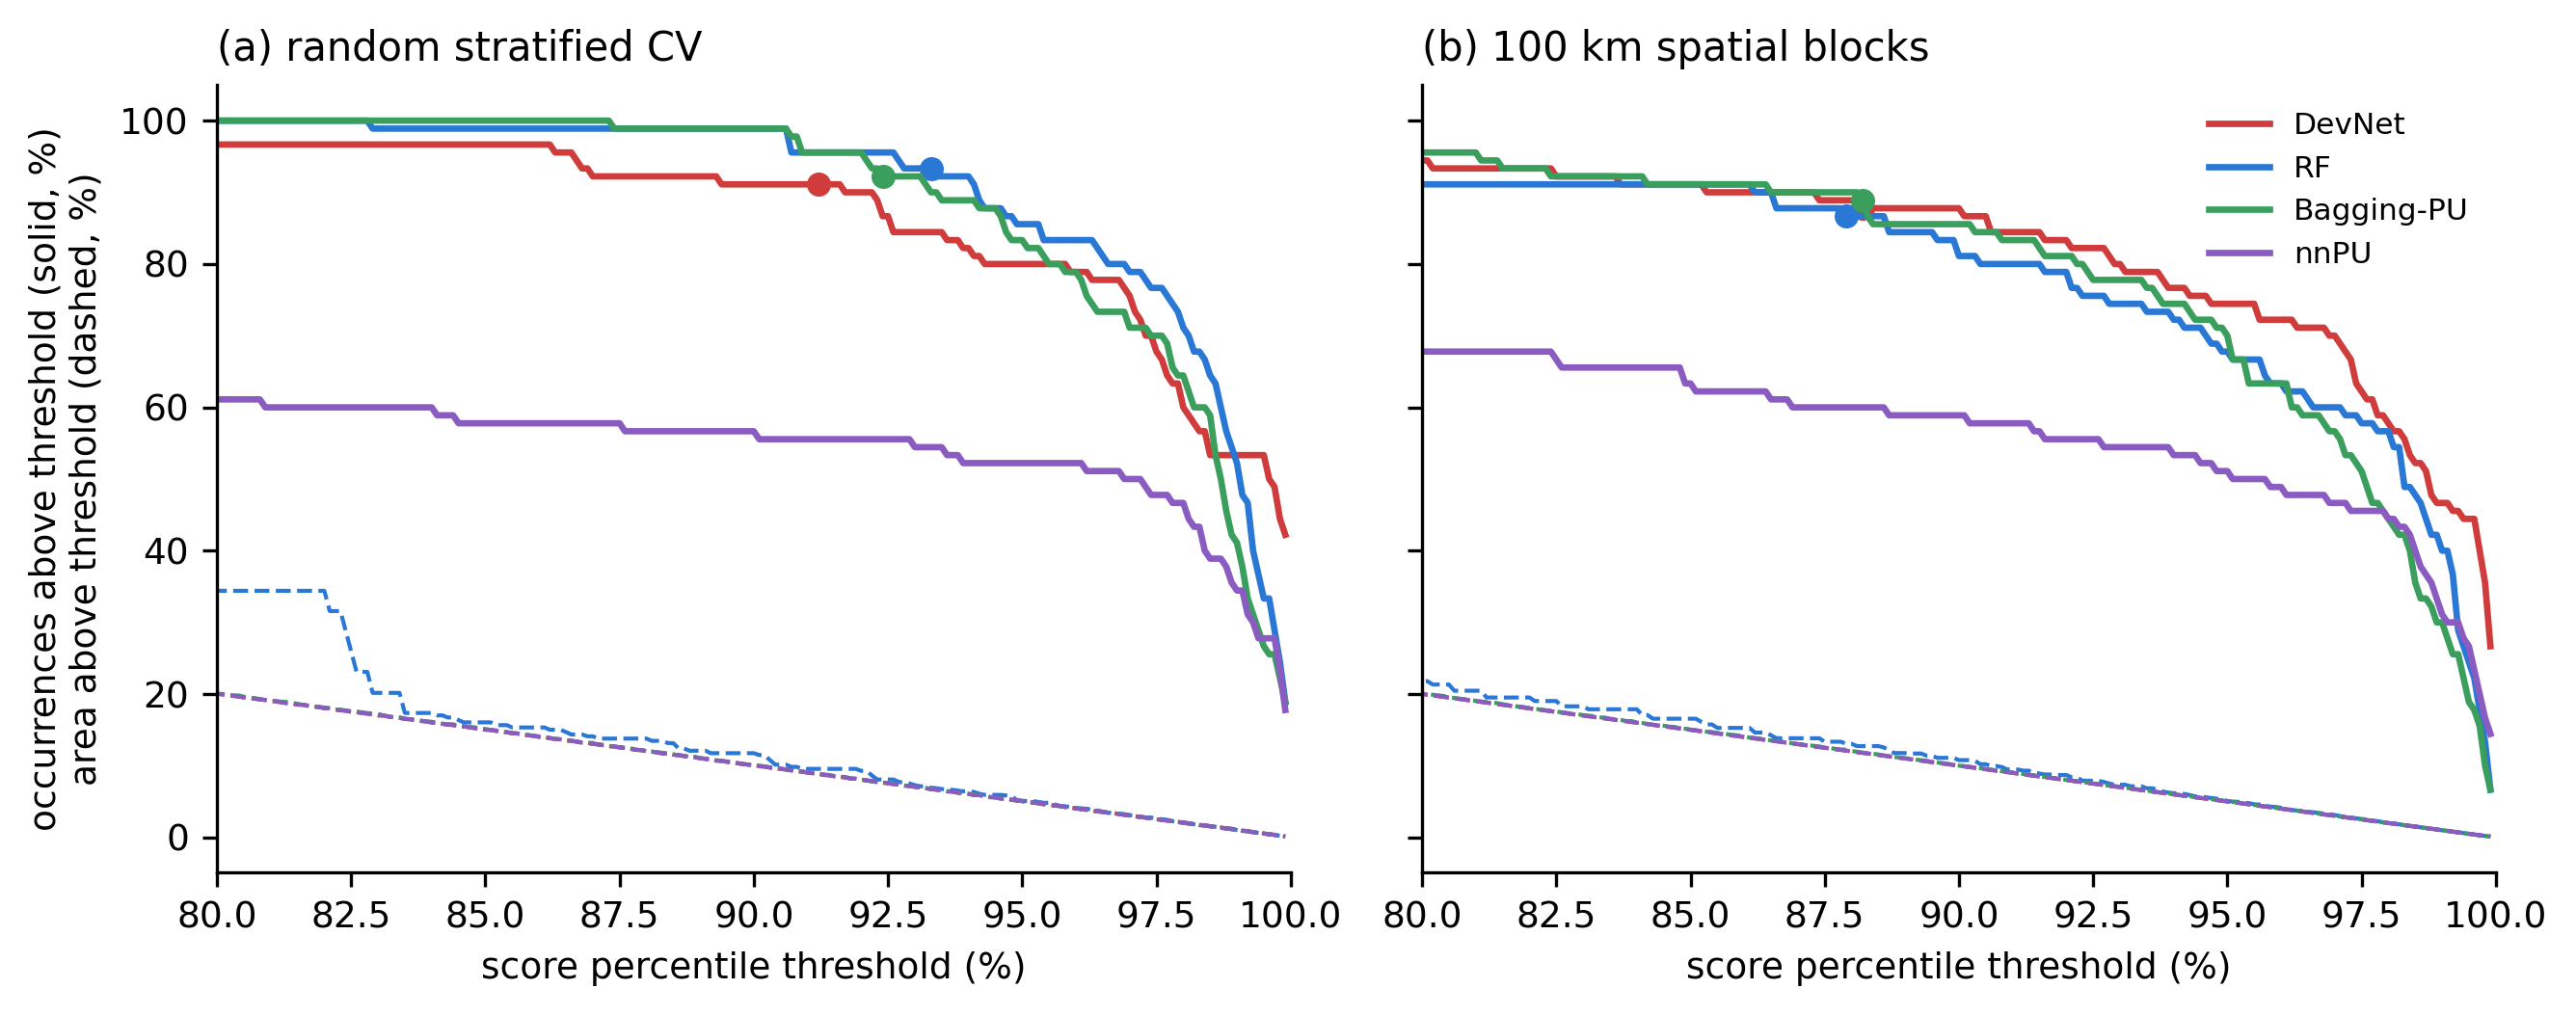
\includegraphics[width=0.9\textwidth]{figures/fig_pa_superior_r3.png}
\caption{Prediction--area curves for Superior from out-of-fold ranks: share of held-out occurrences (solid) and of the evaluation background, a proxy for area (dashed), above a score-percentile threshold; dots mark the intersections. (a) Random cross-validation, (b) 100~km spatial blocks.}\label{fig:pa}
\end{figure}

\begin{table}[!h]
\caption{Nested design selection: AP (median over six repeats) when DevNet's input transformation and batch composition are chosen inside each outer training fold by inner 100~km spatial cross-validation, compared with the final configuration and with RF. $\Delta$: paired difference on repeat-averaged ranks (repeats won). Chosen: outer folds choosing quantile 16+240 / quantile 16+16 / z-score 16+240 / z-score 16+16.}\label{tab:nested}
\scriptsize
\setlength{\tabcolsep}{2.5pt}
\begin{tabular*}{\textwidth}{@{\extracolsep\fill}llcccccc}
\toprule
Region & Split & Nested & Final & $\Delta$ vs final & RF & $\Delta$ vs RF & Chosen \\
\midrule
\multirow{4}{*}{Superior} & random & 0.354 & 0.445 & -0.055 & 0.271 & +0.155 (5/6) & 10/4/11/5 \\
 & 50 km & 0.335 & 0.418 & -0.046 & 0.192 & +0.194 (6/6) & 12/2/10/6 \\
 & 100 km & 0.312 & 0.343 & +0.023 & 0.168 & +0.219 (6/6) & 9/2/13/6 \\
 & 200 km & 0.190 & 0.252 & -0.064 & 0.151 & +0.120 (6/6) & 11/1/10/8 \\
\midrule
\multirow{4}{*}{Cordillera} & random & 0.335 & 0.341 & +0.010 & 0.427 & -0.083 (0/6) & 12/7/5/6 \\
 & 50 km & 0.133 & 0.129 & +0.057 & 0.092 & +0.068 (5/6) & 11/5/7/7 \\
 & 100 km & 0.069 & 0.055 & -0.004 & 0.046 & -0.034 (4/6) & 7/5/8/10 \\
 & 200 km & 0.062 & 0.076 & +0.000 & 0.039 & +0.000 (5/6) & 5/7/7/11 \\
\midrule
\multirow{4}{*}{Grenville} & random & 0.116 & 0.125 & +0.041 & 0.257 & -0.217 (0/6) & 16/10/1/3 \\
 & 50 km & 0.021 & 0.031 & -0.002 & 0.086 & -0.003 (0/6) & 20/6/1/3 \\
 & 100 km & 0.007 & 0.007 & -0.002 & 0.008 & -0.004 (2/6) & 16/6/2/6 \\
 & 200 km & 0.005 & 0.005 & -0.001 & 0.006 & -0.001 (0/6) & 17/5/1/6 \\
\botrule
\end{tabular*}
\end{table}

\begin{table}[!h]
\caption{Sensitivity of nnPU to the assumed class prior $\pi$, Superior (random cross-validation; median and 95\% interval over six repeats).}\label{tab:prior}
\footnotesize
\begin{tabular*}{0.6\textwidth}{@{\extracolsep\fill}lcc}
\toprule
$\pi$ & AUC & AP \\
\midrule
0.005 & 0.811 [0.779, 0.861] & 0.133 [0.099, 0.208] \\
0.01 & 0.838 [0.794, 0.892] & 0.152 [0.125, 0.191] \\
0.02 & 0.869 [0.825, 0.916] & 0.182 [0.143, 0.263] \\
0.05 & 0.902 [0.885, 0.924] & 0.264 [0.179, 0.311] \\
\botrule
\end{tabular*}
\end{table}

\clearpage
\section{Augmentation under spatially blocked validation}\label{app:aug-spatial}

\begin{table}[!h]
\caption{Superior average precision with fold-safe synthetic positives under spatially blocked cross-validation (median and 95\% interval over six repeats), with the paired per-repeat difference from no augmentation.}\label{tab:aug-spatial}
\footnotesize
\begin{tabular*}{\textwidth}{@{\extracolsep\fill}lllccc}
\toprule
Blocks & Model & Augmentation & AP & $\Delta$AP per repeat & wins \\
\midrule
100 km & DevNet & none & 0.343 [0.184, 0.452] & -- & -- \\
 &  & Gaussian jitter 10$\times$ & 0.336 [0.163, 0.456] & -0.000 [-0.024, +0.005] & 3/6 \\
 &  & SMOTE 3$\times$ & 0.346 [0.166, 0.448] & -0.006 [-0.020, +0.019] & 2/6 \\
 &  & WGAN-GP 3$\times$ & 0.342 [0.220, 0.541] & -0.005 [-0.063, +0.201] & 3/6 \\
 &  & WGAN-GP 10$\times$ & 0.321 [0.238, 0.395] & -0.031 [-0.095, +0.066] & 2/6 \\
\addlinespace
100 km & RF & none & 0.168 [0.067, 0.181] & -- & -- \\
 &  & Gaussian jitter 10$\times$ & 0.157 [0.070, 0.246] & +0.004 [-0.032, +0.072] & 5/6 \\
 &  & SMOTE 3$\times$ & 0.154 [0.059, 0.177] & -0.006 [-0.027, +0.005] & 1/6 \\
 &  & WGAN-GP 3$\times$ & 0.175 [0.093, 0.224] & +0.033 [-0.031, +0.051] & 5/6 \\
 &  & WGAN-GP 10$\times$ & 0.219 [0.091, 0.273] & +0.050 [+0.004, +0.101] & 6/6 \\
\addlinespace
200 km & DevNet & none & 0.252 [0.169, 0.342] & -- & -- \\
 &  & Gaussian jitter 10$\times$ & 0.247 [0.167, 0.336] & -0.005 [-0.009, +0.004] & 2/6 \\
 &  & SMOTE 3$\times$ & 0.246 [0.162, 0.365] & -0.003 [-0.014, +0.027] & 2/6 \\
 &  & WGAN-GP 3$\times$ & 0.260 [0.172, 0.334] & +0.001 [-0.027, +0.085] & 3/6 \\
 &  & WGAN-GP 10$\times$ & 0.248 [0.244, 0.317] & -0.006 [-0.035, +0.080] & 2/6 \\
\addlinespace
200 km & RF & none & 0.151 [0.106, 0.158] & -- & -- \\
 &  & Gaussian jitter 10$\times$ & 0.100 [0.076, 0.129] & -0.047 [-0.077, +0.014] & 2/6 \\
 &  & SMOTE 3$\times$ & 0.104 [0.055, 0.122] & -0.041 [-0.064, -0.005] & 0/6 \\
 &  & WGAN-GP 3$\times$ & 0.122 [0.089, 0.183] & -0.019 [-0.049, +0.042] & 2/6 \\
 &  & WGAN-GP 10$\times$ & 0.137 [0.093, 0.171] & -0.001 [-0.060, +0.049] & 3/6 \\
\botrule
\end{tabular*}
\end{table}

\clearpage
\section{Interpretation in the contrasting provinces}\label{app:shap}

\begin{table}[!h]
\caption{As Table~\ref{tab:shap}, Cordillera (55 features).}\label{tab:shap-cord}
\footnotesize
\begin{tabular*}{\textwidth}{@{\extracolsep\fill}lcccc}
\toprule
Feature & DevNet rank & DevNet dir. & RF rank & RF dir. \\
\midrule
Distance to regional high-grade metam. & 4 & $\downarrow$ (-0.97) & 1 & $\downarrow$ (-0.86) \\
Era: Mesozoic & 3 & $\downarrow$ (-0.82) & 14 & $\downarrow$ (-0.82) \\
Bouguer anomaly (BA) & 13 & $\downarrow$ (-0.96) & 3 & $\downarrow$ (-0.87) \\
Era: Proterozoic & 2 & $\uparrow$ (+0.67) & 18 & $\uparrow$ (+0.70) \\
Age contact (H3 cell) & 1 & $\uparrow$ (+0.85) & 34 & $\uparrow$ (+0.85) \\
Moho depth & 5 & $\uparrow$ (+0.96) & 10 & $\uparrow$ (+0.89) \\
Passive-margin proximity & 32 & $\uparrow$ (+0.73) & 2 & $\uparrow$ (+0.78) \\
Distance to regional age contact & 6 & $\uparrow$ (+0.96) & 11 & $\uparrow$ (+0.90) \\
DRTP mean (10 km) & 8 & $\downarrow$ (-0.95) & 7 & $\downarrow$ (-0.84) \\
Distance to regional greenstone & 30 & $\uparrow$ (+0.93) & 4 & $\uparrow$ (+0.20) \\
\botrule
\end{tabular*}
\end{table}

\begin{table}[!h]
\caption{As Table~\ref{tab:shap}, Grenville (58 features).}\label{tab:shap-gren}
\footnotesize
\begin{tabular*}{\textwidth}{@{\extracolsep\fill}lcccc}
\toprule
Feature & DevNet rank & DevNet dir. & RF rank & RF dir. \\
\midrule
Deep-source RTP & 1 & $\uparrow$ (+0.97) & 2 & $\uparrow$ (+0.73) \\
Distance to regional age contact & 4 & $\downarrow$ (-0.99) & 1 & $\downarrow$ (-0.77) \\
DRTP THD tilt & 9 & $\downarrow$ (-0.98) & 4 & $\downarrow$ (-0.80) \\
Distance to regional mafic-ultramafic & 15 & $\uparrow$ (+0.98) & 3 & $\uparrow$ (+0.45) \\
Distance to regional sedimentary & 11 & $\downarrow$ (-0.98) & 5 & $\downarrow$ (-0.91) \\
BA high-pass 40 km std. dev. (10 km) & 3 & $\uparrow$ (+0.98) & 8 & $\uparrow$ (+0.85) \\
DRTP mean (10 km) & 7 & $\uparrow$ (+0.97) & 14 & $\uparrow$ (+0.94) \\
Deep gravity-worm proximity & 2 & $\uparrow$ (+0.98) & 23 & $\uparrow$ (+0.80) \\
Deep magnetic-worm proximity & 6 & $\uparrow$ (+0.98) & 25 & $\uparrow$ (+0.80) \\
Moho depth & 20 & $\downarrow$ (-0.96) & 6 & $\downarrow$ (-0.68) \\
\botrule
\end{tabular*}
\end{table}

\clearpage
\section{Ablation of DevNet design choices}\label{app:sensitivity}

DevNet's two design choices (Section~\ref{sec:models}) are examined here with the inputs of the main analysis, by changing one element at a time from a configuration with z-scored inputs and label-balanced batches of 16 + 16 rows. All configurations are evaluated with the folds, protocols and seeds of the main results (Table~\ref{tab:ablation}). In Superior, quantile inputs alone raise AP under random splits from 0.358 to 0.424, and background-heavy batches alone to 0.395; together they give 0.445, the highest AP under every protocol except 100~km blocks, where the z-scored, background-heavy variant is level (0.349 against 0.343). Training for longer, by contrast, repeats the dozen positives and pushes the network towards memorising their neighbourhoods: with z-scored inputs, ten times more steps left random-split AP unchanged (0.361 against 0.358) but lowered it under 100~km blocks (0.277 against 0.329). The nested early-stopping configuration chooses the number of steps (100--3,000, cosine schedule over 3,000 steps) inside each outer training fold by a 100~km spatial cross-validation (three inner folds, two inner restarts, background purged from inner validation blocks), so the test fold is never used for the choice. Table~\ref{tab:margin} gives the sensitivity of the final configuration to the deviation margin: smaller margins gave somewhat higher AP in all three provinces (Superior 0.469 with $a = 2$ against 0.445 with $a = 5$), but we keep the value of \citet{Pang2019} rather than tune it on these folds.

\begin{table}[!h]
\caption{Ablation of DevNet's design choices: AP (median over six repeats) under random cross-validation and spatial blocks, on identical folds. Inputs: quantile-normal or z-scored; batch: positive\,+\,background rows per step; steps: number of gradient steps (nested ES: chosen by nested 100~km spatial cross-validation). In brackets: number of repeats in which the final configuration (bold) has the higher AP. --: not run.}\label{tab:ablation}
\scriptsize
\setlength{\tabcolsep}{2.5pt}
\begin{tabular*}{\textwidth}{@{\extracolsep\fill}llllllll}
\toprule
Region & Inputs & Batch & Steps & random & 50 km & 100 km & 200 km \\
\midrule
\multirow{6}{*}{Superior} & quantile & 16\,+\,240 & 300 (final) & \textbf{0.445} & \textbf{0.418} & \textbf{0.343} & \textbf{0.252} \\
 & z-score & 16\,+\,240 & 300 & 0.395 (4/6) & 0.380 (5/6) & 0.349 (3/6) & 0.221 (3/6) \\
 & quantile & 16\,+\,16 & 300 & 0.424 (5/6) & 0.347 (6/6) & 0.310 (5/6) & 0.239 (5/6) \\
 & z-score & 16\,+\,16 & 300 & 0.358 (6/6) & 0.332 (5/6) & 0.329 (4/6) & 0.226 (3/6) \\
 & z-score & 16\,+\,16 & 3,000 & 0.361 (6/6) & -- & 0.277 (4/6) & -- \\
 & z-score & 16\,+\,16 & nested ES & 0.367 (6/6) & 0.307 (5/6) & 0.262 (4/6) & 0.218 (6/6) \\
\midrule
\multirow{6}{*}{Cordillera} & quantile & 16\,+\,240 & 300 (final) & \textbf{0.341} & \textbf{0.129} & \textbf{0.055} & \textbf{0.076} \\
 & z-score & 16\,+\,240 & 300 & 0.297 (5/6) & 0.132 (4/6) & 0.078 (3/6) & 0.065 (4/6) \\
 & quantile & 16\,+\,16 & 300 & 0.301 (6/6) & 0.124 (6/6) & 0.047 (5/6) & 0.074 (2/6) \\
 & z-score & 16\,+\,16 & 300 & 0.271 (6/6) & 0.154 (4/6) & 0.085 (3/6) & 0.067 (4/6) \\
 & z-score & 16\,+\,16 & 3,000 & 0.228 (6/6) & -- & 0.060 (3/6) & -- \\
 & z-score & 16\,+\,16 & nested ES & 0.279 (6/6) & 0.128 (5/6) & 0.068 (4/6) & 0.057 (4/6) \\
\midrule
\multirow{6}{*}{Grenville} & quantile & 16\,+\,240 & 300 (final) & \textbf{0.125} & \textbf{0.031} & \textbf{0.007} & \textbf{0.005} \\
 & z-score & 16\,+\,240 & 300 & 0.072 (6/6) & 0.023 (5/6) & 0.005 (6/6) & 0.004 (6/6) \\
 & quantile & 16\,+\,16 & 300 & 0.122 (3/6) & 0.030 (5/6) & 0.006 (6/6) & 0.005 (6/6) \\
 & z-score & 16\,+\,16 & 300 & 0.059 (6/6) & 0.019 (6/6) & 0.006 (6/6) & 0.004 (6/6) \\
 & z-score & 16\,+\,16 & 3,000 & 0.105 (4/6) & -- & 0.005 (5/6) & -- \\
 & z-score & 16\,+\,16 & nested ES & 0.088 (4/6) & 0.028 (3/6) & 0.004 (6/6) & 0.004 (5/6) \\
\botrule
\end{tabular*}
\end{table}

\begin{table}[!h]
\caption{Sensitivity of DevNet to the deviation margin $a$ (AP, median over six repeats, random cross-validation). The main results use $a = 5$.}\label{tab:margin}
\footnotesize
\begin{tabular*}{0.7\textwidth}{@{\extracolsep\fill}lcccc}
\toprule
Region & $a = 2$ & $a = 3$ & $a = 5$ & $a = 8$ \\
\midrule
Superior & 0.469 & 0.453 & 0.445 & 0.436 \\
Cordillera & 0.367 & 0.369 & 0.341 & 0.313 \\
Grenville & 0.183 & 0.156 & 0.125 & 0.120 \\
\botrule
\end{tabular*}
\end{table}

\end{appendices}

\clearpage

\bibliography{references}

\end{document}
